\documentclass[12pt]{report}
\usepackage{amsmath}
\usepackage{graphicx}
\usepackage[top=5cm, bottom=3cm, left=2.5cm, right=2.5cm]{geometry} 
\usepackage{fancyhdr}
\usepackage{hyperref}
\usepackage{verbatim}
\usepackage{appendix}
\usepackage{subfig}
\usepackage[parfill]{parskip}
\graphicspath{{./docPics/}{./circuitDiagrams/}}

\pagestyle{fancy}
\lhead{\textbf{TELLIE Hardware Manual}}
\rhead{\textit{E. Leming, September 2016  (v1)}}

\newenvironment{itemize*}%
{\begin{itemize}%
\setlength{\itemsep}{0pt}%
\setlength{\parskip}{0pt}}%
{\end{itemize}}

\newenvironment{enumerate*}%
{\begin{enumerate}%
\setlength{\itemsep}{0pt}%
\setlength{\parskip}{0pt}}%
{\end{enumerate}}

\begin{document}
%%%%%%%%%%%%%%%%%%%%%%%%%%%%
% Title Page	
%%%%%%%%%%%%%%%%%%%%%%%%%%%%
\thispagestyle{empty}
\vskip40mm
\begin{center}
	% TITLE
	\LARGE\textbf{TELLIE hardware manual (v1)}
	\vskip5mm
	% SUBTITLE (optional)
	\large\textit{}
	%\vskip2mm
	% AUTHOR
	\large\textbf{E. J. Leming, R. White, J. Sinclair, S. Peeters, J. Waterfield, M. Stringer}
	\normalsize
	\vskip25mm
	\large\textbf{Latex source and figures at: \url{https://epp.phys.sussex.ac.uk/SnoPlus/Ellie}}
	\normalsize
\end{center}
%%%%%%%%%%%%%%%%%%%%%%%%%%%%
\tableofcontents
\newpage

%%%%%%%%%%%%%%%%%%%%%%%%%%%%%%%%%%%%%%%%%%%%%%%%%%%%%

\chapter{Introduction}
\label{sec:Intro}
This document is written for those interested in learning about the hardware associated with the TELLIE / AMELLIE optical calibration systems of SNO+. Although some details on how individual components are controlled and used are overviewed in this document, it does not provide a description of how to use the system as a whole. If that is your aim, please refer instead to the \textbf{TELLIE Users Manual}. At the time of writing this manual does not exist, as the DAQ code is under heavy development. When ready, it can be found at \cite{smellieHardwareMan}. In addition, this document will not provide the physics motivation for the inclusion of timing (TELLIE) and attenuation (AMELLIE) calibration sub-systems, nor does it describe any analysis of data generated by the systems. For a higher level overview of the system in the context of the experiment please see the JINST paper \cite{telliePaper}.

Before we get into the nitty gritty of all this, it is important to realise that, in every way but name (and LED wavelength), the TELLIE and AMELLIE subsystems are identical. In truth, they are two parts of the same system. They share identical LED driving and read out circuitry, are powered by the same power source, control signals are sent to both from the same \textit{control box} and they live in the same electronics rack. All hardware descriptions given in this document therefore refer to both TELLIE and AMELLIE. Considering this, for convenience, we'll henceforth use TELLIE to refer to both systems, unless explicitly stated otherwise.
 
An overview of the system architecture is given in this chapter, along with description of the two TELLIE operating modes. Chapters \ref{chap:PowerBox} through \ref{chap:inSitu} describe details of individual hardware components with the intention of being an exhaustive reference. For each component an introduction is given followed by a discussion of the component's specifications and functionality. Where appropriate, details have also been provided regarding the stand-alone operation of a specific component via computer control.

%%%%%%%%%%%%%%%%%%%%%%%%%%%%%%%%%%%%%%%%%%%%%%%%%%%%%

\section{Overview of TELLIE Hardware}

The TELLIE / AMELLIE systems (Timing / Attenuation Module of the Embedded LED / Laser Light Injection Entity) are just two of the subsystems of the larger ELLIE calibration system, which also includes a scattering module (SMELLIE). This, then, is the time to point out that SMELLIE is a laser array, completely different from the TELLIE / AMELLIE systems described by this document. If you wish to learn about SMELLIE, it has it's own Hardware manual \cite{smellieHardwareMan}.

TELLIE consists of hardware designed to generate short pulse width, fast rise time light, hardware to guide that light into the detector and software to control the light generation. The hardware can essentially be considered in terms of in-situ and ex-situ components. The in-situ components are those which are located in the SNO+ cavity. The ex-situ components are those which are based on the SNO+ electronics deck. The majority of the ex-situ hardware is the custom designed light production electronics. This includes an array of 96 LED driver boards capable of producing optical pulses with $\sim$ns widths, arranged into boxes of 8 channels per box. TELLIE has 96 channels (12 boxes). AMELLIE  has 8 channels (1 box). In total the system has 104 channels (13 boxes) of LED driver electronics. In addition to the LED driver electronics there is a custom power unit which distributes DC power to the system and a \textit{control box} which communicates with the individual driver channels and acts as the interface between TELLIE and it's control software. 

Once an LED has been fired, light travels from the LED to the detector via a chain of three PMMA optical fibres. First from the LED to a port on the output of LED driver box (0.75~m). Second from the driver box to a \textit{patch panel} (2~m) and finally from the patch panel to the SNO+ PMT Support Structure (PSUP) via a 45~m fibre length. A rough sketch of this configuration is shown in Figure~\ref{fig:SNO+_sketch}. In this arrangement the patch panel is used as the interface for connecting the in-situ components to the ex-situ ones. Additionally, in order to minimise the light leakage from the deck to the detector, a \textit{feed through box} was custom designed to properly handle passing the 45~m fibres into the detector cavity.

All control of the TELLIE system is handled through the aforementioned control box. This houses a Peripheral Interface Controller (PIC) chip, pre-compiled with a set of C functions which can be called with char commands, sent through a USB serial connection. A python class has been developed as a wrapper for sending commands to and receiving responses from the control box. During normal operation, an instance of this class is loaded into an xmlrpc server which runs on the DAQ1 machine. TELLIE is then operated via the ORCA DAQ system which acts as a client, calling class methods on the server. The server interprets these commands and sends on the relevant char commands to the TELLIE control box via a direct USB connection from the DAQ1 machine. 

One major advantage of this control design scheme is the python class can be used to control TELLIE from outside of ORCA. Simply connect a laptop directly into the control box's USB port and functions in the python wrapper class can be accessed via dedicated python scripts, allowing flexibility for bench top testing. 


\begin{figure}[htbp]
	\begin{center}
		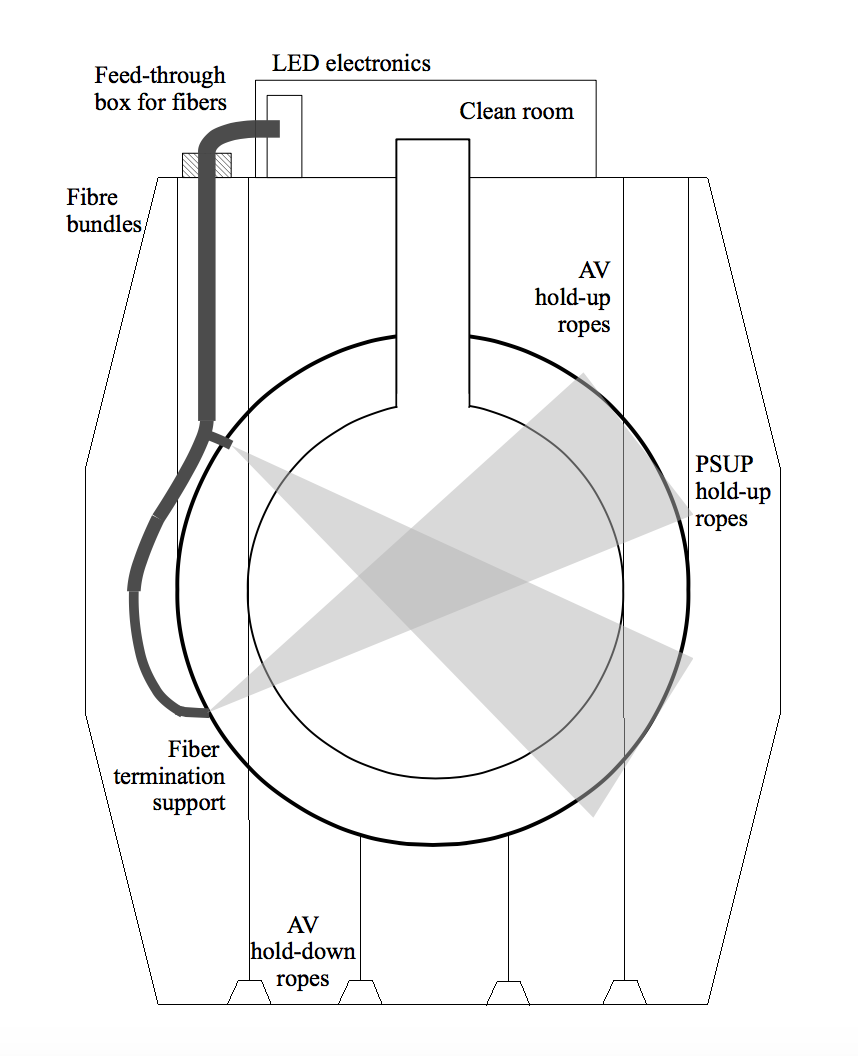
\includegraphics[scale=1]{TELLIE_in-situ}
		\caption{Sketch of the SNO+ detector showing the ELLIE calibration hardware. The ex-situ components can be seen on the deck, labelled LED electronics. The in-situ components (i.e. the 45~m optical fibres) can be seen reaching into the detector and attaching at example light injection positions on the PSUP.}
		\label{fig:SNO+_sketch}
	\end{center}
\end{figure}

\section{Operating Modes}
\label{subsec:OperatingModes}
TELLIE is designed to work in two possible modes: \textbf{master} and \textbf{slave}. The fundamental difference between these modes is the source of the signal that is used to trigger light generation. The choice of operating mode has an impact on the various timing delays that must be introduced into the detector readout chain to ensure that the all of the information associated with a single TELLIE event is collected and labelled as such within the SNO+ data structure.

A schematic of the optical and electronic timing contributions associated with the detector readout chain is given in Figure \ref{fig:ELLIE_timing}. In both operational modes the most important time is known as the \textbf{course delay}. This is the time between a TELLIE LED being triggered, and the Master Trigger Card Digital (MTCD) issuing a Global Trigger (GT) requesting the detector's PMT information be read out.\footnote{If terms like MTCD and GT are new to you it's recommended that you read the extensive trigger doc written by the Penn group during the electronics development for SNO \cite{snoTrigger}.}

\subsection{Timing considerations}

The timing schema associated with a SNO+ event is non-trival so before describing our specific electronics chain in detail, necessary for us to properly set the coarse delay, I will briefly summarise here. 

In normal physics running triggers are generated based on either the number of PMTs activated or the summed charge response of the hit PMTs. The logic chain used to identify such events is as follows. When an incident photon causes a charge pulse in a PMT it is checked against a discriminator threshold. If that threshold is crossed, a discrete \textit{trigger pulse} is generated for each SNO+ trigger types (NHit100, NHit20 etc.). Each electronics crate sums the \textit{trigger pulses} from each of it's associated channels and the sum is sent onto the analogue master trigger card (MTCA). In turn, the MTCA sums the signals from each crate and checks if any of the trigger types went above some global trigger threshold. If true, the MTCA will pass that information onto the MTCD. The MTCD then checks if the operator wants to acknowledge that trigger type by checking it against an allowed trigger mask. Finally, if that trigger type is ``masked in'' the MTCD will issue a GT back to the front end electronics on the rising edge of the next 50~MHz clock. 

The time for signals to travel through this chain (from the front end to the MTCD) is roughly 110 ns. Equally, the time for a GT to travel back from the MTCD to the front end, in doing so requesting the activated channels be read out, is also roughly 110 ns. This 220 ns total delay between the hit that caused the trigger sum to cross threshold (hit ‘x’) occurring at the front end, and the GT being received back at the front end defines the time between hit x occurring and the end of an event window. Hits are therefore recorded at the front end for 220~ns following hit x, and for (window\textunderscore size $-$ 220) ns preceding it. Historically the SNO(+) window size has always been set to 400~ns. All this is summarised in more details (with diagrams) in \cite{RATtime}.

What this means for TELLIE is that, if we want our light to appear in the middle of an event window, we require the MTCD to issue a GT $\sim$110~ns after the PMT signals reach the front end electronics. Exactly how a global trigger is requested depends on if TELLIE is operating in \textbf{master} or \textbf{slave} mode. 

Note: In reality 110~ns after the signals reach the front end is when \textit{physics} trigger requests will arrive at the MTCD (NHit 20, NHit 100 etc.). If more than one trigger arrives within a 20~ns window it's a random lottery as to which one will get tagged when the data gets built. For anyone analysing TELLIE data this is a problem as it will look like there are missing events in a TELLIE sequence. If we want TELLIE to consistently trigger off a hardware trigger the signal should arrive early to make sure it isn't hidden by a physics trigger. i.e. \textless110~ns after PMT signals reach the front end electronics, likely $\sim$90~ns.

\begin{figure}[htbp]
	\begin{center}
		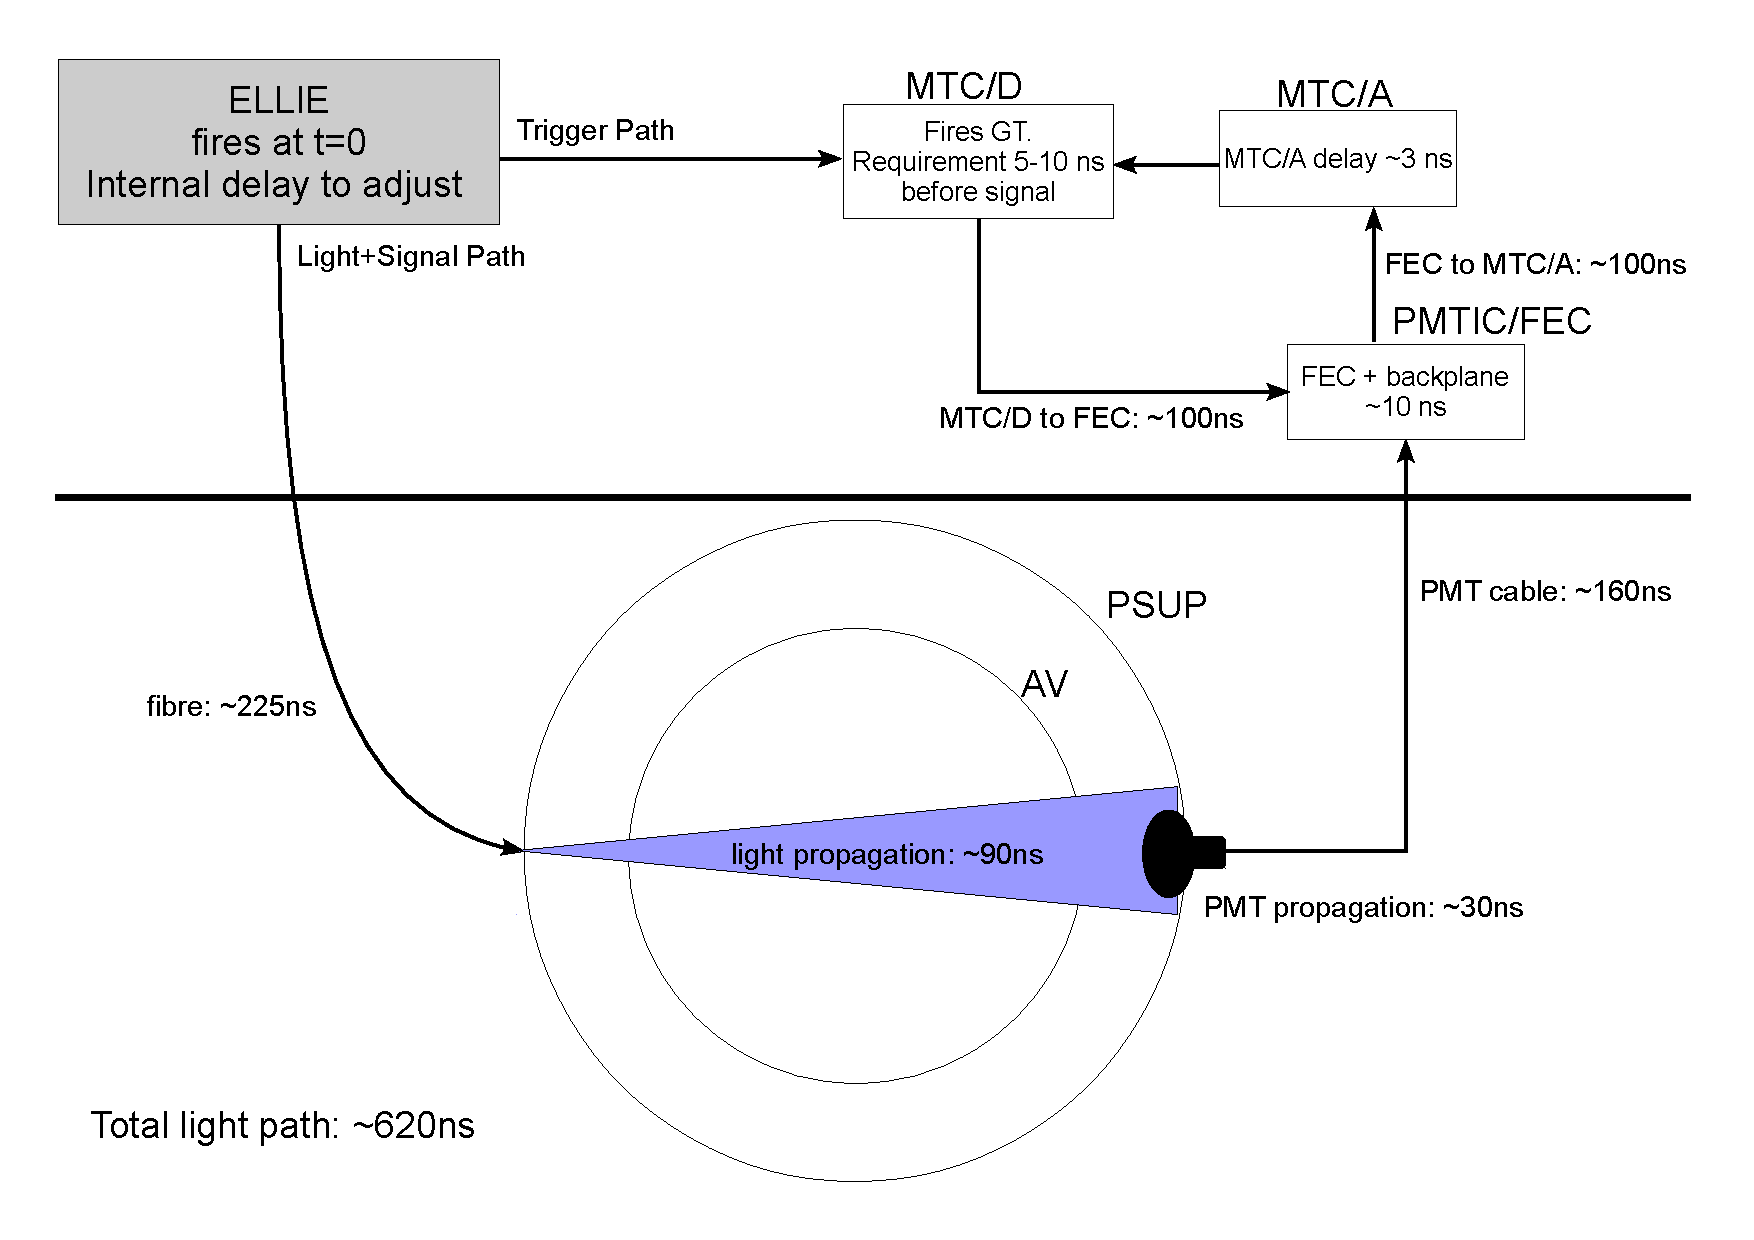
\includegraphics[scale=0.5]{ELLIE_timing}
		\caption{Schematic showing the time delay contributions from optical and electronic paths after the generation of a TELLIE light pulse.}
		\label{fig:ELLIE_timing}
	\end{center}
\end{figure}

\subsection{Master mode}

In master mode the primary signal (hardware selectable ECL/TTL type) is generated internally in the control box, the number and frequency of which are requested by the user. Receiving a primary signal causes two effects. 1) One or more TELLIE channels will generate an optical pulse 2) A trigger out signal is generated. %In actual fact, two trigger out signals are generated. One ECL type and one TLL type which are accessed via BNC feedthrough ports and the front and rear panel of the control box respectively, see section~\ref{sec:ControlBox}. 

The trigger out pulse is routed via a 20~m, 50~$\Omega$ coax cable to the trigger utility board, TUBii \cite{tubii}. TUBii was designed to handle and manipulate trigger signals for the whole detector system and adds a custom programmable delay to all of the ELLIE trigger out signals. The \textit{TUBii delay} for TELLIE must then be equal to approximately (620~ns - (20*0.7 / 3e8)) = \textbf{570~ns} (although in practice will require some tuning about this value to compensate for near AV reflections etc., which will could pre-maturely cause a physics trigger).

Once the delay has been applied, the delayed trigger line must be routed to the MTC/D's EXT-ASYNC trigger port via a short ($\sim$1~m) 50~$\Omega$ coax, terminated into a BNC. This port accepts trigger signals which are asynchronous to the MTC/D's internal 50~MHz clock. If another trigger port were to be used, where triggers are latched to the next rising edge of a clock cycle, an inherent 20~ns jitter would be introduced on an event to event basis. A jitter that large would make it impossible to calibrate the PMTs timing with TELLIE. 

A schematic showing the logic flow of associated with requesting and firing a sequence of 10 optical pulses in master mode is given in Figure~\ref{fig:TrigSchemaMaster}.

%By summing the various optical and electronic path delays shown in Figure~\ref{fig:ELLIE_timing}, we can calculate the total delay to be (225 + 90 + 30 + 160) = 505 ns. A trigger signal therefore needs to arrive at the MTCD 505 + 110 $\simeq$ 615~ns after the primary signal is received by TELLIE. 

\subsection{Slave mode}

The major difference in the schema associated with operating TELLIE in slave mode is that the primary signal is generated by TUBii, which has a dedicated trigger out channel for TELLIE. This is significant for two reasons. Firstly, TUBii is a custom designed trigger board and offers a more stable solution where all the parameters associated with the primary signal can be accurately tuned (Frequency, Pulse width, etc.). Secondly, TUBii generates and distributes the 50~MHz clock to the rest of the detector. Primary signals generated by TUBii are inherently latched to this clock. In theory, then, TELLIEs response can be perfectly synced with the detector system. This opens up the possibility of using a any of the standard trigger inputs on the MTC/D, not only the EXT-ASYNC. The only added timing jitter in this scenario is the jitter between the trigger in and trigger out signals. This is expected to be $\ll$1~ns. If any further timing jitter is observed in this modality it is recommended the trigger out is directed into the EXT-ASYNC. 

As described above, in slave mode the primary signal is generated by TUBii, which has a dedicated ECL trigger out channel for TELLIE. These ECL pulses are routed via a 20~m, 50~$\Omega$ coax cable from TUBii to the ECL trigger in port on the front of TELLIE's control box, see section \ref{chap:ControlBox}. The rate, pulse width and number of triggers in any sequence are variable parameters. Once the primary signal is received the resulting process is identical to that described in Master mode. Due to the control, flexibility and syncronisation with the wider detector system provided by the TUBii system, slave mode is the preferred operational mode. %That is, the trigger out ECL pulse from TELLIE is routed via a 20~m, 50~$\Omega$ coax cable back to TUBii. A delay (the \textit{TUBii delay}) is applied approximately equal to (615 - 20*0.7 / 3e8) = \textbf{570~ns}.

\begin{figure}[]
	\centering
	\subfloat[Master mode schematic]{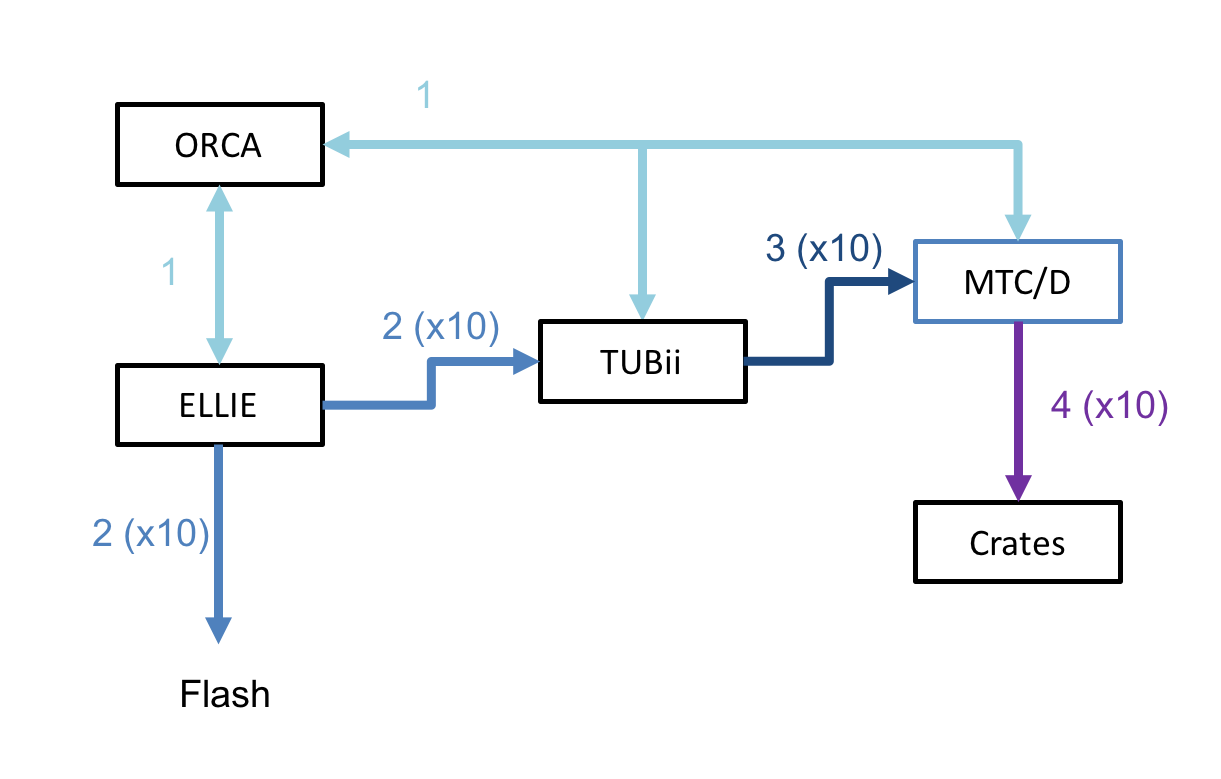
\includegraphics[width=0.8\textwidth]{TrigSchemaMaster} \label{fig:TrigSchemaMaster}}
	\newline
	\subfloat[Slave mode schematic]{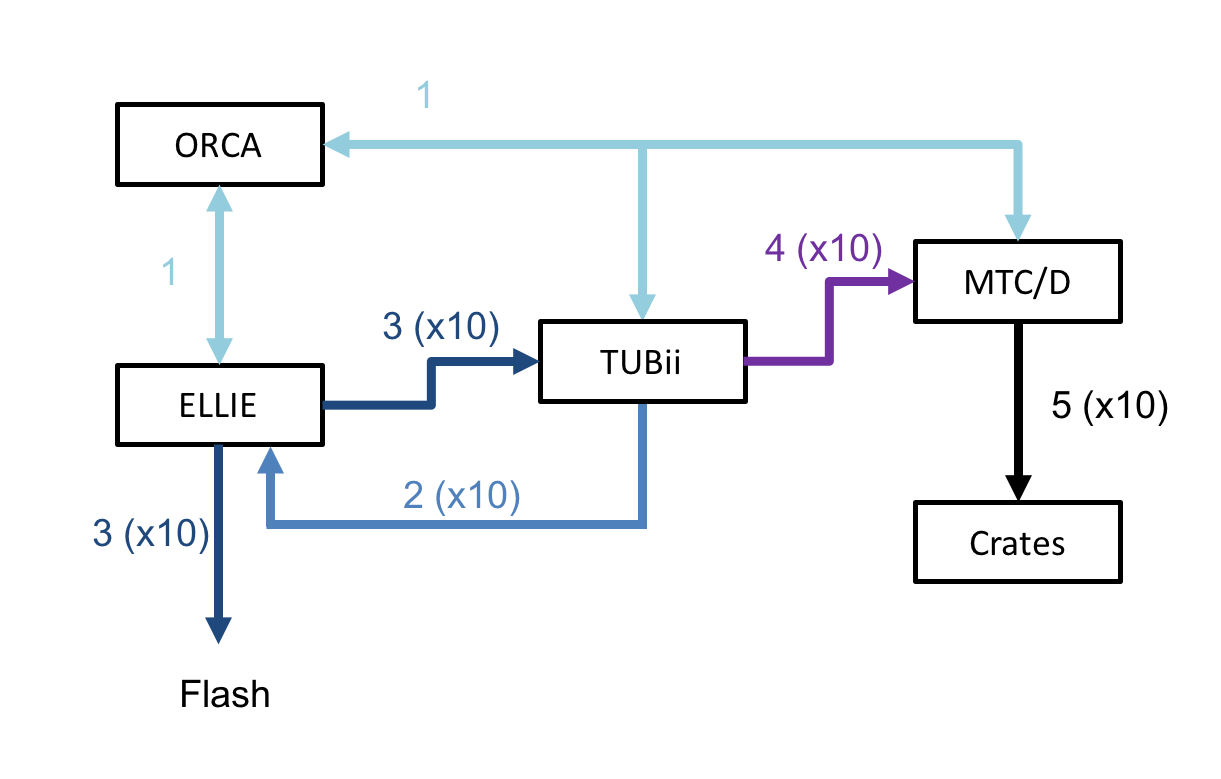
\includegraphics[width=0.8\textwidth]{TrigSchemaSlave} \label{fig:TrigSchemaSlave} }
	\caption{ELLIE triggering solutions. In both cases a sequence of 10 light pulses has been requested. Here the color coding and the numbers by the arrows refer to the ordering of the signals. The bracketed numbers (e.g. x10) refer to the number of signals sent via that line connection to produce a sequence of 10 flashes.}
\end{figure}

%\begin{figure}[htbp]

%%%%%%%%%%%%%%%%%%%%%%%%%%%%%%%%%%%%%%%%%%%%%%%%%%%%%

\chapter{Power box}
\label{chap:PowerBox}
The TELLIE system requires a set of specific DC voltages to operate its control box and all of its 95 LED driver \& PIN read out channels. TELLIE's power box distributes +5V, -5V and +7V DC power across the system via 8 pin DIN connectors and cables. For historical reasons a +9V line is additionally distributed down the cables, but is not accessed by the hardware. %The DIN connectors applied here were historically designed for analogue audio signals, but the numerous PINs allow for easy transit of a number of voltage lines with extremely robust mechanical connections.  

Three DC voltage supplies are used: +5V, -5V and +9V, with the +7V line being produced via a small voltage divider circuit on the +9V line. Originally all three supplies were switch mode type. These are more efficient than linear mode versions and produce much less heat, but after observing some fluctuations on the +5V line the switch mode type supply was replaced with a beefier linear mode version. After this upgrade fluctuations were still observed, which were eventually tracked to poor connections in the built in fuse housings. The offending fuse housings were bypassed by using automobile type fuses (from Canadian tyre :)), which attach directly onto the power cables. The power cables connected into the new fuses can be observed in the bottom left hand corner of Figure~\ref{fig:PowerBoxInside}. 

Since the described modifications were completed at SNOlab (Summer 2015) no fluctuations in the Power Box's output have been observed. However, due some unexplained instabilities in the LED driver \& PIN readout response a mains filter has been added between the TPS box used to supply the ELLIE electronics rack (tps-ellie1.sp.snolab.ca) and the mains input seen on Figure~\ref{fig:PowerBoxAnnotations} as a precaution. 


\section{Physical interface}

The physical interface for TELLIE's power box is extremely simple. It includes a mains power connection, a power switch, a number of historic fuse housings (now defunkt) and 14 DC power output connectors (each an 8 pin DIN type). Photographs of both the front and rear faces of the box are shown in Figure~\ref{fig:PowerBoxAnnotations}.

The DIN connectors have a two stage fastening system. First the pins should be properly aligned and pushed into an available socket. Second there is a screw fastening which must be pushed forward and tightened to the thread on the outside of the socket. The screw stage should always be properly completed to be certain there are no loose connections in the system.   

\begin{figure}
	\centering
	\subfloat[]{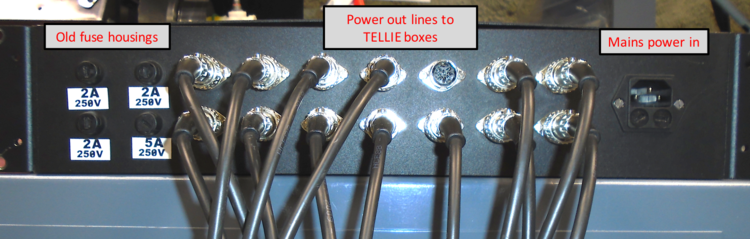
\includegraphics[width=1.0\textwidth]{PowerBoxFront}} 
	\newline
	\subfloat[]{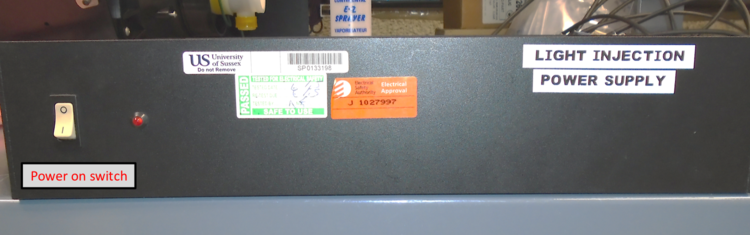
\includegraphics[width=1.0\textwidth]{PowerBoxBack}}
	\caption{Photographs of TELLIE's power box, annotated with points of interest (a) Front face (b) Rear face.}
	\label{fig:PowerBoxAnnotations} 
\end{figure}


\section{Board designs \& description}
The schematic design of TELLIE's power box is given in Figure~\ref{fig:PowerBoxSchematic}, a photograph showing inside the box itself is given in Figure~\ref{fig:PowerBoxInside}. The design is extremely straight forward and simply links the voltages to colour-coded lines, which are distributed to the relevant connector pins from the `probe points' shown in Figure~\ref{fig:PowerBoxInside}.

\begin{figure}[htbp]
	\begin{center}
		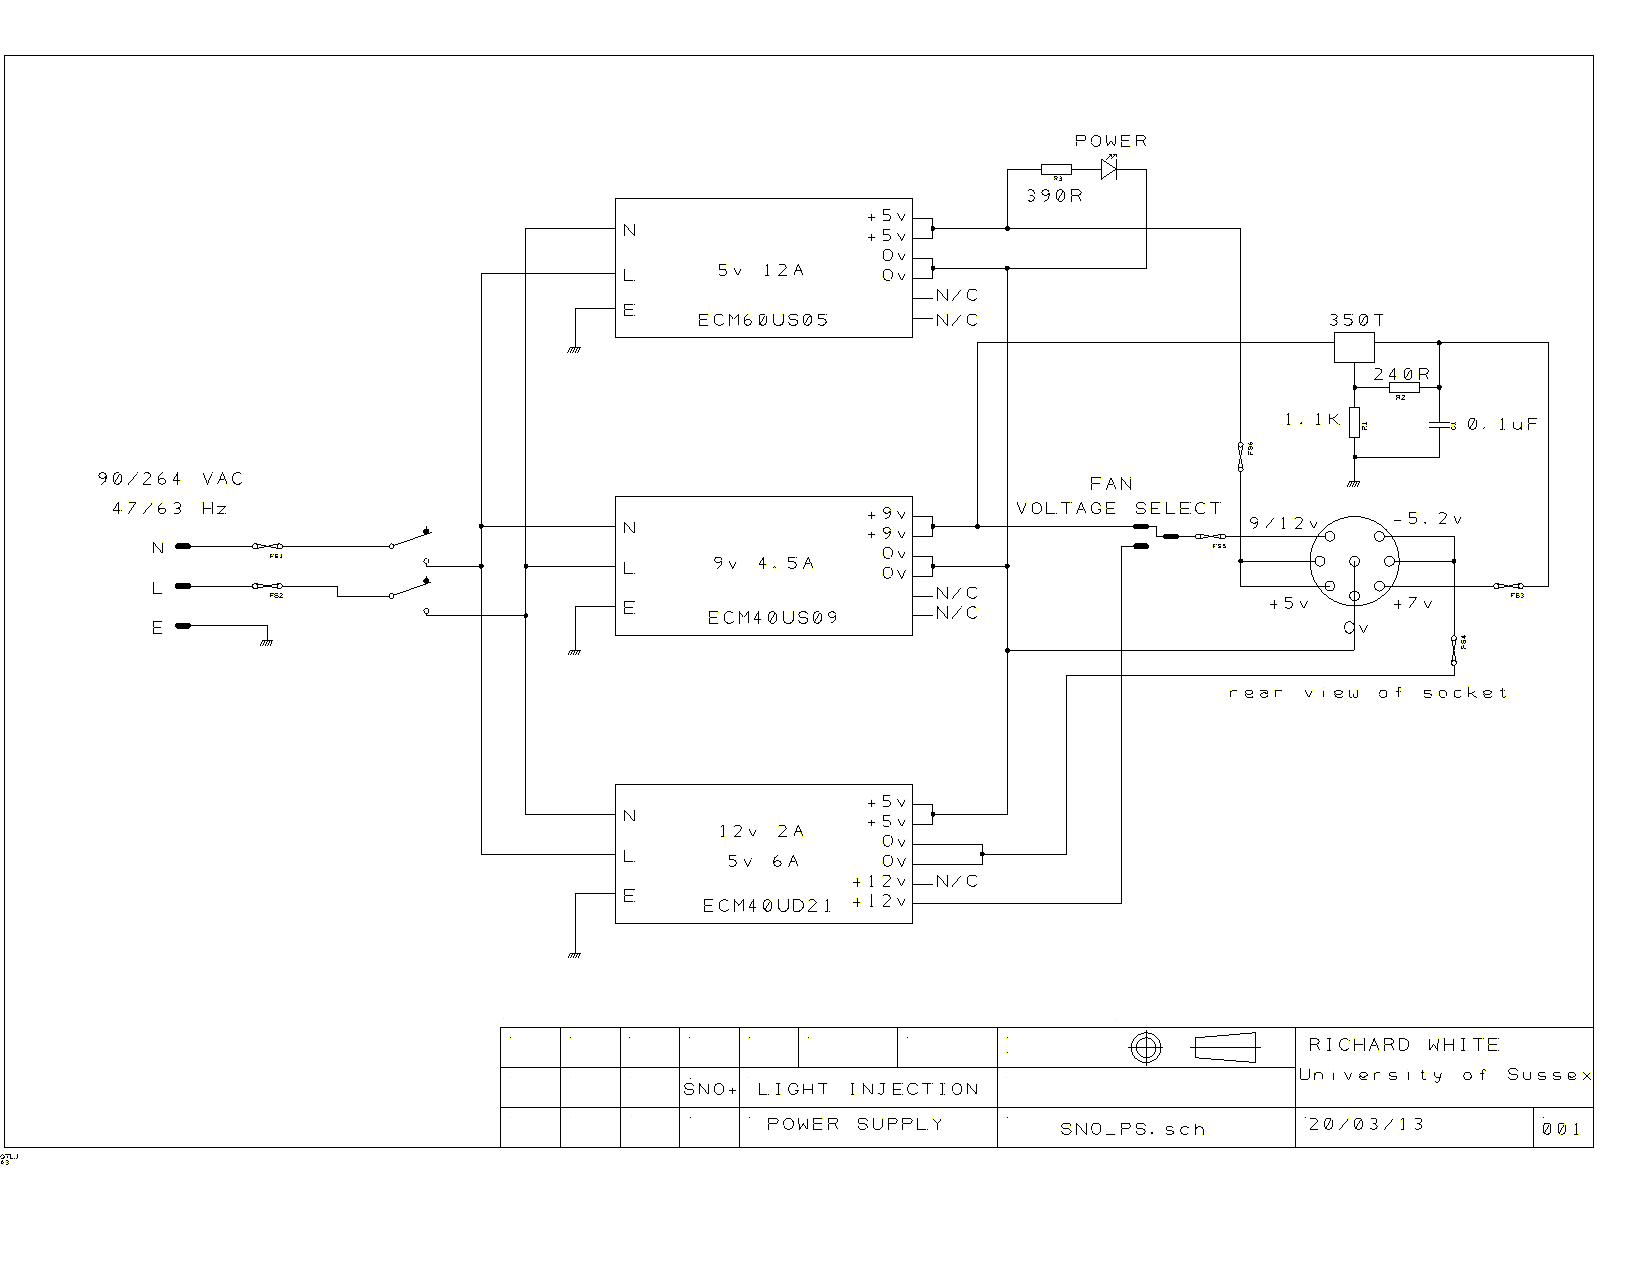
\includegraphics[width=1.0\textwidth]{PowerBoxSchematic}
		\caption{Schematic design of the TELLIE power box, including the voltages supplied to the DIN connector pins.}
		\label{fig:PowerBoxSchematic}
	\end{center}
\end{figure}


\begin{figure}[htbp]
	\begin{center}
		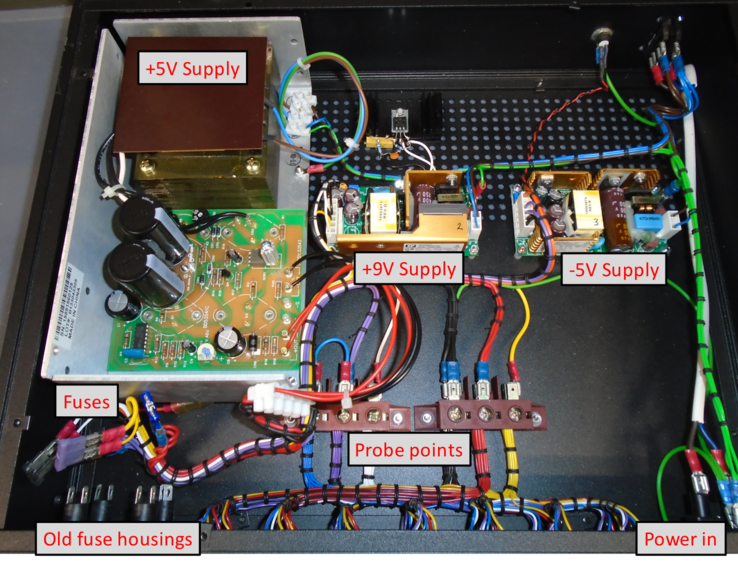
\includegraphics[width=1.0\textwidth]{PowerBoxInside}
		\caption{Photograph inside the TELLIE power box.}
		\label{fig:PowerBoxInside}
	\end{center}
\end{figure}

\section{Remote power cycling}
Although not strictly a function of TELLIE's power box, it is possible to remotely power cycle the TELLIE system via the networked power switch (NPS-8H20-ATS-1), often referred to as a TPS, which supplies AC mains power to the power box. To do so, one must first be on the SNO+ VPN \cite{NetworkManual}. Once connected to the VPN server one can simply ssh into the TPS at the address: super@tps-ellie1.sp.snolab.ca. A password is required which is subject to change, the current password is available on request from SNO+ network group: snoplusnetwork@googlegroups.com. On successful creation of an ssh portal, a splash screen will appear with instructions for how to turn the power on / off to the available ports, which are named. The port that TELLIE is plugged into has been re-named `TELLIE'. The TELLIE system can then be power cycled by following the provided commands.

\textbf{Please note:} cutting the power via the TPS is equivalent to simply pulling the plug out of the wall. It should only be done with very good reason! If a power cycle is absolutely necessary, it is always preferable to do so manually, using the power switch shown in Figure~\ref{fig:PowerBoxAnnotations}b. 

\chapter{Control box}
\label{chap:ControlBox}
All interactions TELLIE has with the wider detector / DAQ systems happen through the control box. Essentially it exists as an interface, accepting and interpreting analogue and digital inputs and, in turn, generating relevant outputs. Before discussing the hardware in detail, this introductory section will be used  to give a description of the logic flow associated with signals passing through the control box and how these go on to form an optical event. 

The first step in requesting and optical signal from one (or more) tellie channels is to request some electronics parameters be set which will define: which driver board is to be addressed, the frequency, the intensity and the number of resulting signals. To do so, digital commands can be communicated through serial communication ports, after which they are interpreted by a local PIC chip. The chip has been pre-compiled with a set of C functions, each of which can be called with a single char command. Any commands piped to the chip are stored in an internal buffer and processed in serial. The chip responds by interpreting the commands (and any associated variables), applying the requested settings and priming the system to accept primary signals (or triggers). If the system has been set to accept externally generated signals, the analogue ``trigger\textunderscore in'' input is additionally activated \footnote{In reality two trigger\textunderscore in ports exist, one ECL and one TTL, on the front and back of the control box respectively. It is only possible to active one of these at any given instant, the selection for which is made on the hardware. This is discussed in detail in section \ref{subsec:controlBoardDesign}.}. 

At this stage there are three distinct reactive states which TELLIE may have been put in: fire continuous, fire single or fire sequence. Fire continuous is the most simplistic case. Here TELLIE will continuously accept primary signals, generating an optical pulse and trigger out on receipt of each. The PIN diode response will be ignored. Fire single is slightly more complex in that it also handles the PIN diode response. A single primary signal will be accepted, a single optical pulse and trigger out pulse pair produced, and a single PIN reading returned to the PIC chip. The PIC then displays the returned value on an internal buffer, which can be queried via the serial communication ports. Finally, the fire sequence state builds on the basic functionality of fire single. In this case the number of primary signals of interest must be set by the user (16 bit integer 0-65535). The PIC chip then uses an internal counter to count through the specified number of primary signals, produces an optical and trigger out pulse pair for each and reads back the PIN diodes response. During this process a function in the chip keeps a running total of the sum and sum$^2$ of all the PIN readings returned in this sequence. At the end of a sequence the chip uses these values to calculate the mean and rms PIN response, which is returned to the internal buffer for querying.  Once the counter has reached the requested limit (i.e. the sequence has completed) the trigger ports are de-activated, meaning any further trigger signal received will be ignored.

This basic operational logic allows a user to: request a customisable optical pulse from each of the 96 channels, produce optical pulses at a frequency defined either by an internal oscillator or by an external trigger source and monitor TELLIE's response in the form of a trigger out signal and an independent measurement of the optical pulse amplitude in the form of a PIN diode measurement. 

\section{Physical interface}
\label{sec:ControlBoxInterface}
This section describes the features of the control box's physical interface and should be used as a reference when ``plumbing in'' any I/O connections. Photographs overviewing the physical interface are presented in Figure \ref{fig:ControlBoxAnnotations}. 

\subsection{Digital ports}
The control box has a total of four separate digital I/O ports: one B-type USB port and three RS232 serial connections. For general operation only the USB port is of interest, providing a direct link to the DAQ1 machine underground which hosts the TELLIE server. The two are connected by a 20~m eithernet cable terminated at a ethernet-to-USB converter which couples into the USB communication port shown in Figure~\ref{fig:ControlBoxAnnotations}a. An eithernet cable is used due to the DAQ1 machine having a large eithernet port hub (additionally, eithernet is generally considered the better option for communicating over distances greater than 5~m).

Each of the three RS232 ports was designed with an individual purpose.

%\begin{itemize}
	The port on the front left of the box, shown in Figure~\ref{fig:ControlBoxAnnotations}a, is an alternative to the USB port for serial communication with the PIC chip. By default this port is not active. To activate, a TELLIE expert is required to remove the USB connection on the board itself, which can be seen just below jumper 3 in Figure~\ref{fig:ControlBoard}, replace it with the equivalent connector from the RS232 port and mount a max 232 chip into the empty holder just to the right. The chip acts as an extra layer of interpretation required for the RS232 standard. As a result this port is entirely mutually exclusive with the USB port, only one can be active at any one time.

	The port on the front right of the box is a historical artefact. It is completely disconnected and has no purpose. Please ignore.

	The port on the back of the box was included as a selected data output line. It was originally intended for a live display showing the current settings as stored on the PIC chip. The functionality was never finalised. Please ignore.
	
%\end{itemize}

\subsection{Analogue ports}
The control box has a number of analogue ports, as can be seen in Figure~\ref{fig:ControlBoxAnnotations}. These can be separated into three fundamental types: power transmission, trigger ports and communication to LED driver boxes. 

%\begin{itemize}
	The power\textunderscore in port is an 8 pin female DIN connector and receives +5V, -5V, +7V and +9V DC, from TELLIE's power box. More information on these connectors is given in Chapter~\ref{chap:PowerBox}.

	The trigger ports are all 50~$\Omega$ BNC type and are split between the front and back face of the box. The ECL trigger\textunderscore in and trigger\textunderscore out ports are on the front face and the equivalent TTL ports on the back face. Both port pairs are labelled on the hardware to identify the input and output appropriately. Note: These two trigger port pairs are totally mutually exclusive i.e. only one set can be active at any one time! The selection is made by a set on jumpers on the PCB within the box, described section~\ref{subsec:controlBoardDesign}. 

	Finally there are two 37 pin ribbon connector ports in the centre of the box's front face, see Figure~\ref{fig:ControlBoxAnnotations}a. The ports send and receive signals to and from the LED driver boxes. Communications to boxes 1-6 and boxes 7-12 are sent via the lower and upper connectors respectively.  
%\end{itemize}


\subsection{Indicators}

Finally, there are two LEDs on the control box's front face: one red and one green. The red LED illuminates when the box is properly powered. The green LED flashes when TELLIE receives a primary signal, and is often used as a debugging tool. At rates of approximately 100~Hz or greater it will appear that the green light is on continuously. 


\begin{figure}
	\centering
	\subfloat[]{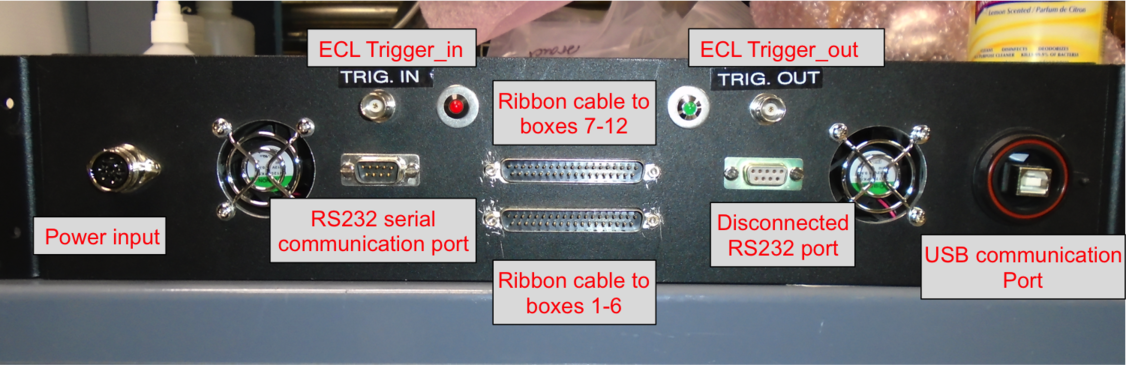
\includegraphics[width=1.0\textwidth]{ControlBoxFront}} 
	\newline
	\subfloat[]{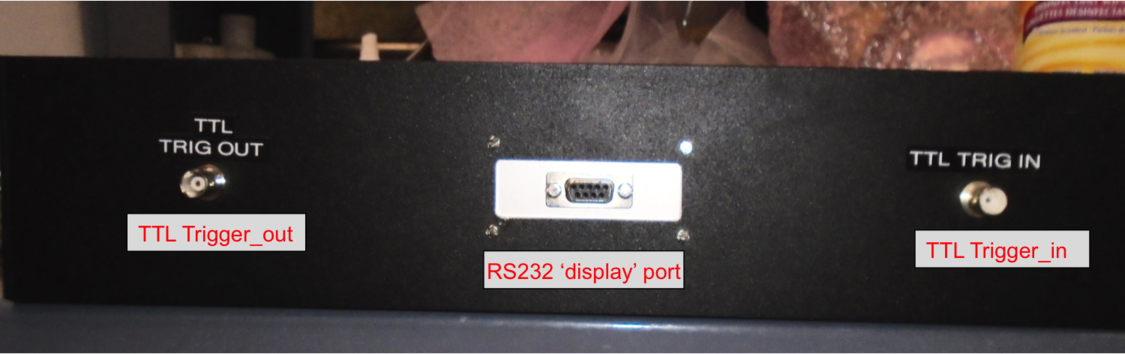
\includegraphics[width=1.0\textwidth]{ControlBoxBack}}
	\caption{Photographs of TELLIE's control box, annotated with points of interest (a) Front face (b) Rear face.}
	\label{fig:ControlBoxAnnotations} 
\end{figure}

%All LED driver settings and triggering logic are handled by the control box's internal PIC chip, which also interprets the 14 bit digital signal returned by the PIN diode readout boards in response to an optical pulse.  

\section{Board designs \& description}
\label{subsec:controlBoardDesign}
The control board PCB was custom designed by Richard White at the University of Sussex, a description of which is shown in Figure~\ref{fig:ControlBoardDesign}. The design centres around a PIC chip which can generate both analogue and digital controls pulses which are bussed to the LED driver boxes via a ribbon cable connection. 

There are a number of hardware tunable variables on the control board itself, each are varied with a custom jumper. The positions of these jumpers have been identified on both the board design and board photograph given in Figures~\ref{fig:ControlBoardDesign} and \ref{fig:ControlBoard} respectively. The purpose of these jumpers is as follows:

\begin{enumerate}
	\item Connects the bias to a ECL-to-TTL converter circuit. This jumper is on the boards for historical reasons. In an earlier design the ECL / TTL trigger types did not have physically separate BNC ports. This converter circuit had to be connected in and out depending what type of trigger was to be supplied. Since the final design includes physically separate lines for the different trigger signals it is no longer an issue, \textbf{this connector should never be removed}.
	\item As described earlier in this document, the ECL / TTL trigger I/O port pairs are mutually exclusive. This jumper defines which of the two trigger port pairs are active. \textbf{Note: these jumpers are labelled incorrectly on the board! The TTL position will activate the ECL ports and vice versa}. 
	\item Selects the polarity of the trigger\textunderscore in. Polarity settings are as labelled on the board. 
	\item These define a course timing delay on the trigger\textunderscore out signal. The single jumper shown in Figure~\ref{fig:ControlBoardDesign} is split into two sets of jumpers on the board in Figure~\ref{fig:ControlBoard}: a bottom set with three positions and a top set with two. The time delays associated with these jumper positions are as follows: bottom set from left to right, 100, 60, 20~ns. Top set from left to right 80, 40~ns. Figure~\ref{fig:ControlBoard} shows a blue jumper in the middle position of the bottom set, resulting in a 60 ns delay.
	\item Polarity of the tigger\textunderscore out signal. Polarities settings are as labelled on the board.
\end{enumerate}

\begin{figure}[htbp]
	\begin{center}
		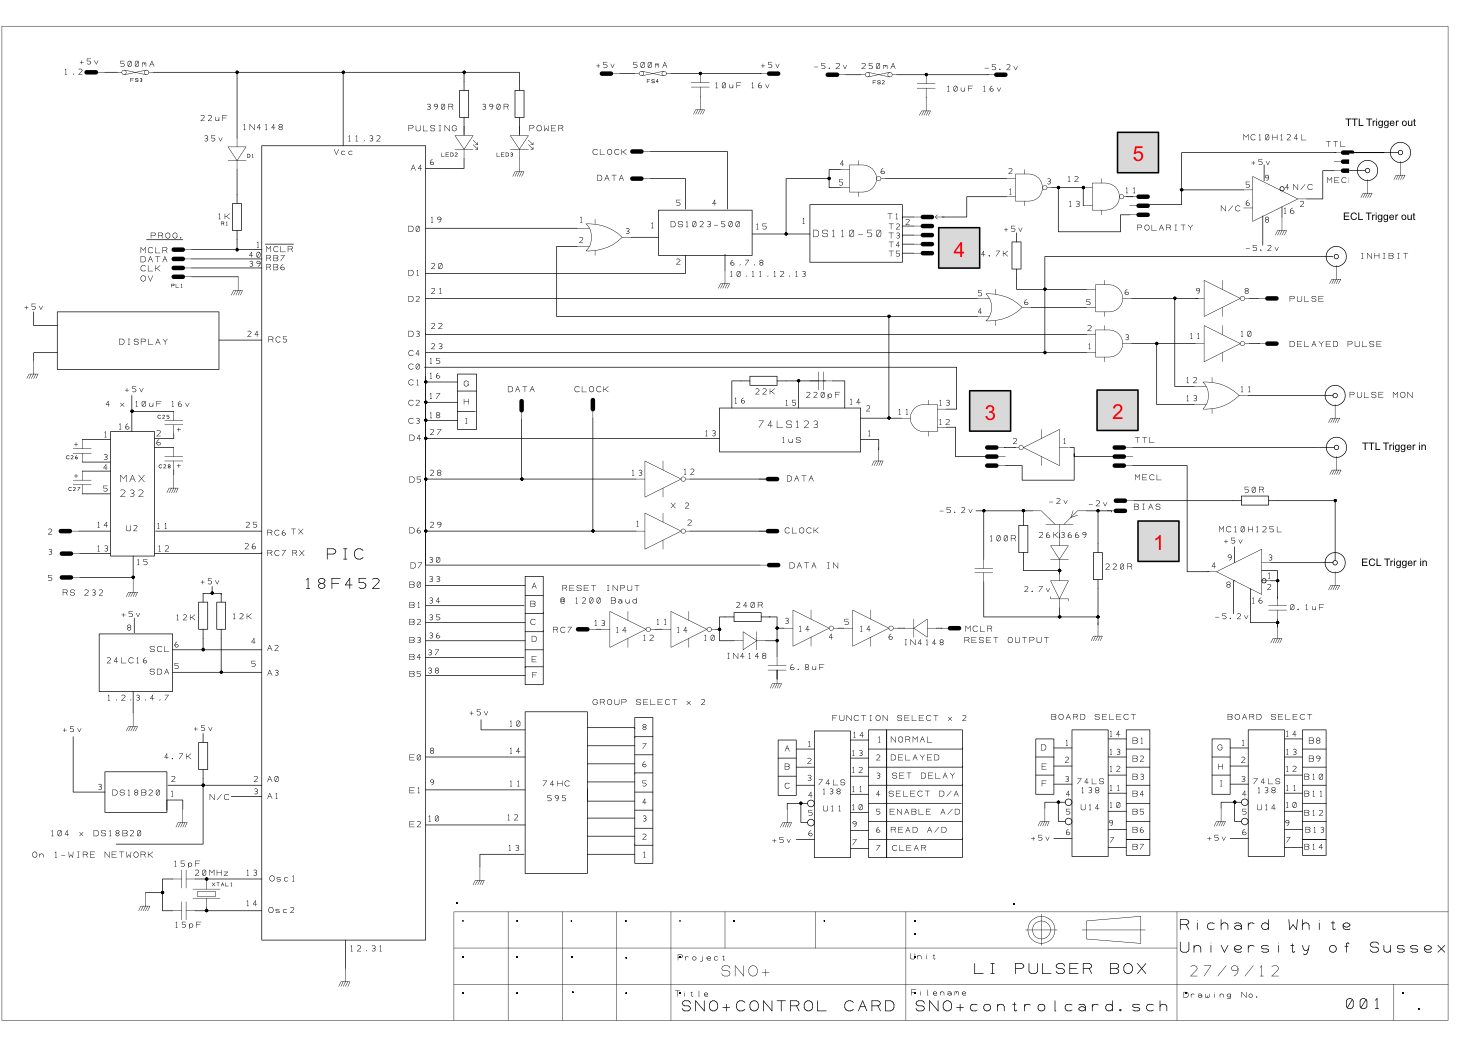
\includegraphics[width=1.0\textwidth]{ControlBoardPCB}
		\caption{Technical design of TELLE's control board. Jumpers included in the board's design have been labelled 1-5.}
		\label{fig:ControlBoardDesign}
	\end{center}
\end{figure}

\begin{figure}[htbp]
	\begin{center}
		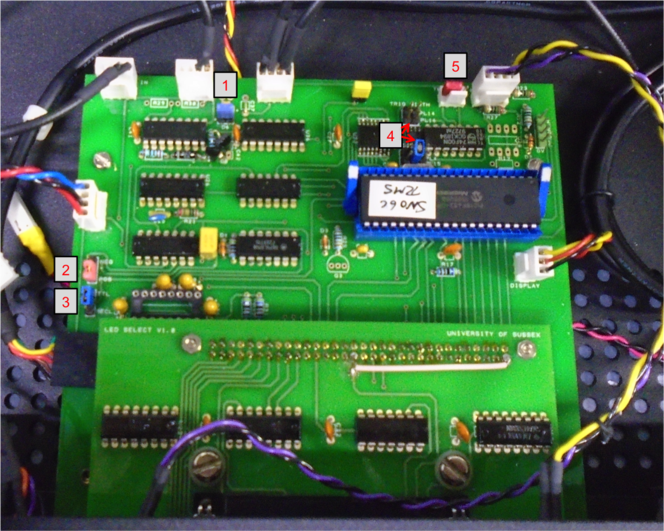
\includegraphics[width=1.0\textwidth]{ControlBoardInside}
		\caption{Photograph inside the TELLIE control box showning the PCB layout. Jumpers included in the board's design have been labelled 1-5.}
		\label{fig:ControlBoard}
	\end{center}
\end{figure}


\section{Controllable parameters}
This brief section describes the parameters required to control TELLIE's response to a primary signal. These can be split into two basic types. Control of trigger O/I and control of LED drivers and optical pulses. 

The trigger I/O control parameters are: \textit{Number of pulses}, \textit{Trigger delay} and in the case of master mode operation only, \textit{delay between pulses}. All three of these parameters are global controls, meaning they are applied identically regardless of which LED driver channel is being addressed. Historically the trigger delay parameter was designed to provide the delay necessary to centre the generated optical pulse in the SNO+ event window. This job has since been delegated to TUBii. The TELLIE trigger delay should therefore be set to 0 as a default. The number of pulses variable primes the system to receive primary signals. In slave mode a counter is used to count the number of externally generated trigger signals received by the box. Once the requested number has been reached the trigger in ports are de-activated and any subsequent signals will be ignored. In master mode the number of pulses variable is used to define how many primary signals are internally generated. Finally, in the case of master mode, delay between pulses is also required to define the temporal separation between subsequent generated signals. It should be noted that master mode triggers are software generated (C code on the PIC chip). This has two major effects: The generation of pulses at a requested frequency is not very accurate (although the jitter has been measured to be low), and the max rate hits a limit at around $\sim$10kHz.

The LED drivers are complex systems and require a number of parameters to properly define a requested optical pulse. First is \textit{channel selection}. This can either be done with a single integer or, if the user would like to request multiple channels be activated, with an array of integers. In each case only integers between 1-112 represent valid addresses of TELLIE LED driver channels. With a channel selected the parameters which define the current pulse to be pushed through the LED must be set. The available parameters are the \textit{current pulse height} ($I_{OP}$) and textit{current pulse width} ($I_{PW}$), both are described in detail in Section~\ref{sec:LEDdrivers}. It was observed during early characterisation tests at Sussex that varying the $I_{OP}$ would give inconsistent and unpredictable results when comparing across driver boards. As a result this values is always set to its maximum, 16383 (14 bit integer).The $I_{PW}$ value is therefore the only parameter that should be varied to influence the light generation of the selected channel(s). The $I_{PW}$ has a 14 bit dynamic range (0 - 16383) where the intensity of the optical signal is inversely proportional to the set value, i.e. $I_{PW}$ = 0 gives the maximum possible optical signal and $I_{PW}$ = 16383 the minimum possible. In reality all boards stop producing light once $I_{PW}$ \textgreater$\sim$ 7000. Finally, a \textit{fibre delay} can be applied to the LED driver trigger signals. This is a \textbf{channel dependent delay}, applied by a variable delay line built onto each diver board. Its purpose is to compensate for board-to-board variations in the time between a primary signal being received at the control box and light being produced at the requested channel. These variations are due in part to cable delays, but also the response of individual driver chips and LEDs. 

Due to the limited register size in the PIC chip itself, plus the dynamic range of both driver and delay chips, the parameters used to set the above described parameters have limited ranges. Table~\ref{tab:parrange} below summarises all parameters available to control TELLIE's response. Included are the valid integer inputs for each variable, how the PIC chip interprets these inputs, and the resulting output.  

A suite of python classes and scripts has been written to handle the serial communication to and from the TELLIE control box \cite{tellieCode}. This suit handles the relevant type conversions to allow a user to set the three delays in terms of the units given in the final column of Table~\ref{tab:parrange}.

%\textbf{Note on the frequency.} The frequency is set by the pulse delay parameter. The range given in the table~\ref{tab:parrange} is the maximum that the hardware allows, but for operating the equipment more safely it has been reduced. Instead of (approximately) 4~Hz to inf., it is brought down to 4~Hz to 10~kHz. When the board is operated in slave mode, the external trigger bypasses the pulser chip, and the maximum frequency was set to 10~kHz as well.

\begin{table}%[]
	\begin{center}
		\begin{tabular}{|c|c|c|c|c|c|}
			\hline
			Parameter Name & Settable Range & Internal Hi/Lo  & PIC & Resulting Dynamic  \\
			& & Bit Splitting & Interpretation & Range\\
			\hline
			Channel & 0 - 255 & Hi 0 - 255 & Hi & 0 - 255 \\
			& valid: 1 - 112 & & & valid: 1 - 112  \\
			\hline
			Pulse Width & 0 - 16383 & Hi 0 - 63 & (Hi*256)+Lo & 0 - 16383 \\
			& & Lo 0 - 255 & & \\
			\hline
			Pulse Height & 0 - 16383  & Hi 0 - 63 & (Hi*256)+Lo & 0 - 16383\\
			& & Lo 0 - 255 & & \\
			\hline
			Fibre Delay & 0 - 255 & Hi 0 - 255 & Hi*0.25 & 0 - 63.75 [ns] \\
			(Channel dependent) & & & & step: 0.25  \\
			\hline
			\hline
			Trigger Delay & 0 - 255 & Hi 0 - 255 & Hi*5 & 0 - 1275 [ns] \\
			(Global) & & & & step: 5  \\
			\hline
			Number of Pulses & 0 - 65535 & Hi 0 - 255 & Hi*Lo & 0 - 65025\\
			& & Lo 0 - 255 & & step: variable \\
			\hline
			Delay Between & 0 - 65535 & Hi 0 - 255 & Hi+(Lo*4) & 0.004 - 256 [ms] \\
			Pulses & & Lo 0 - 255 & [ms] [$\mu$s] & step: variable\\
			(Master Mode) & & & & \\
			\hline
		\end{tabular}
	\end{center}
	\caption{List of the TELLIE control parameters. The table shows the accepted input range for each field (ranges are defined by 8, 14 or 16 bit integer types), how those integers are interpreted by the PIC chip and the resulting dynamic range for each parameter. Where appropriate units have been given to the calculated output values.} 
	\label{tab:parrange}
\end{table}

\section{PIC chip}
\label{sec:PICChip}
The PIC chip is the heart of the control box. As already described it receives and interprets ASCII commands sent via serial communication with the box. The chip is programmed in C, the code for which can be found at \cite{PIC code}. Being a limited memory device, a specific compiler must be used to generate a compatible executable. Generally, C18 is the go-to compiler of choice. ASK DICK. What compiler? What hardware used to house chip during memory write? What software used for memory write?

\chapter{TELLIE driver box}
\label{chap:DriverBox}
The bulk of the real estate in the TELLIE hardware rack is populated with twelve LED driver boxes. Each box contains eight \textit{channels}, where a channel is defined by a driver coupled to an LED, which itself couples directly into a 0.75~m optical fibre. The fibre terminates at an ST connector on the box's outer casing. The drivers are mounted on a motherboard that is connected to the control box. Each LED is contained within a brass ``cone'', a PIN diode is mounted at the opposite end of the cone, monitoring the LED's output at each pulse. The eight PIN diodes are mounted on two PIN boards, four left and four right, see Figure~\ref{fig:DriverBoxSchematic}.

The driver boxes are connected to the control box via a ribbon cable, onto which up to seven can be daisy-chained. As the control box has ports for two ribbon cables, upto fourteen driver boxes can be connected. However, TELLIE only uses twelve boxes and AMELLIE one, leaving one spare connection. On each driver box motherboard there are a set of jumpers next to the control box connection, which identifies the driver box to the control box, as box 1 to 7. Driver box 1 contains channels 1 to 8, box 2 channels 9 to 16 and so on, until channel 112 in box 14. To address a specific channel, only its number is needed.

Each PIN diode has two potentiometers, that allow the PIN's gain and sample point to be set. Ideally the gain would be set to allow maximal sensitivity to the low light levels without saturating at higher levels. However, the majority of TELLIE's work will be done at low light outputs ($\sim$1e3 photons), and with a limited dynamic range, the gain has been set to optimise the sensitivity in this region. Typically the PIN response will saturate above $\sim$5e5 photons / pulse, although the actual value will vary channel-to-channel. 


\begin{figure}[htbp]
	\begin{center}
		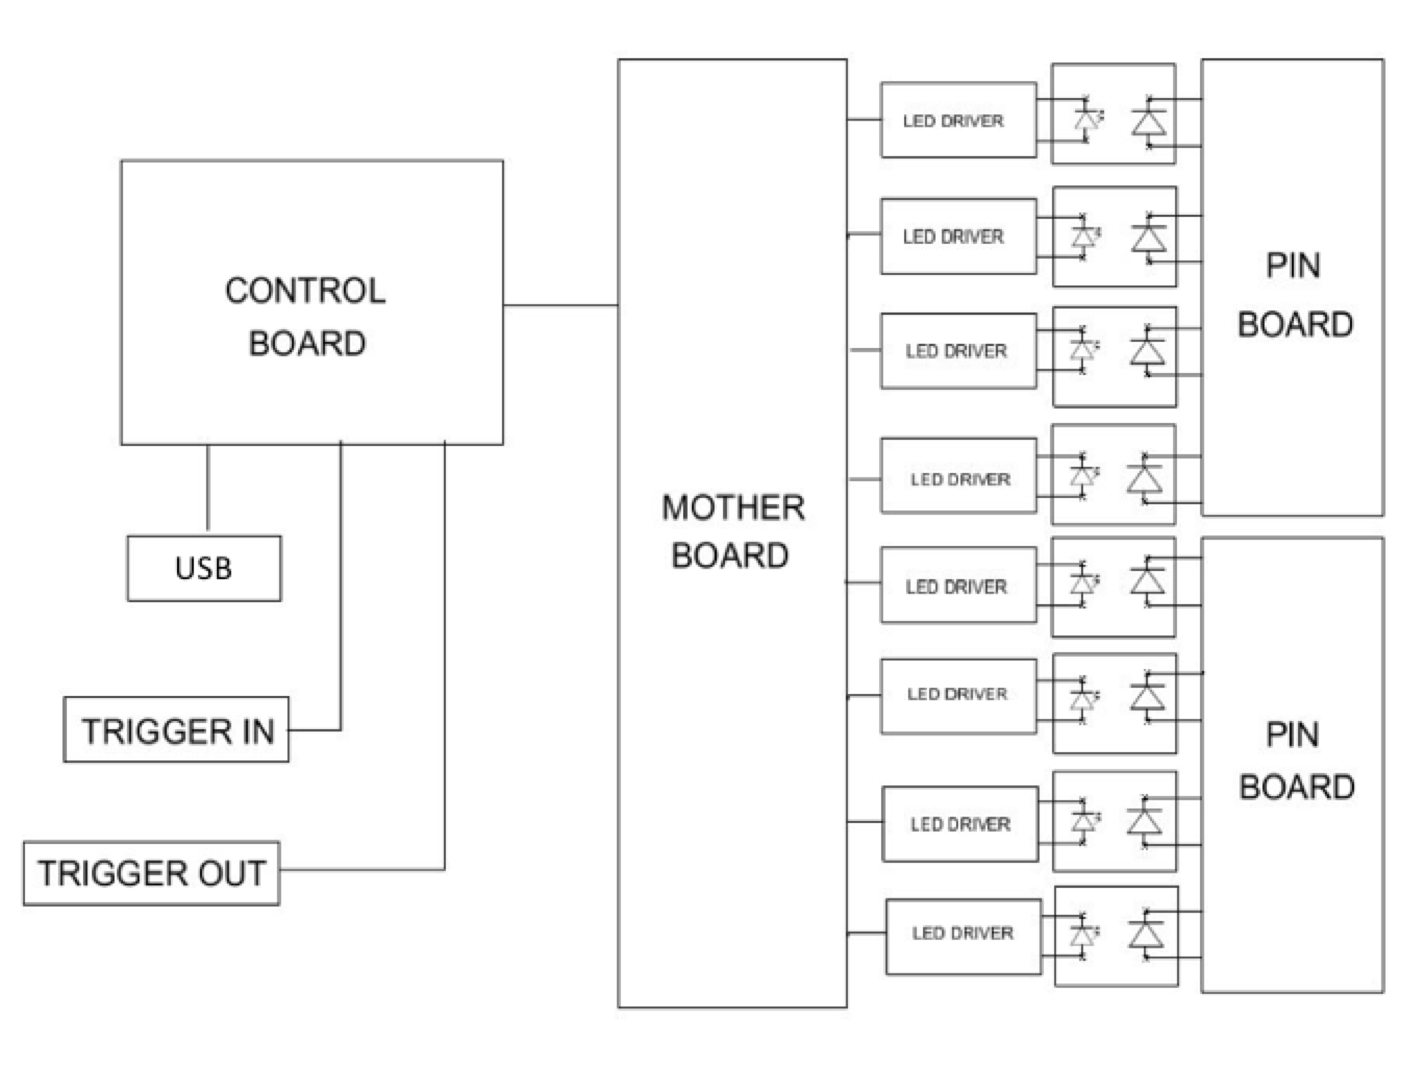
\includegraphics[width=0.6\textwidth]{DriverBoxSchematic}
		\caption{A schematic of the TELLIE driver box showing the basic connections to the control box and the position of the PIN diode boards monitoring LED output.}
		\label{fig:DriverBoxSchematic}
	\end{center}
\end{figure}

\section{Physical Interface}
\label{sec:DriverInterface}
The physical interface of a driver box, shown in Figure~\ref{fig:DriverBoxAnnotated}, is relatively straight forward. The driver channels output through ST connectors on the front face which are numbered from left to right in increasing order. When in place in the TELLIE rack on deck 2~m patch fibres are used to couple light from these output connectors to the ELLIE patch pannel. 

Aside from the eight optical connectors there are three electrical connections on the front face of box: Two power input connections, one on either side of the front face, and a 37 pin connector in the centre to host the ribbon cable from the control box. Despite having two power inputs, only one should ever be populated. Two were included in the design to allow for flexibility when routing cables from TELLIE's power box, both are completely equivalent and either can be used at any time. 

As is described in the caption for Figure~\ref{fig:DriverBoxAnnotated}, it should be noted that the order of the channels and their outputs is reversed relative to each other. This is a design feature included to minimise the bend required to couple the 0.75~m optical fibres to their associated ST connector.

\begin{figure}[htbp]
	\begin{center}
		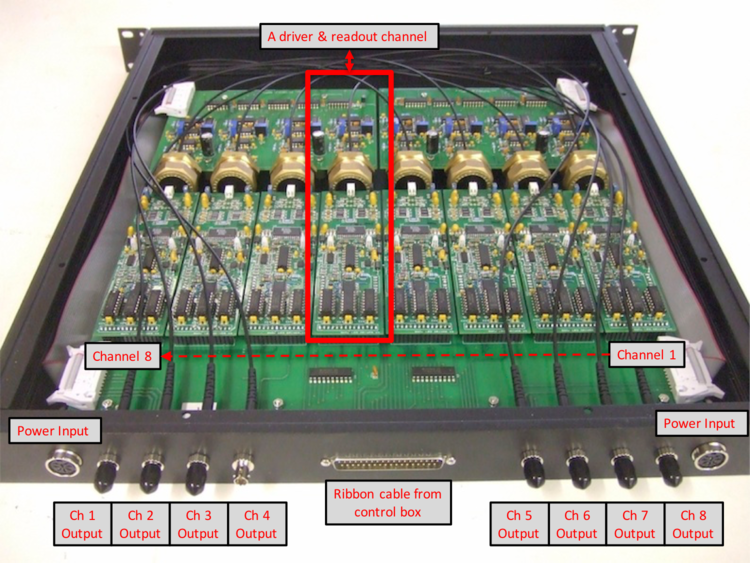
\includegraphics[width=0.7\textwidth]{DriverBoxAnnotated}
		\caption{A photograph showing one of TELLIE's LED driver boxes. Note: The ordering of the channels and their outputs are reversed relative to each other. This is to minimise the bending of the internal 0.75~m optical fibres. Other annotations are further discussed in the text.}
		\label{fig:DriverBoxAnnotated}
	\end{center}
\end{figure}

The ribbon cable data connection into each box transfers all the information to and from the control box. If some issue occurs in the communication chain it may be necessary to debug in individual data lines. The descriptions of the pins and jumpers present on a control box mother board are shown in Figure~\ref{fig:LEDBoxMotherboard}. 

\begin{figure}[htbp]
	\begin{center}
		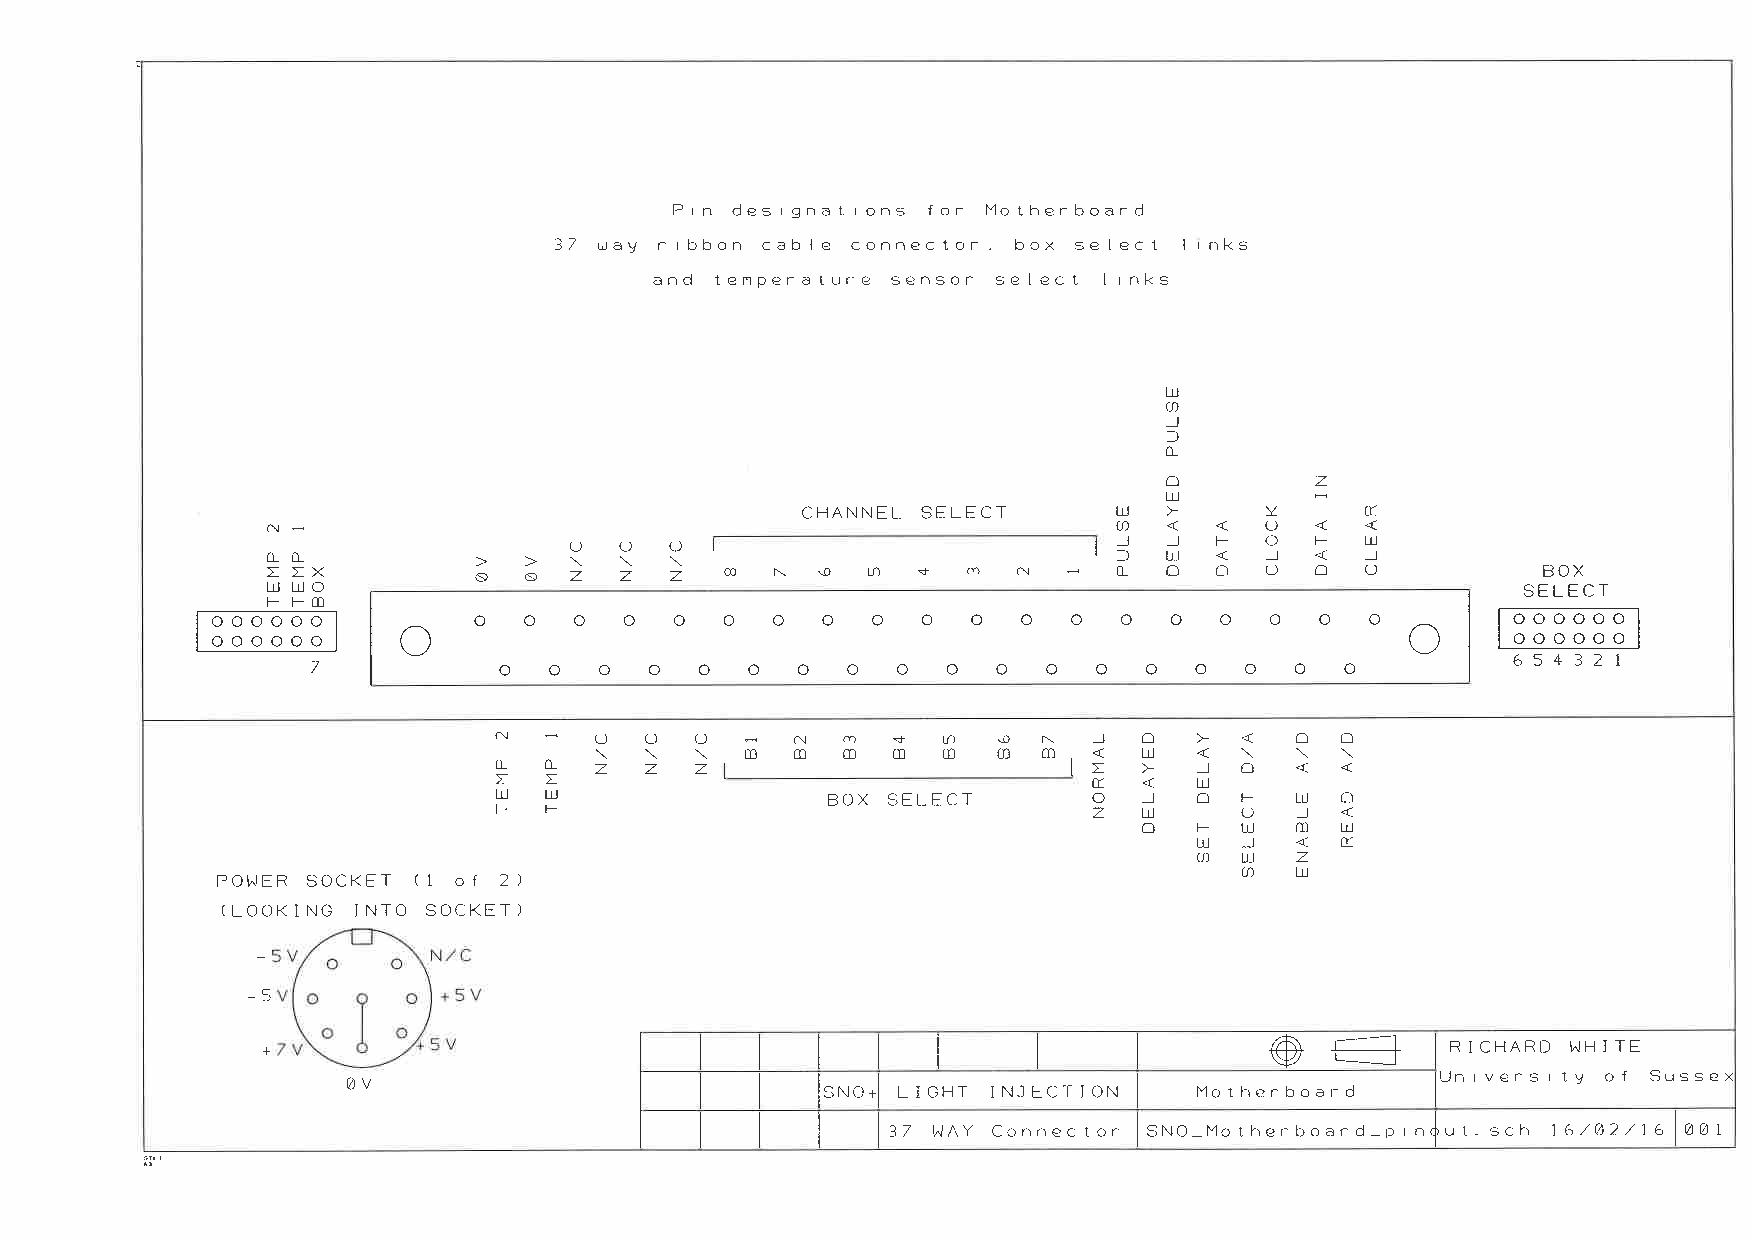
\includegraphics[width=0.85\textwidth]{LEDBoxMotherboard}
		\caption{A schematic showing of the pin input connections on an LED driver box motherboard. }
		\label{fig:LEDBoxMotherboard}
	\end{center}
\end{figure}

\section{The TELLIE LED}
\label{sec:LEDcoupling}

For the purposes of TELLIE there are two vital characteristics to consider when identifying candidate LEDs: the time profile of the LED pulse be as short as possible and the wavelength so be chosen to minimise scattering in the scintillator volume. These parameters are discussed in the following sections. 

The LED selected in the TELLIE system os a BL-LUCY5N15C from Bright LED. It has a peak emission wavelength of 505~nm and a differential resistance of only 10 $\Omega$ in the linear region of forward current against forward voltage when operating above the LED threshold. Typically, the resistance of a LED is between 40 and 100 $\Omega$. 

\subsection{LED time profile}

For the purposes of TELLIE it is vital that the time profile of the LED pulse be as short as possible. In order to identify what type of electrical characteristics a candidate LED should have we can use an approximation of LED modulation characteristics. In this approximation the LED is described as an active region of volume $V_a$ driven by a constant forward current $I_f$ switched on at t = 0. Electrons are injected into $V_a$ increasing the carrier concentration $n_a$. The emitted rate of photons per volume is $dn_{\gamma}/dt = n_a/\tau_e$ where $\tau_e$ is the average time for a charge carrier to recombine and generate a photon. For a constant $I$, which switches on instantaneously once the voltage across the LED reaches a threshold, thus neglecting the large stationary charge densities either side of the LED's active region and their inherent capacitance, the emitted rate of photons is: 

\begin{equation}
\frac{dn_\gamma}{dt} (t) = I_f \cdot  \frac{1}{eV_a} \cdot \frac{\tau_l}{\tau_e} \cdot \bigl( 1 - e^{- \frac{t}{\tau_l} } \bigr)
\label{eq:LEDBrightness}
\end{equation}

Here $\tau_l$ is the average time for a charge carrier to be lost from the active volume and $e$ is the charge on an electron. $\tau_l$ and $\tau_e$ are intrinsic to the pn-junction and are not variable. Therefore, Equation~\ref{eq:LEDBrightness} implies that the current through the pn-junction is critical for the time to reach a desired photon emission rate, i.e., increasing the current will reduce the rise time. A similar argument applies for the fall time on application of a reverse current $I_r$: applying a current in reverse bias, sweeps charge carriers away from $V_a$, reducing the fall time of the LED light pulse. The limiting factor to the amount of current that can be applied to an LED is its resistance. \textbf{The resistance is therefore the most important parameter to consider when seeking an optimal time profile.}

\subsection{Spectral constraints}
As the Rayleigh scattering of a medium quickly drops with increasing wavelength, the LEDs should have the highest possible peak wavelength to optimise direct transmission. However, the wavelength must be selected in the context of the system which will detect it, i.e. the quantum efficiency of the PMTs, which drops quickly at higher wavelengths. Given the expected absorption spectrum of the Te doped LAB-based scintillator and the quantum efficiency of the SNO+ PMTs, the optimal peak wavelength is close to 500nm. These spectra, together with the measured wavelength distribution of the selected LEDs are shown in Figure~\ref{fig:LEDWavelength}.

\begin{figure}[htbp]
	\begin{center}
		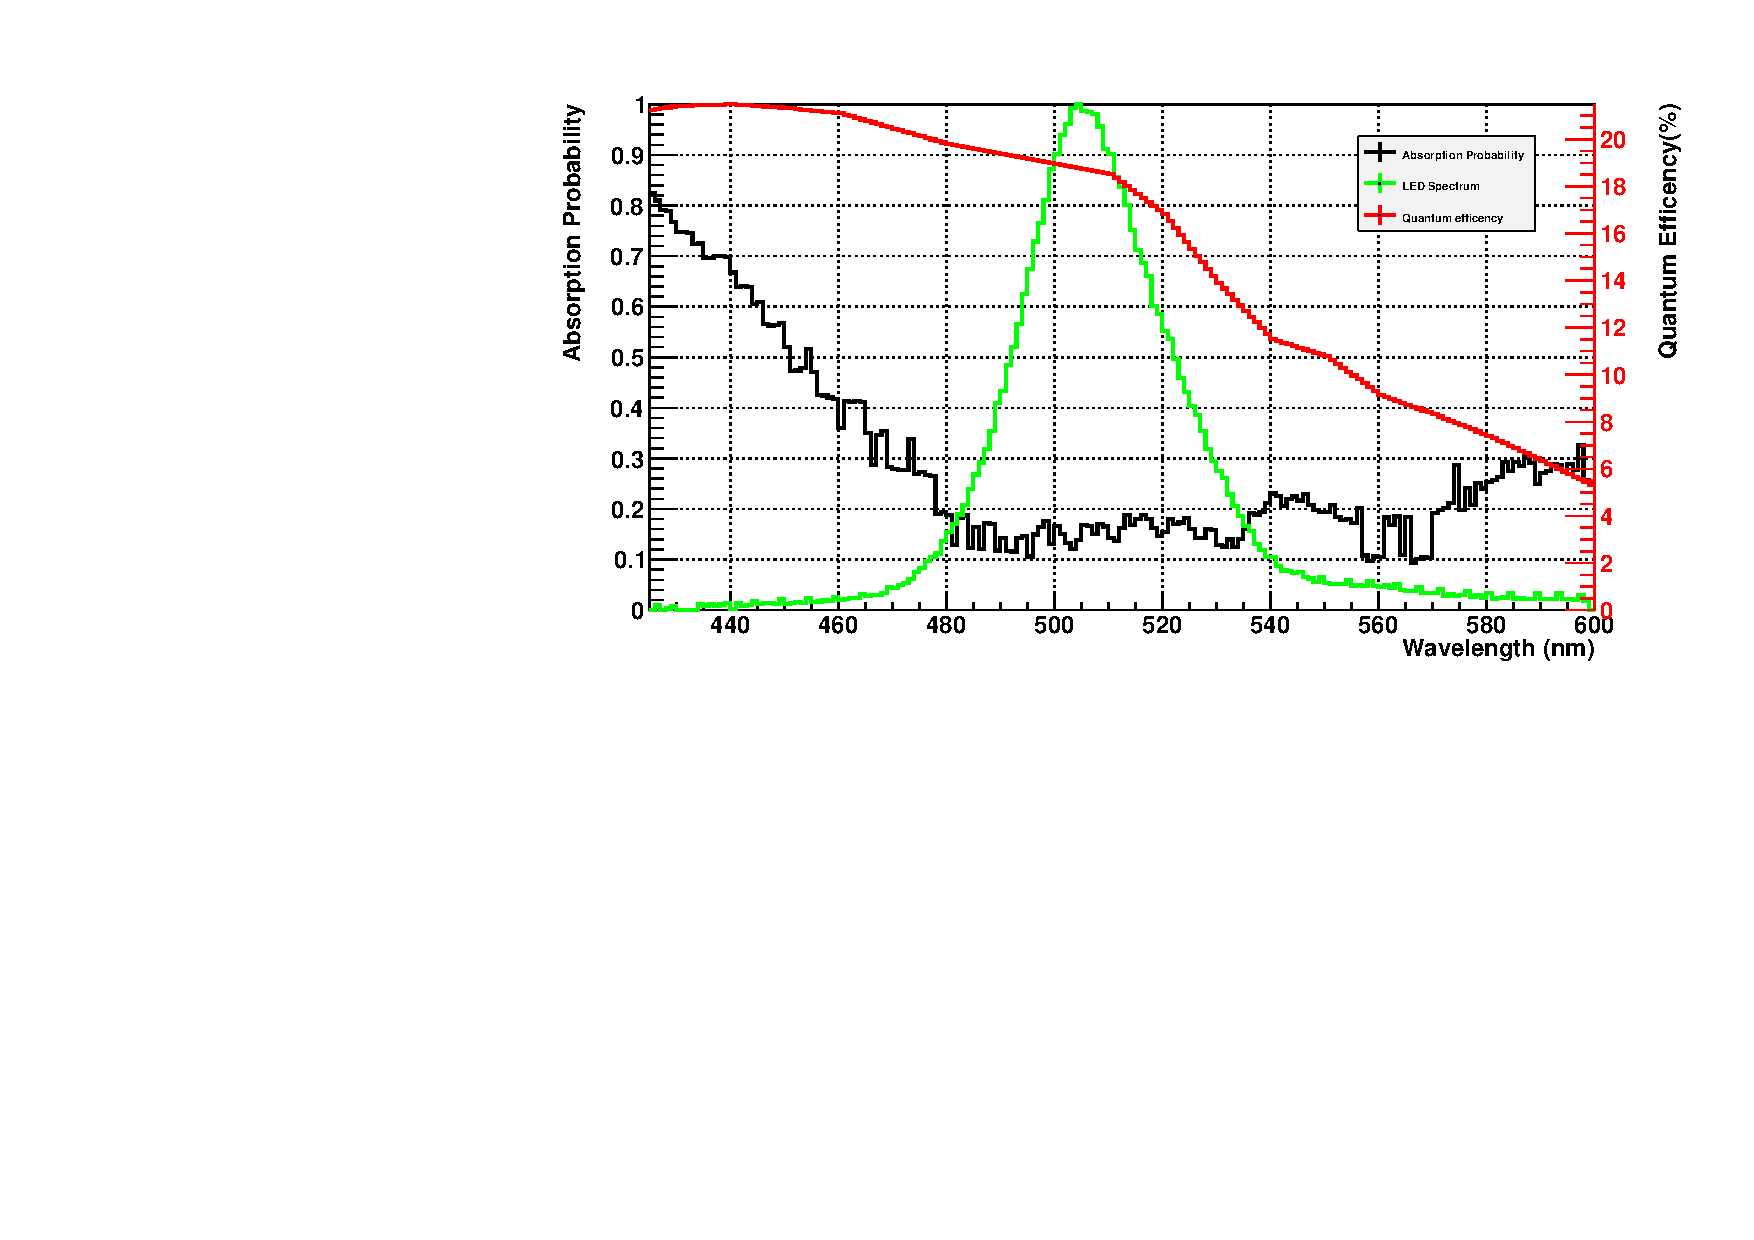
\includegraphics[width=0.7\textwidth]{LEDWavelength}
		\caption{The absorptions probability spectrum of $^{130}$Te doped LAB and PPO (black), the average spectrum for all 96 LEDs as measured at Sussex (green), in arbitrary units, and the SNO+ PMT quantum efficiency (red).}
		\label{fig:LEDWavelength}
	\end{center}
\end{figure}

\subsection{LED Coupling}
\label{subsec:LEDCoupling}
In order to maximise the optical transmittance between the LED and optical fibre used to couple the light out each LED was hand drilled to provide a socket into which an optical fibre of 1~mm diameter was fixed, see Figure~\ref{fig:LEDCoupling}a. The fibre tip was nominally 1~mm from the LED's diode chip. An index match optical glue was used to secure the fibre in the socket [WHICH GLUE??].

To provide a light tight environment for the PIN diodes, as well as some amount of mechanical stability, the coupled LED and fibre are contained within a brass ``cone'', see Figure~\ref{fig:LEDCoupling}b. The PIN diode is mounted into the opposite side of the cone from the LED and monitors light intensity produced in an emission event. The digitised output from the photodiode transmitted back to the control box via the ribbon cable attached to the front of the driver box for processing. 

\begin{figure}
	\centering
	\subfloat[]{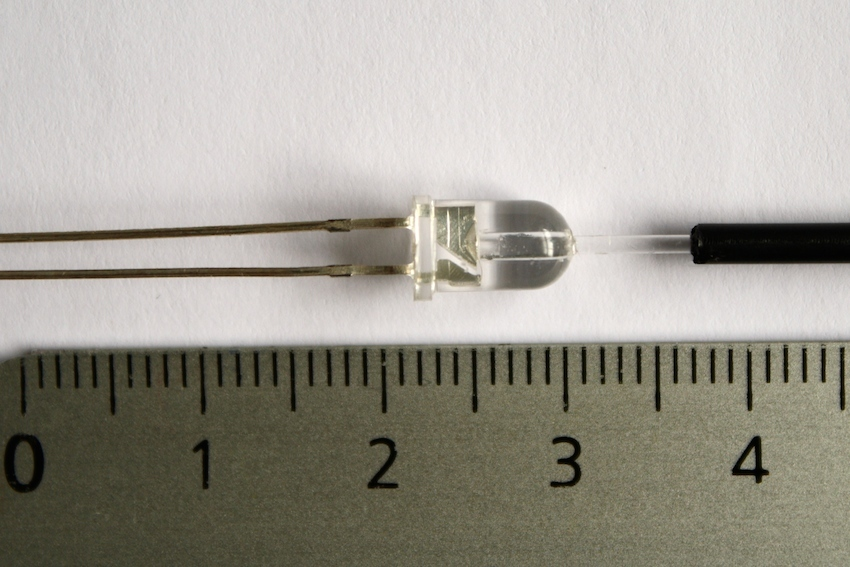
\includegraphics[width=0.53\textwidth]{LEDDrilled}} 
	\subfloat[]{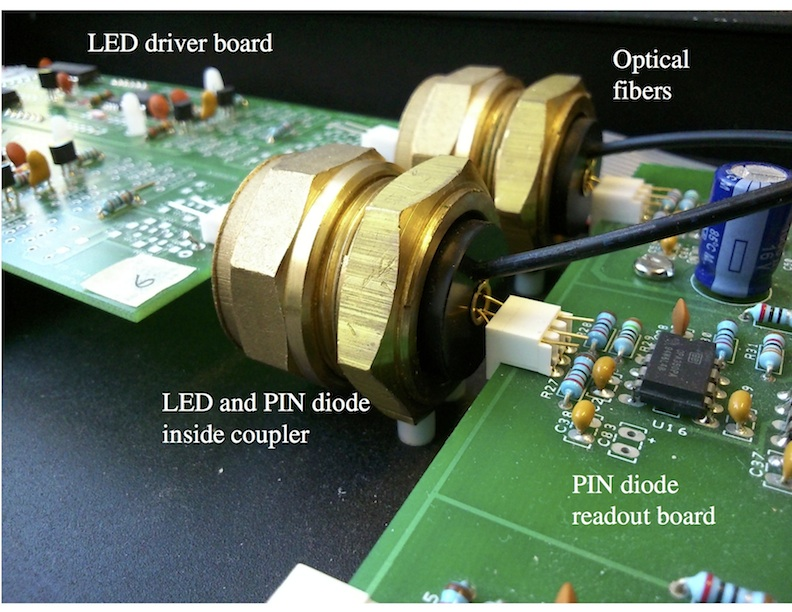
\includegraphics[width=0.47\textwidth]{LEDcoupler}}
	\caption{(a) Drilled LED with coupled optical fibre (ruler in cm). (b) Brass ``cone'' coupling device containing LED and photodiode to monitor the number of photons at injection.}
	\label{fig:LEDCoupling} 
\end{figure}


\section{Push pull LED drivers}
\label{sec:LEDdrivers}
The push pull LED drivers implemented in the TELLIE system were developed in a collaborative effort between the Universities of Sussex and Leeds. The designed is based around a commercially available laser diode driver, the IXLD02SI from IXYS Colarado. The IXLD02 is sold as an ultra high-speed differential laser diode driver designed to drive single junction diodes. 

The IXLD02 does not provide any voltage or current, rather it sinks current by manipulating output sink MOSFETs in a linear manner. The resistance of the MOSFETs are used, along with external resistor banks to form two potential dividers, one at the anode and one at the cathode of an LED. To maintain a nominal reverse and forward bias, the external resistances are optimised relative to the resistance of the MOSFETs, setting the maximum current that can be delivered to the LED. 

The driver circuit, shown in Figure~\ref{fig:IXDX02_circuit}, operates by briefly flipping the voltage across the LED to a forward voltage and then back to a reverse. Initially transistor $Q_1$ is open and transistor $Q_2$ is closed. To allow a forward voltage across the LED, $Q_1$ closes and $Q_2$ opens. In switching the LED off, returning $Q_1$ and $Q_2$ to their initial states creates a temporary reverse current, which sweeps charge carriers from the LED's active region - reducing the fall time of the LED pulse. Resistor bands $R_1$ and $R_2$ serve to limit the current through $Q_1$ and $Q_2$ as well as generating sufficiently large forward and reverse voltages across the LED. $Q_1$ and $Q_2$ form part of the integrated circuitry (IC) of the IXLD02SI driver, the driver also contains the MOSFET drivers and the circuits to set the pulse width and pulse amplitude, using currents: Pulse Width ($I_{PW}$) and Operational ($I_{OP}$) respectively. LED pulses are triggered via the trigger (TRIG) input, between each pulse the current through $Q_1$ or $Q_2$ can be powered down via the Power Down (PDN) input. 

\begin{figure}[htbp]
	\begin{center}
		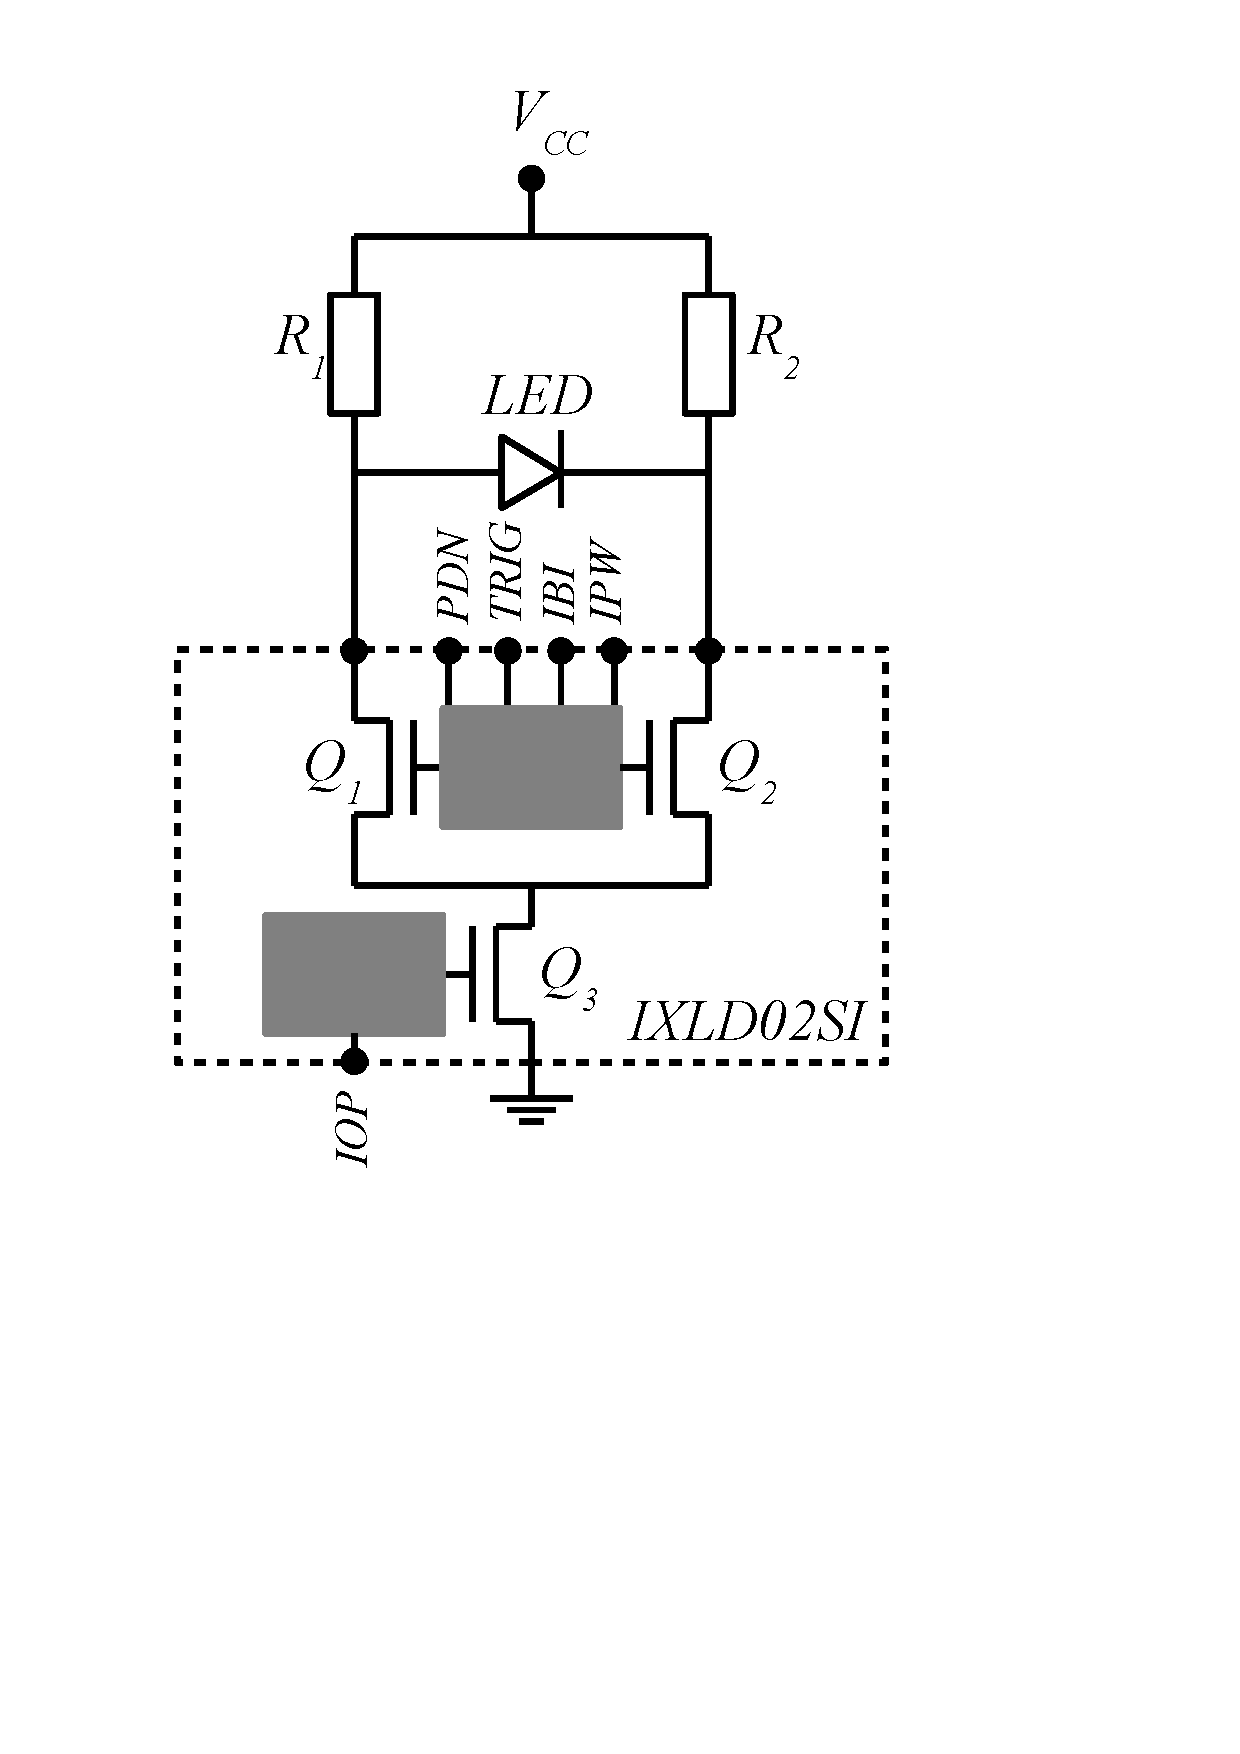
\includegraphics[width=0.4\textwidth]{ixld02_circuit}
		\caption{The driver circuit based on the IXLD02SI chip. Only main components are shown, the rest of the integrated circuit is represented with grey boxes.}
		\label{fig:IXDX02_circuit}
	\end{center}
\end{figure}

\begin{figure}[htbp]
	\begin{center}
		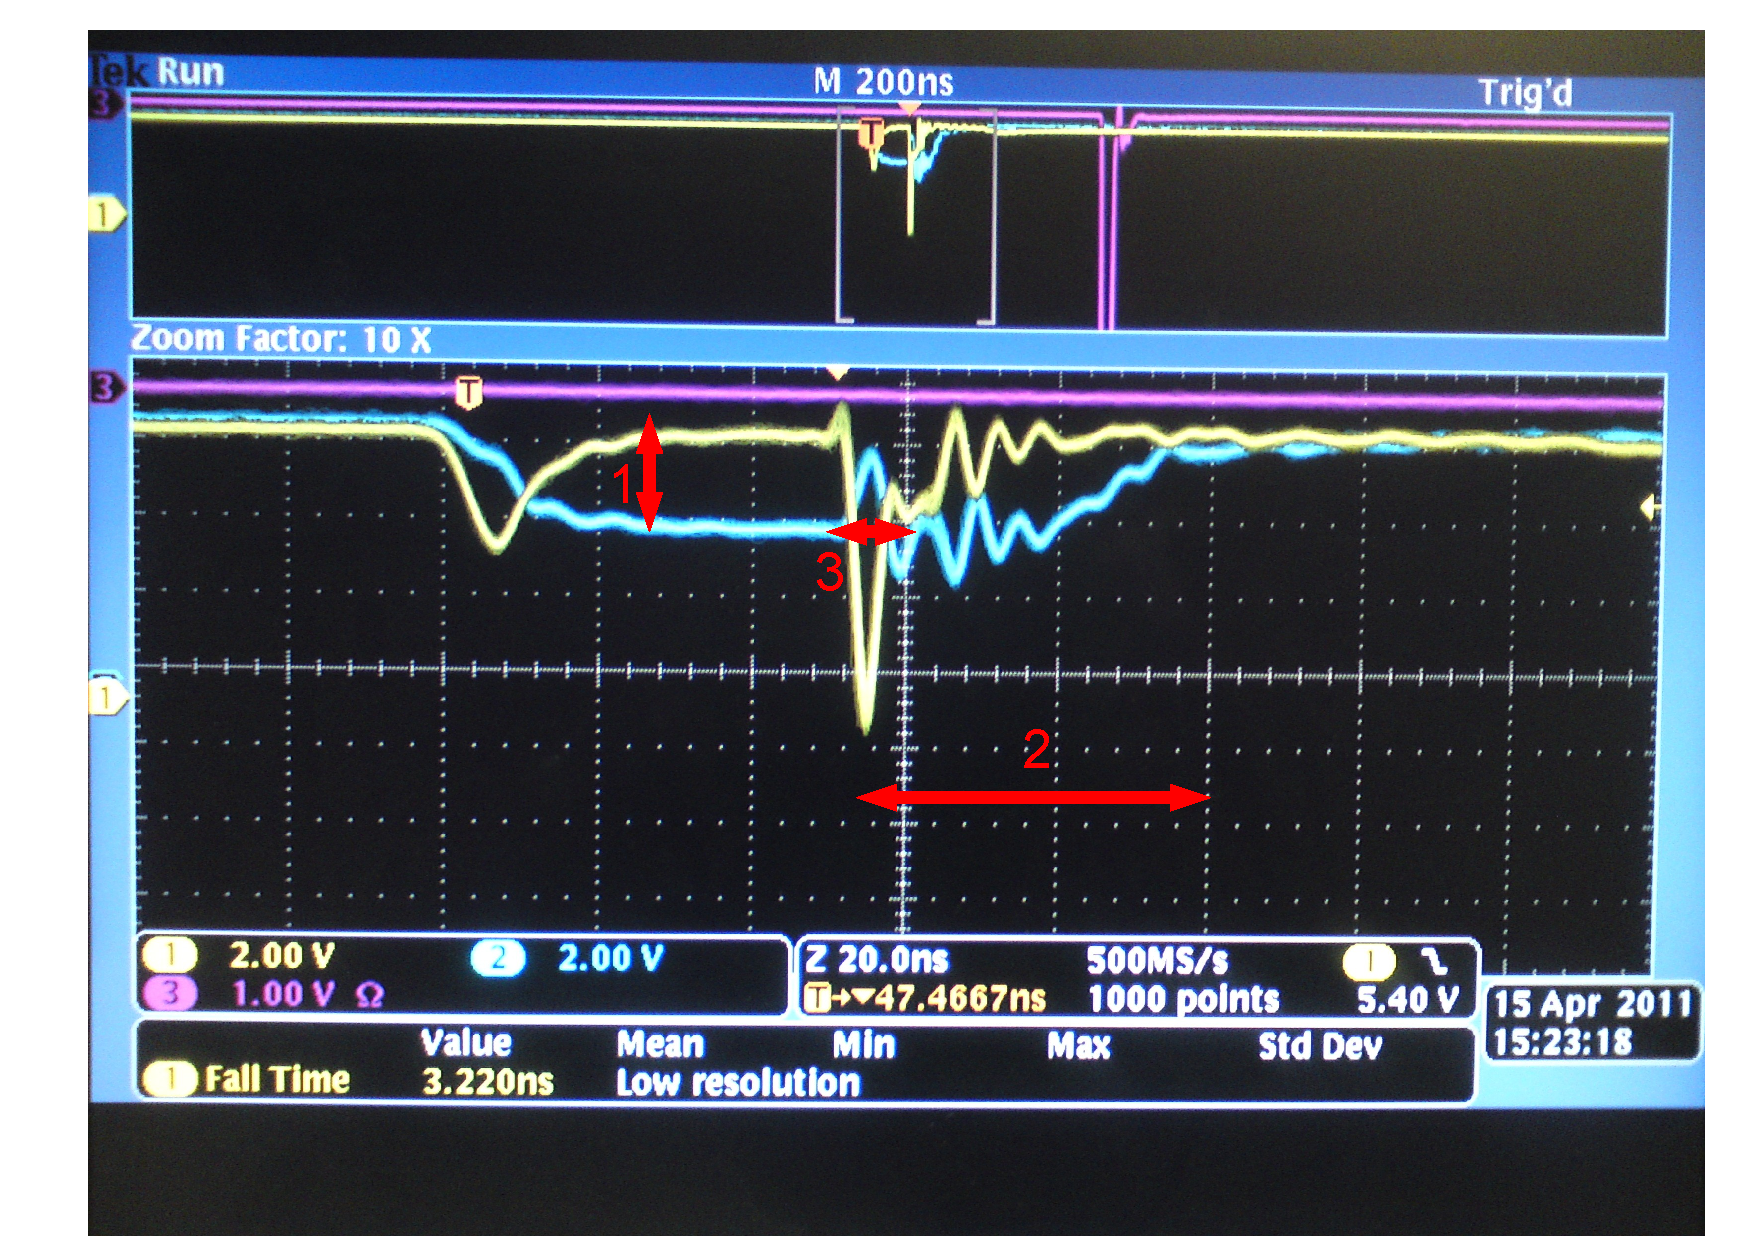
\includegraphics[width=0.6\textwidth]{driver_voltages}
		\caption{The voltages as measured at the anode (blue) and cathode (yellow) of the LED, the ringing is due to impedance miss matches at the probes. $I_{OP}$ sets the maximum bias applied to the LED (1); the bias current $I_{BI}$ sets the maximum length of time that the voltages at the anode and cathode of the LED can be inverted (2); $I_{PW}$ sets the time that the voltages are inverted (3)}
		\label{fig:LEDDriverScope}
	\end{center}
\end{figure}


The three adjustable parameters are: 
\begin{itemize}
	\item $I_{OP}$: activates the chip and sets the maximum bias applied to the LED and in turn the maximum pulse amplutude.
	\item $I_{BI}$: sets the maximum length of time that the voltages at the anode and cathode of the LED can be inverted i.e. the maximum possible pulse width.
	\item $I_{PW}$: sets the time that the voltages are inverted, i.e. the resulting pulse width.
\end{itemize}

If $I_{PW}$ = $I_{BI}$, the pulse width is 0. As $I_{PW}$ approaches $I_{BI}$ but is less than $I_{BI}$, the pulse width becomes nonzero. 

The IXLD02SI has no internal protection against over-heating. Two methods are used to protect the driver: a 50~mA fuse and an upper limit of 100 kHz on the trigger rate. In addition, during the development phase several drivers were damaged by noise on the trigger and the fuse being too slow. To further protect the drive the power supply ($V_{CC}$ in Figure~\ref{fig:IXDX02_circuit}) is restricted to 7~V and 30~mA. 

\subsection{Board designs \& description}
This section is currently just a place holder. The included schematic is a little out of date. Richard White at Sussex is working on a full write up for this section. 

\begin{figure}[htbp]
	\begin{center}
		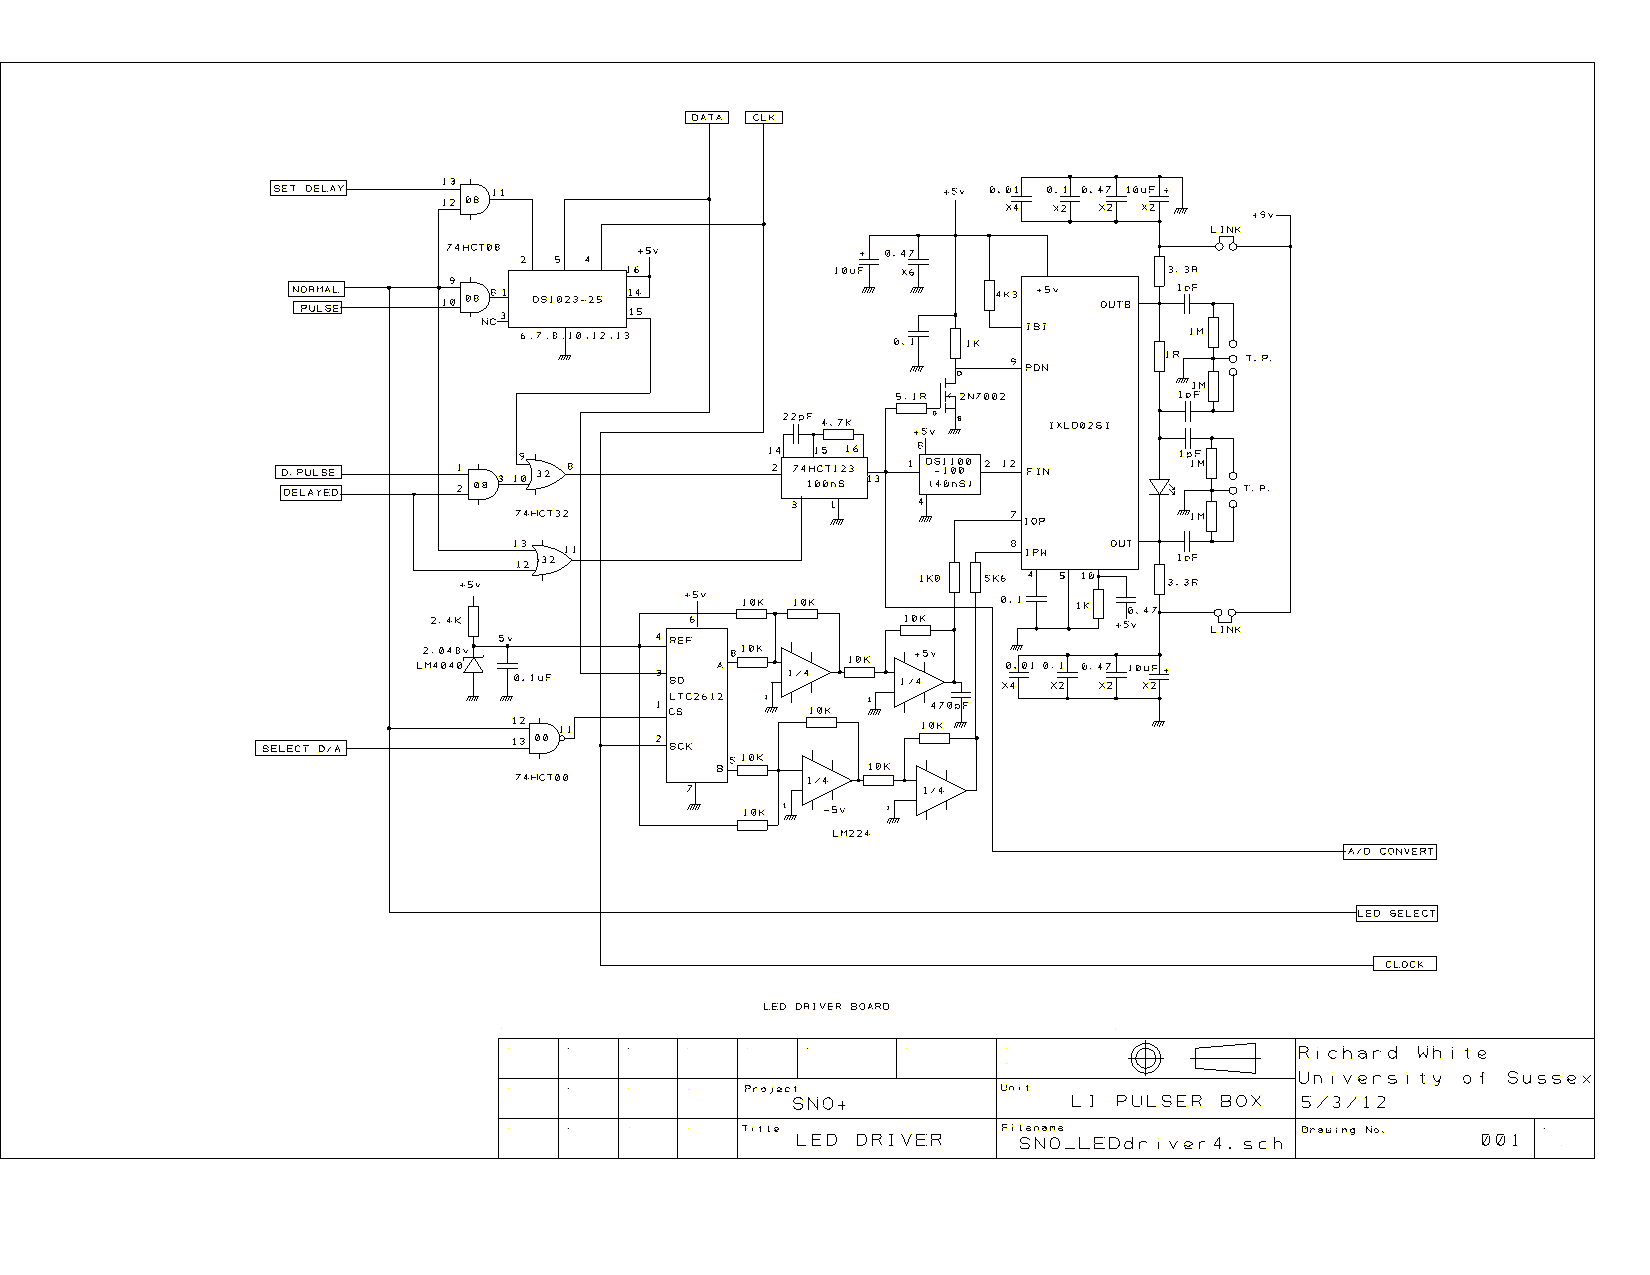
\includegraphics[width=1.0\textwidth]{LEDDriverSchematic}
		\caption{Schematic design of the LED driver circuit.}
		\label{fig:LEDDriverSchematic}
	\end{center}
\end{figure}


\subsection{Performance}
\label{subsec:DriverPerformance}
\subsubsection{Timing performance}
Measurements of the optical time profile of TELLIE's LED driver system were made with 45~m of optical fibre connecting the driver and LED to a readout PMT, to mimic the optical path into the SNO+ detector. The time profiles for the IXLDO2SI driver operating at 10~kHz with pulse intensities of 10$^3$ and 10$^6$ photons per pulse are shown in Figures \ref{fig:DriverProfile_1e3} and \ref{fig:DriverProfile_1e6} respectively. Great effort was put into minimising systematic contributions of the measurement system to the resulting time profile. For full details see James Sinclair's thesis \cite{Sinclair}. 

\begin{figure}[htbp]
	\begin{center}
		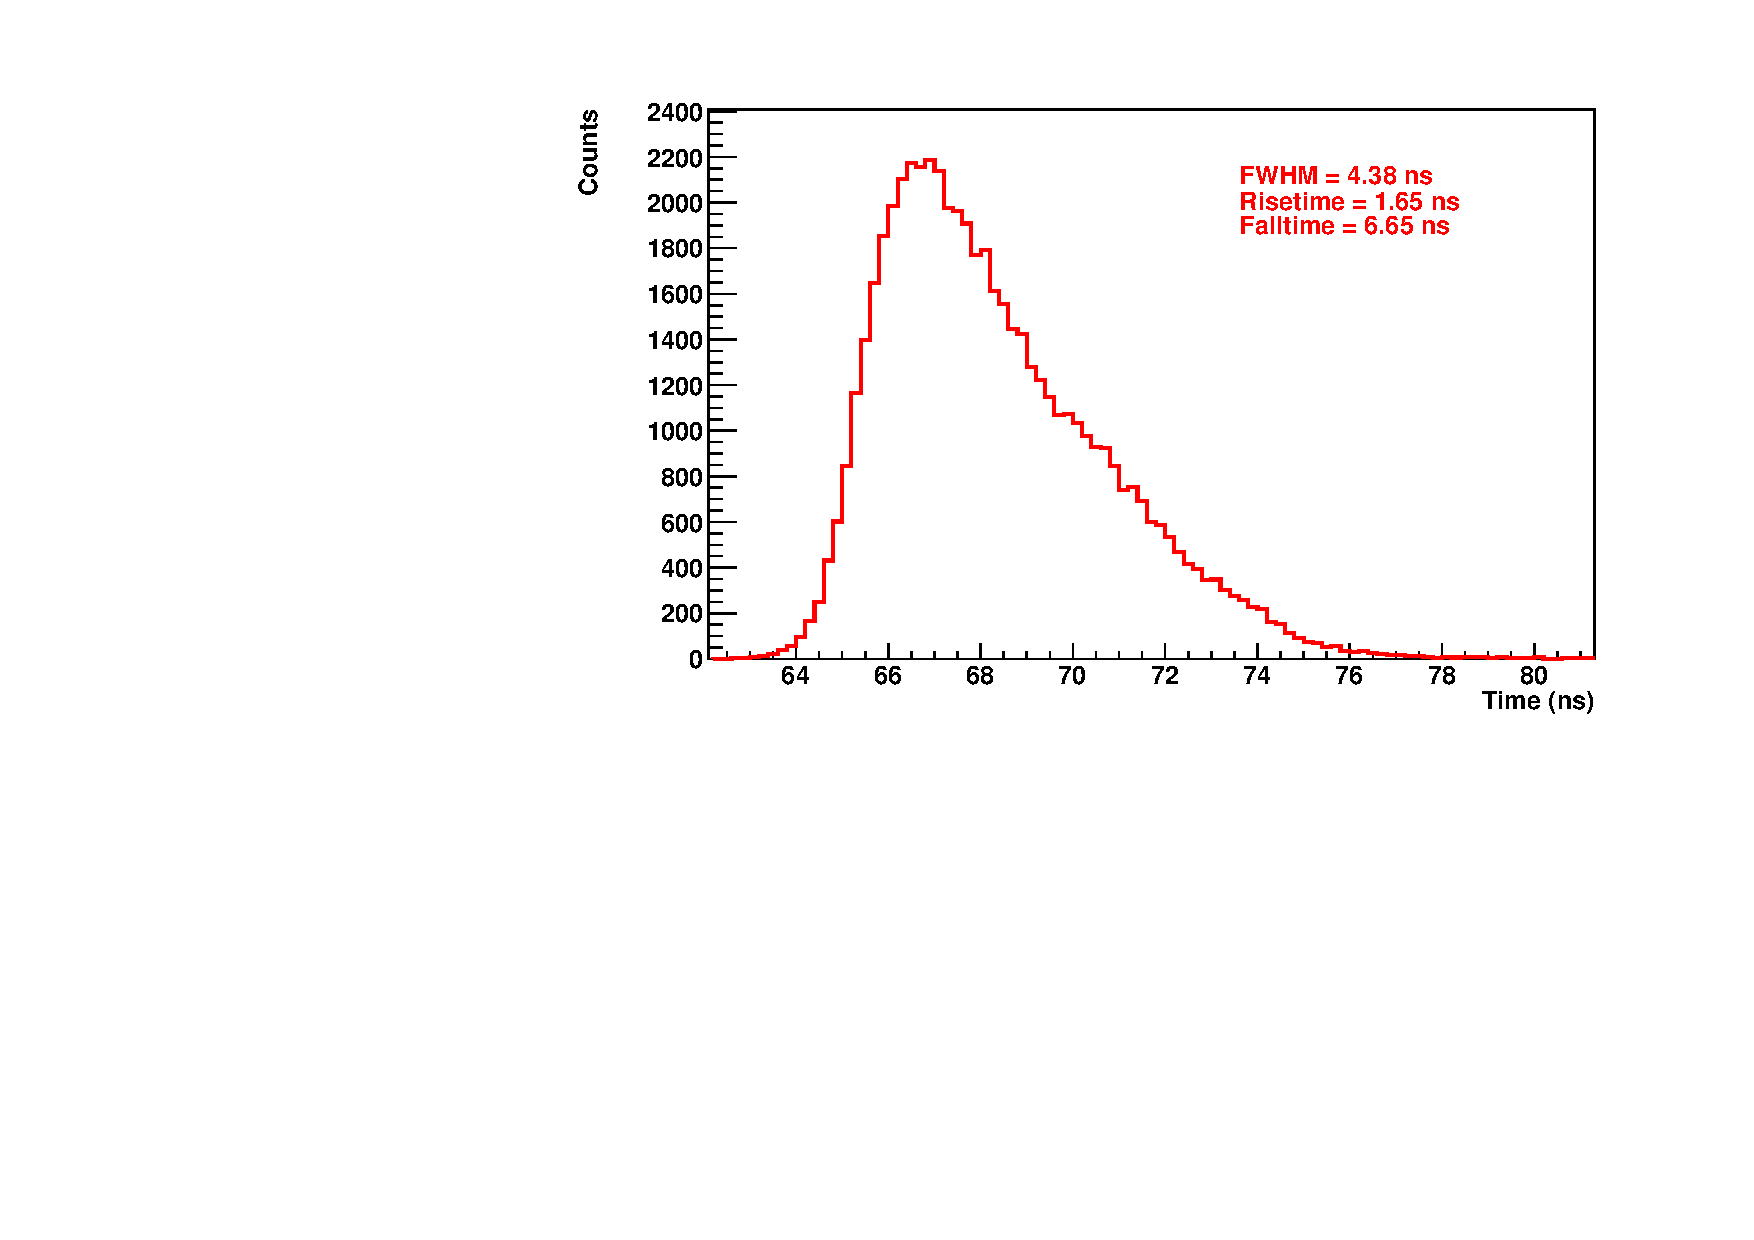
\includegraphics[width=0.6\textwidth]{DriverProfile_1e3}
		\caption{The time profile for the TELLIE push pull driver at a pulse intensity of 10$^3$ photons per pulse, running at 10~kHz. For the measurement, the driver and LED were connected to the PMT via 45~m + 0.75~m = 45.75~m of optical fibre.}
		\label{fig:DriverProfile_1e3}
	\end{center}
\end{figure}

\begin{figure}[htbp]
	\begin{center}
		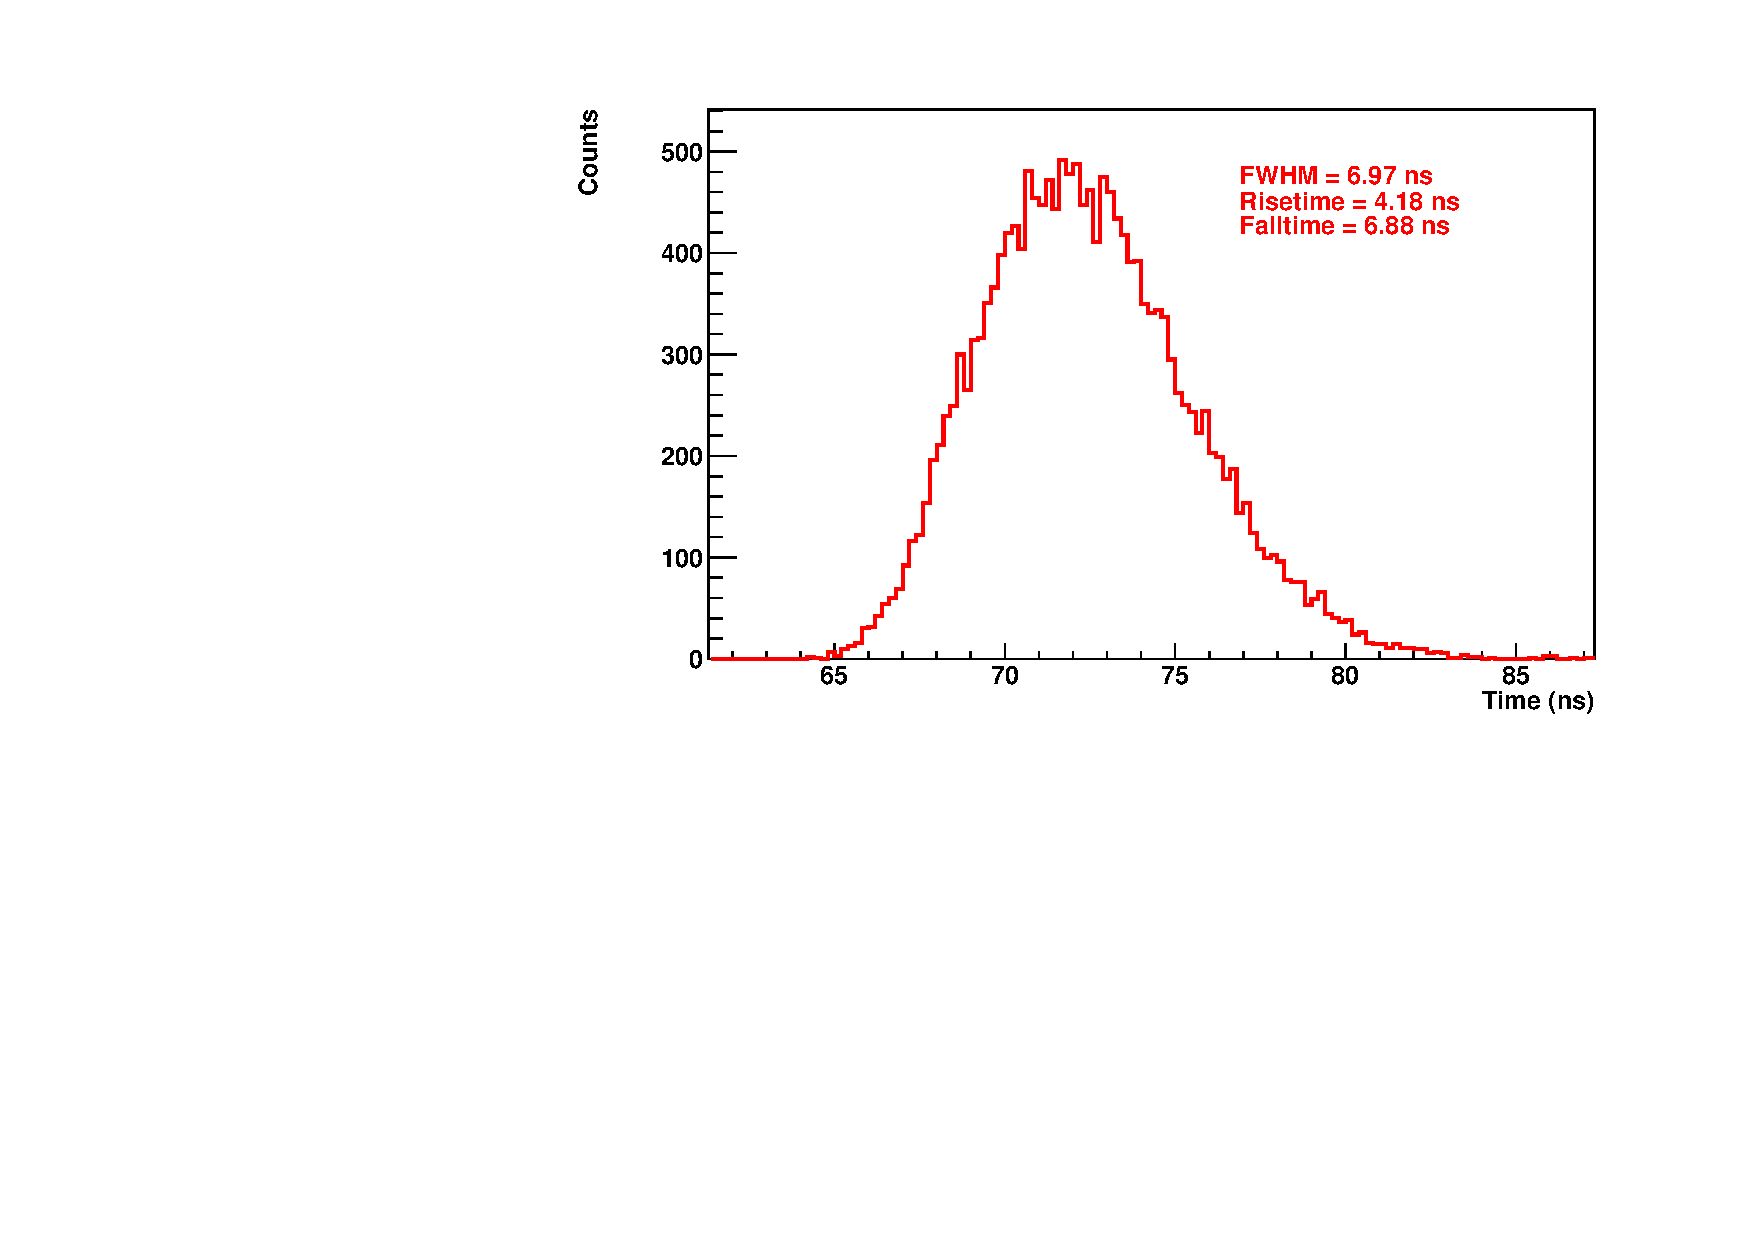
\includegraphics[width=0.6\textwidth]{DriverProfile_1e6}
		\caption{The time profile for the TELLIE push pull driver at a pulse intensity of 10$^6$ photons per pulse, running at 10~kHz. For the measurement, the driver and LED were connected to the PMT via 45~m + 0.75~m = 45.75~m of optical fibre.}
		\label{fig:DriverProfile_1e6}
	\end{center}
\end{figure}

The results of the characterisation of one driver's output is shown in Table~\ref{tab:ixld}, a summary of the time profiles for four different amplitudes. A broadening of the pulse at higher intensities is observed. These measurements were made with the long fibre coiled in a bundle, ensuring mode mixing. The results shown here are for only one driver, the variation across the entire system is measured in the channel-to-channel calibrations performed at SNOlab (shown in Figure~\ref{fig:IntensitySweeping}), however these measurements don't account for the temporal response of either the benchtop PMT or oscilloscope used to read it out. This adds significant systematics to the measurement and broadens the measured response. 

\begin{table}[t]
	\centering
	\begin{tabular}{| c | c | c | c |}
		\hline                        
		Number of Photons & Full Width Half Maximum (ns) & Rise Time (ns) & Fall Time (ns) \\ \hline \hline
		$10^{3}$ & $4.4$   & $1.6$ & $6.6$\\ \hline
		$10^{4}$ &$4.4$   & $2.0$ & $6.0$\\ \hline
		$10^{5}$ &$5.2$   & $2.0$ & $6.4$\\ \hline
		$10^{6}$ &$7.0$   & $4.2$ & $6.8$\\ \hline
	\end{tabular}
	\caption{Summary of time profile measurements for a single LED and driver at varying intensities. 
			All measurements made with the driver running at 1\,kHz. The measurement of the number of photons is performed after 45.75\,m of optical fibre, i.e., not including the 2\,m patch cord.}
	\label{tab:ixld} 
\end{table}

\subsubsection{Angular response}
The emission profile of the fibres was measured using a custom designed experimental arrangement at Sussex. A x-y stage was used to scan the surface normal to the optical emissions from a fixed fibre. A push pull driver, as described above, was used to inject light into a 2~m patch cable and onwards into a 45~m cable to reproduce the connections in the final system. The PMT had its optical acceptance window covered by a plate with a 1~mm diameter hole, limiting the effective detecting area. Intensity measurements were then taken at incremental points within the plane. Further details on the experimental arrangement can be found in \cite{Sinclair}. 

The 2D map of coincidences between PMT and LED driver is corrected for accidental coincidences and the geometry of the set-up. It is then converted into an angular intensity map in water, shown in Figure~\ref{fig:AngularResponse}. The fraction of the total light emitted within a cone of 14.5$^{\circ}$ (in air) from the centre is found to be 80\%\footnote{given the refractive index of air and water, and the numerical aperture of the fibre, 14.5$^{\circ}$  in air corresponds to 11$^{\circ}$ in water}. The visible asymmetry about the central point in Figure~\ref{fig:AngularResponse} is likely due to the way the fibre was mounted in the duplex termination point; a metal band was used to clamp the fibre just before this point, effectively flattening it a little. 

\begin{figure}[htbp]
	\begin{center}
		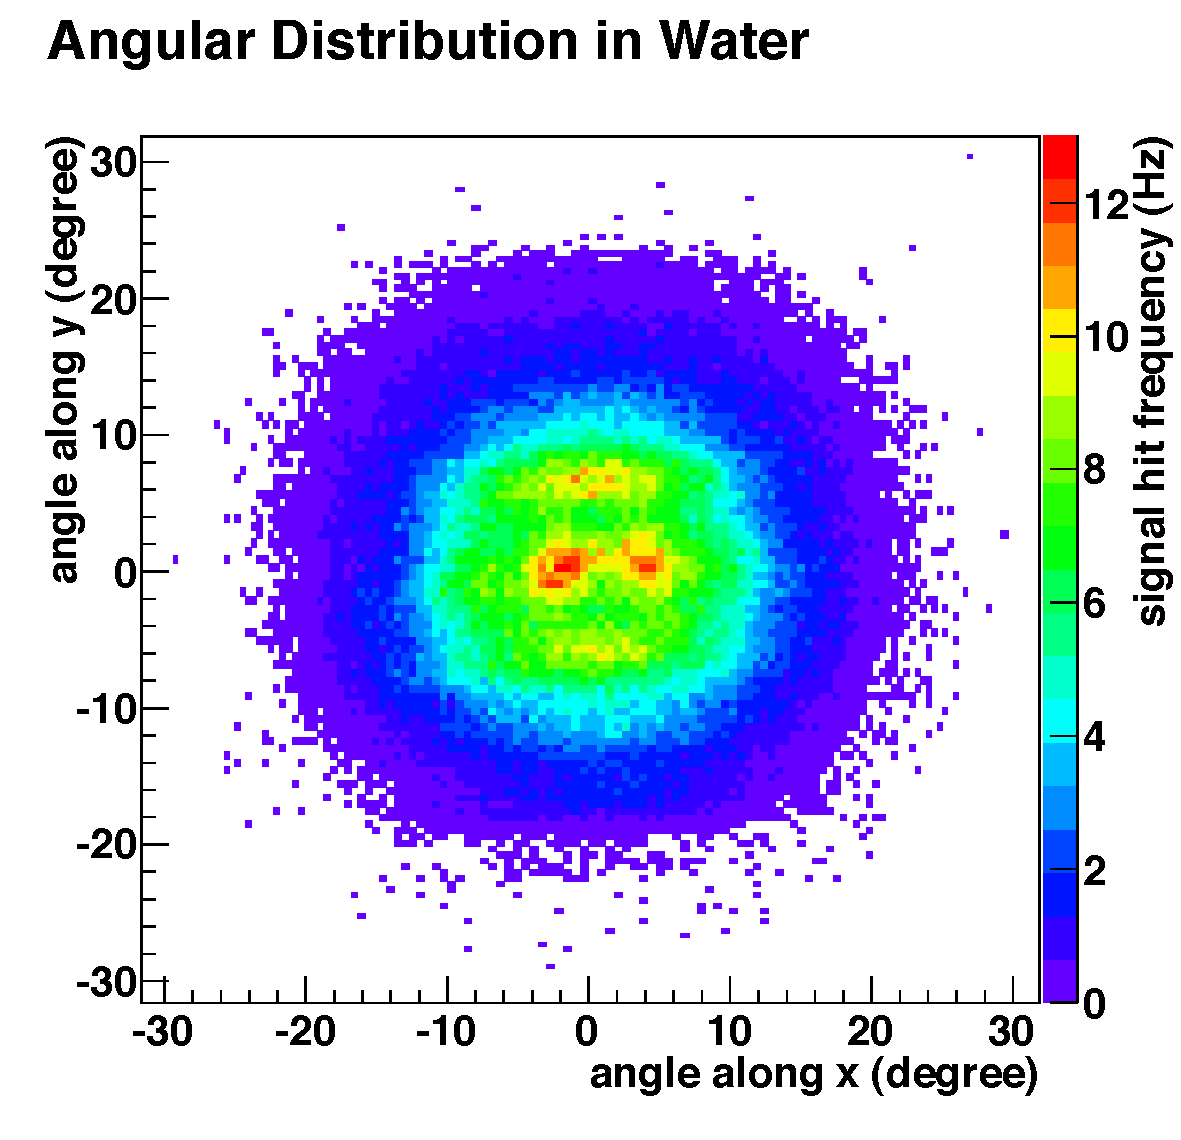
\includegraphics[width=0.6\textwidth]{AngularResponse}
		\caption{Two dimensional angular emission profile of a fibre. The while area corresponds to zero intensity. The steps in x and y are fixed during the measurement, hence the variable angular resolution, ranging from 0.6$^{\circ}$ to the centre to 0.26$^{\circ}$ at the edges.}
		\label{fig:AngularResponse}
	\end{center}
\end{figure}

\subsubsection{Intensity response}
At the time of writing, the intensity response of each of TELLIE's 96 channels has been calibrated for master mode operation. Experimentally these measurements were taken using a variable gain PMT calibrated over its operational range. A low gain measurement was taken to map the full intensity range of the driver board. A high gain measurement is then taken to characterise the low intensity range. 

The results of both high and low sweep measurements for a single PMT are shown in Figure~\ref{fig:IntensitySweeping}. Each figure includes four plot; the photon output, as measured by the calibrated benchtop PMT, as a function of IPW. Pulse shape measurements as a function of IPW. The PIN diode read out as a function of IPW and, finally, PIN doiode response as a function of photon output.

\begin{figure}
	\centering
	\subfloat[Full intensity range]{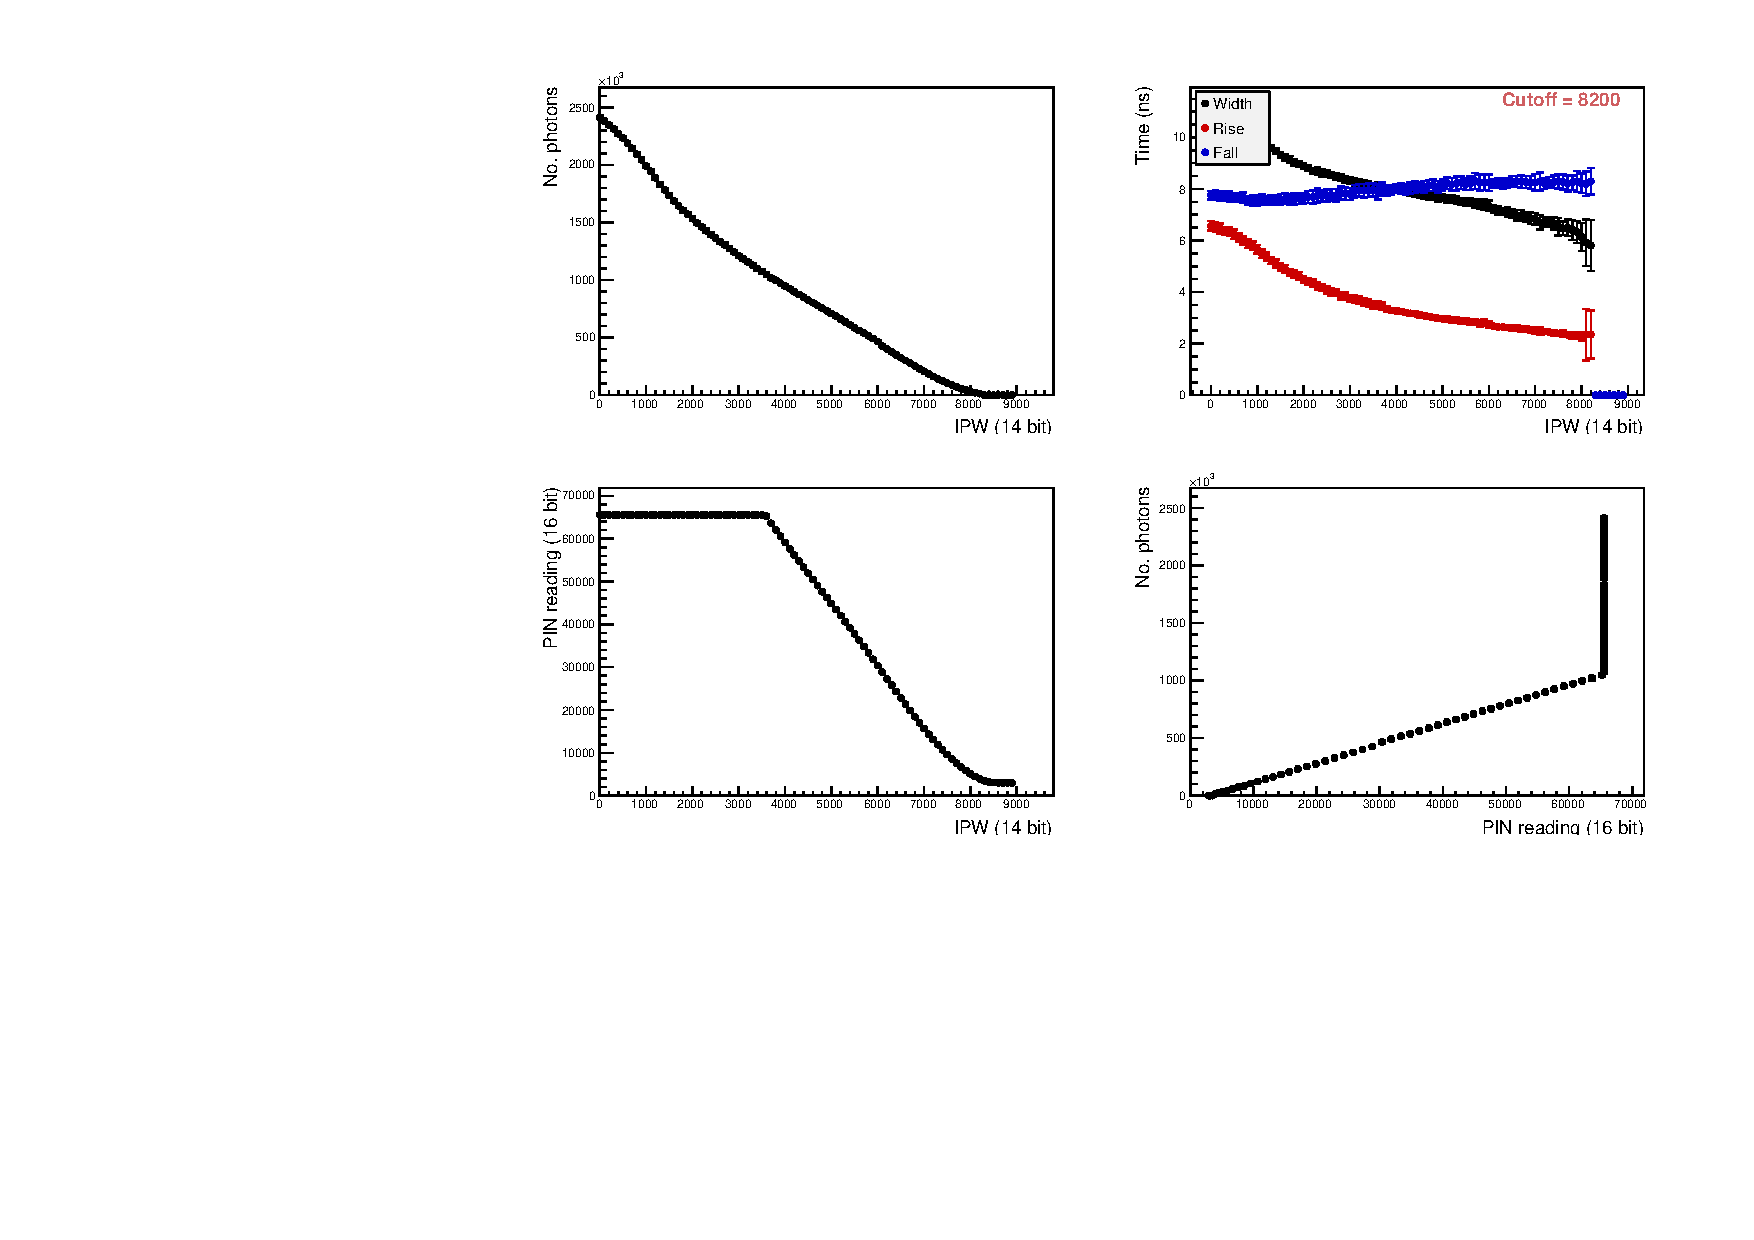
\includegraphics[width=0.50\textwidth]{IntensityBroadSweep}} 
	\subfloat[Low intensity range]{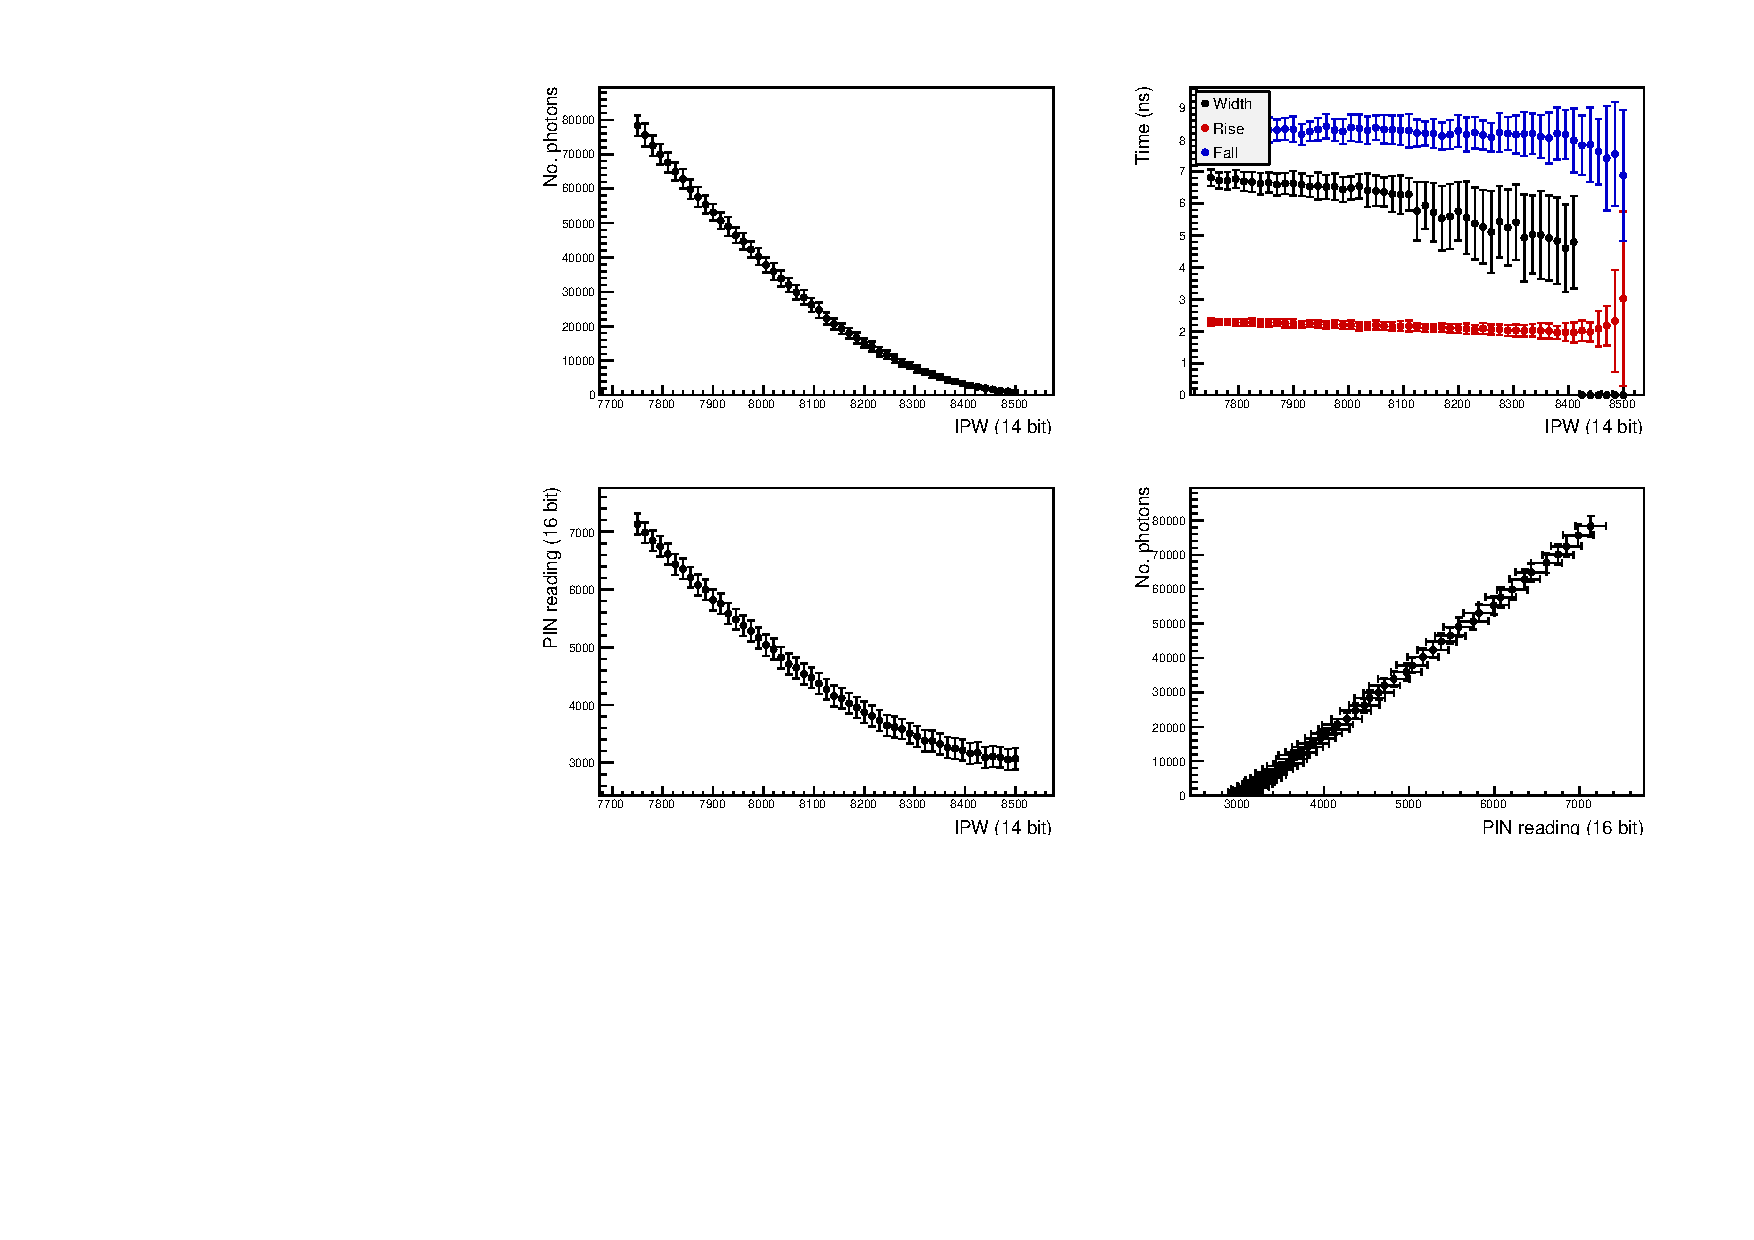
\includegraphics[width=0.50\textwidth]{IntensityLowSweep}}
	\caption{Plots taken from Master mode calibrations of TELLIE for both the full operational range and a more detailed low intensity region where most of TELLIE's work will be done.}
	\label{fig:IntensitySweeping} 
\end{figure}

\section{PIN diode light intensity monitoring}
\label{sec:PIN}
As described in section~\ref{subsec:LEDCoupling}, PIN diodes are installed in the LED `cones'. Any light which does not couple into the Fibre illuminates the inside of the cone. The PIN's response is amplified through a chain of two op-amps, described in the following section ~\ref{subsec:PINDesigns}. A 14 bit digitizer then measures the signal and communicates it back to the control box as a digital number. 

The gain of the op-amp chain and the pick off point can be adjusted by two potentiometers on the boards, shown in Figure~\ref{fig:PINDiodePots}a. Here, POT 1 controls the ADC's sample point (the blue edge shown in Figure~\ref{fig:PINDiodePots}b) and POT 2 the gain applied by the amplifier read out chain (the amplitude of the yellow trace in Figure~\ref{fig:PINDiodePots}a). By adjusting these two POTs the PIN diodes response can be tuned to be more or less sensitive. Full procedures outlining exactly how the PIN diode response was optimised for low light levels are detailed in \cite{tellieCalibProceedures}. 

\begin{figure}
	\centering
	\subfloat[POTs and probe connection points for PIN diode]{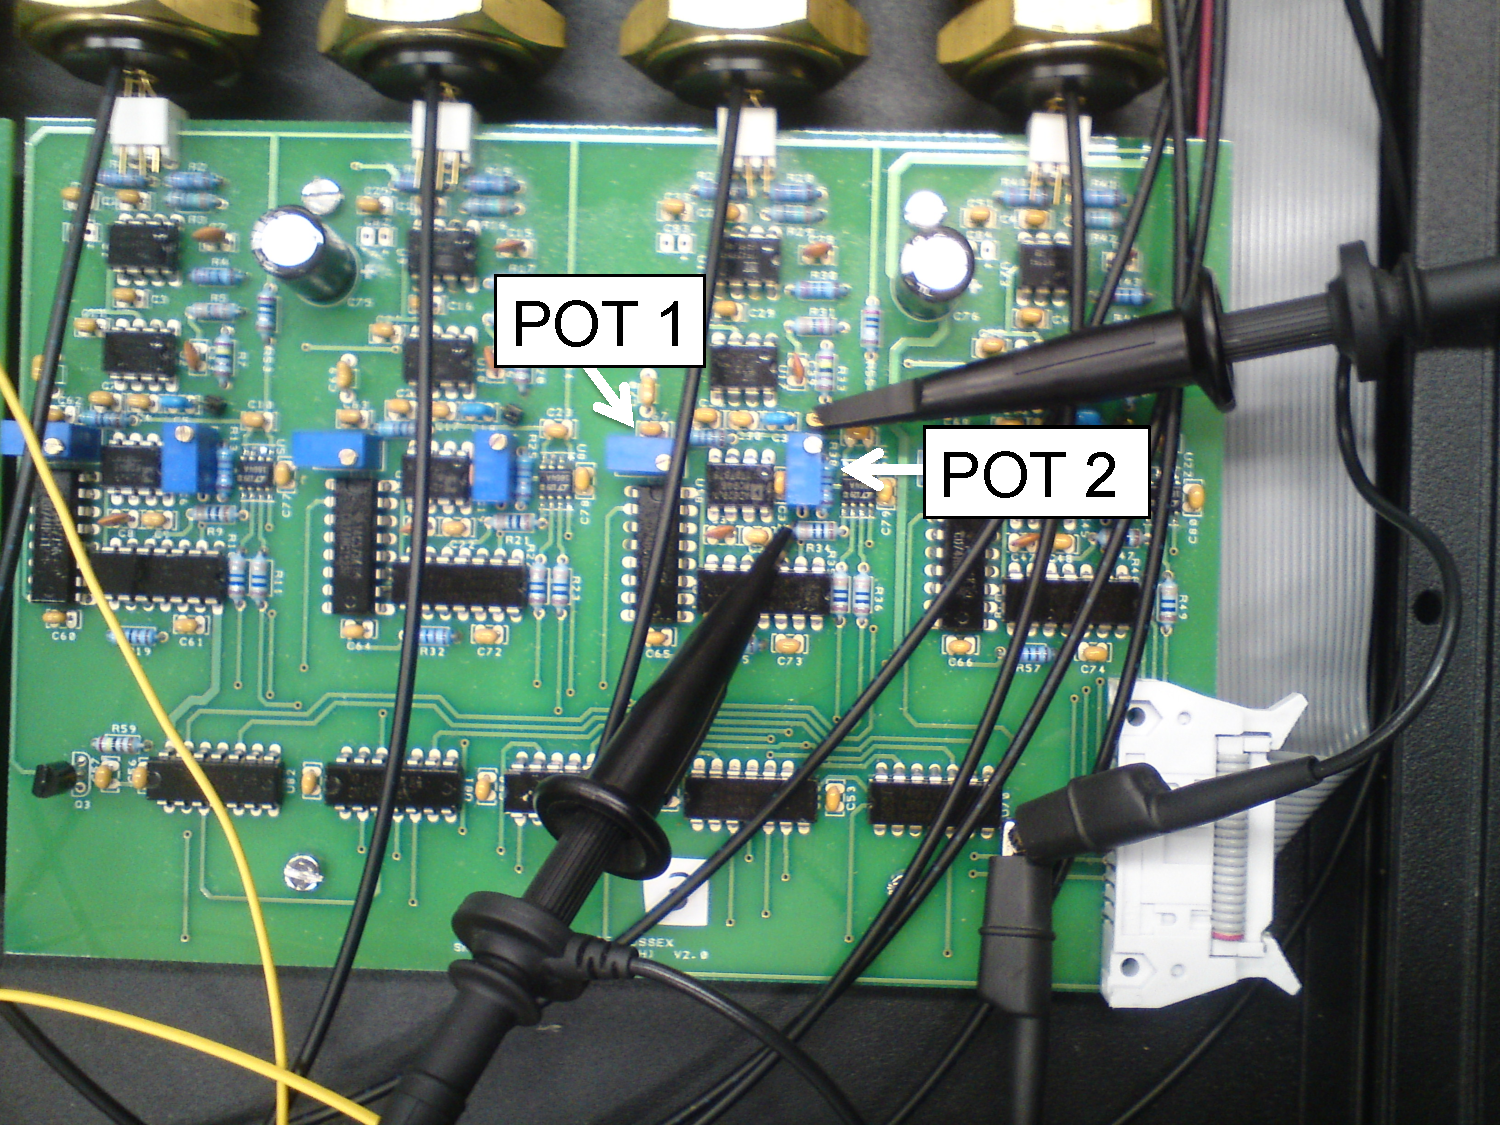
\includegraphics[width=0.50\textwidth]{PINPotentiometerPic}} 
	\subfloat[Scope displaying PIN pulse (CH1) and sample point (CH2), the gain determines the aptitude of the pulse.]{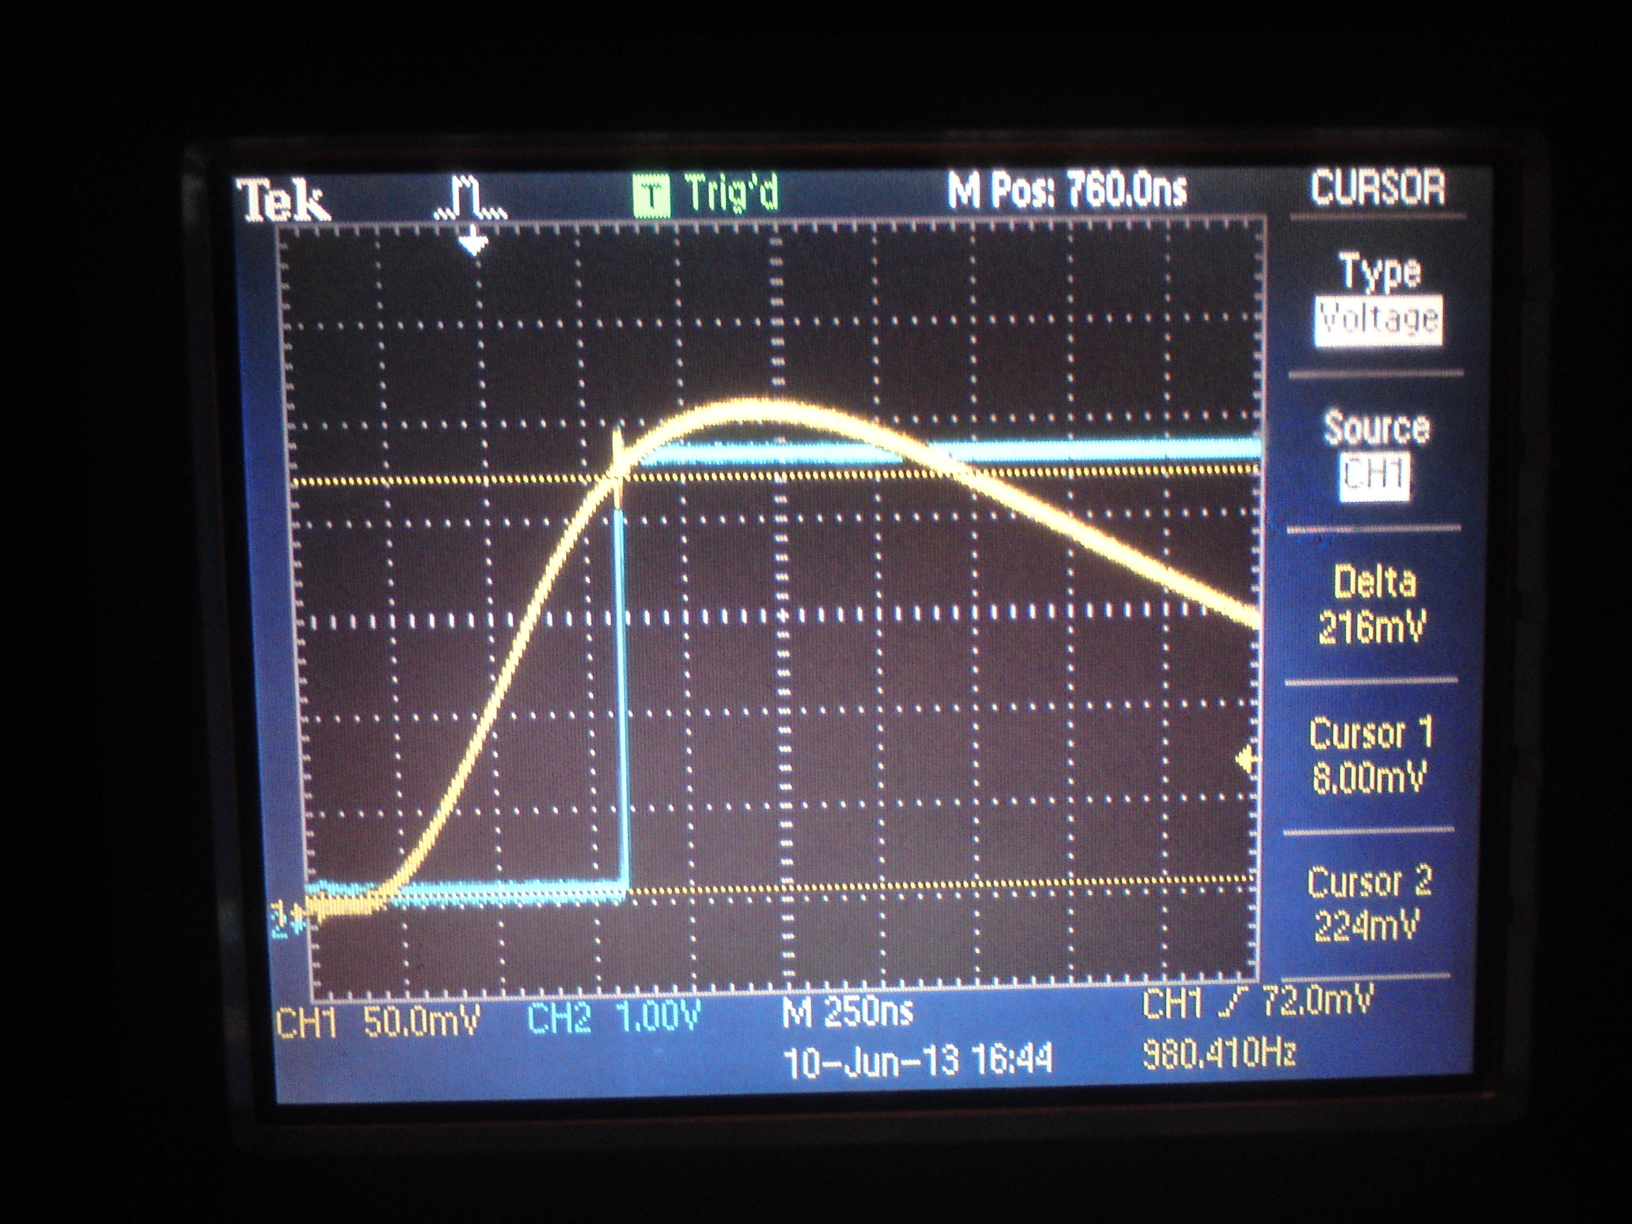
\includegraphics[width=0.50\textwidth]{PINSignalPickOff}}
	\caption{PIN diode probes and pulse shape.}
	\label{fig:PINDiodePots} 
\end{figure}


\subsection{Board designs \& description}
\label{subsec:PINDesigns}
This section is currently just a place holder. The included schematic is a little out of date. Richard White at Sussex is working on a full write up for this section. 

\begin{figure}[htbp]
	\begin{center}
		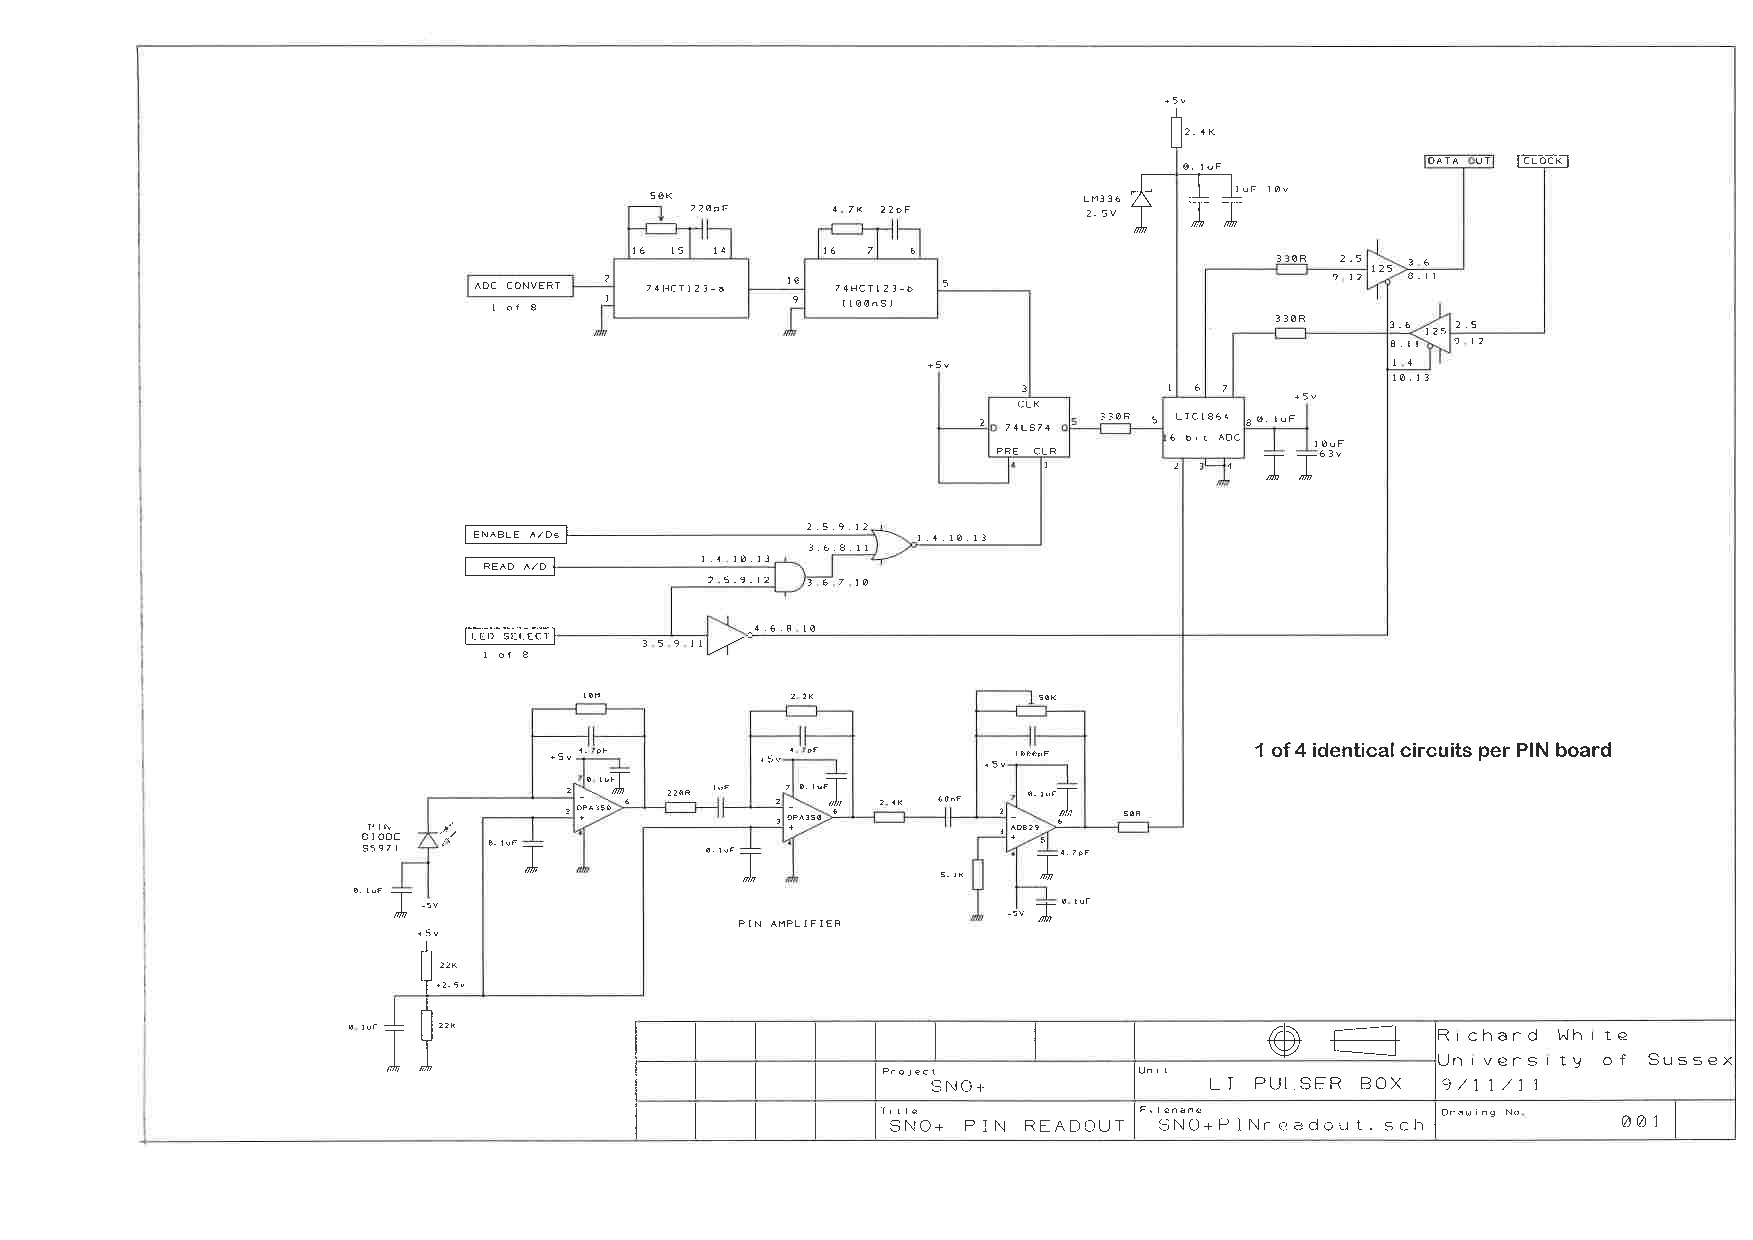
\includegraphics[width=1.0\textwidth]{PINSchematicDesign}
		\caption{Schematic design of the PIN diode circuit.}
		\label{fig:PINSchematicDesign}
	\end{center}
\end{figure}



\subsection{Performance}
The bulk of TELLIE's operation will be in the 10$^3$ photons per pulse regime. During channel-to-channel calibrations at site in 2015 the PIN diodes response was optimised for operation in this low intensity region. As a result the PIN's response saturate at high light outputs, typically at outputs \textgreater 50,000 photons per pulse. 

\chapter{In-situ hardware}
\label{chap:inSitu}
The `in-situ' hardware is an umbrella term for any of the TELLIE hardware which is inside the SNO+ cavity. This includes: One hundred and ten, 45~m duplex PMMA optical fibres which guide the light from the patch pannel on the electronics deck to the fastening points on the PSUP (92 fibres for installing + 18 spares) \cite{tellieFibreHardware}, the feed-through-assembly which provides a light-tight seal for passing the optical fibres from the deck into the cavity \cite{feedThroughDrawings}, and the mounting plates which the fibres couple into, mounted on the PSUP nodes \cite{telliePlatesDrawings} \cite{amelliePlatesDrawings}. A full, in detail, description of TELLIE's in-situ hardware is given in \cite{tellieFibreHardware}. Some further details, including installation procedures for all of the ELLIE systems are given in \cite{ellieInstall}. To avoid redundancy, that information will not be repeated here, we will, however, briefly summarise the logic associated with the in-situ hardware. 

The design of the placement and mechanical structure of the TELLIE fibres system is determined by the requirement of providing a coverage of the PMTs as uniform as possible, and by the access constraints to the existing detector structure. 

The $\sim$9500 PMTs are mounted with light reflectors within hexagonal-shaped boxes called``hex cells'', made of Acrylonitrile Butadine Styrene (ABS), see Figure~\ref{fig:HexCell}. These are assembled in flat pannels, supported by the PSUP. Most PMTs are mounted in triangular panels that follow the faces of the geodesic shape, these can be seen as triangular segments in Figure~\ref{fig:NodePanelMap}. However, close to each node, there is a much smaller panel of hexagonal shape, positioned where the node number labels are in Figure~\ref{fig:NodePanelMap}. These hexagonal distributions close to the nodes were chosen to host the ELLIE mounting plates, since they have a slightly wider gap with respect to the neighbouring panels, facilitating installation. These locations are also convenient in that their distribution in the detector guarantees in a simple way a uniform coverage of all the PMTs, when all 91 nodes and the neck aperture are used. A flat map of the PSUP structure with each of the 91 nodes labelled is given in Figure~\ref{fig:NodePanelMap}. The same map is shown with each of the 95 installed TELLIE channels labelled is given in Figure~\ref{fig:NodeChannelMap}.

The number of LED-driver channels is 96, chosen to be slightly larger than the required 92 in order to ensure some redundancy in case of channel failure. The number of fibres installed is also higher, 110 double cables, in order to have enough spares in case of breakage during installation.

\begin{figure}[htp]
	\begin{center}
		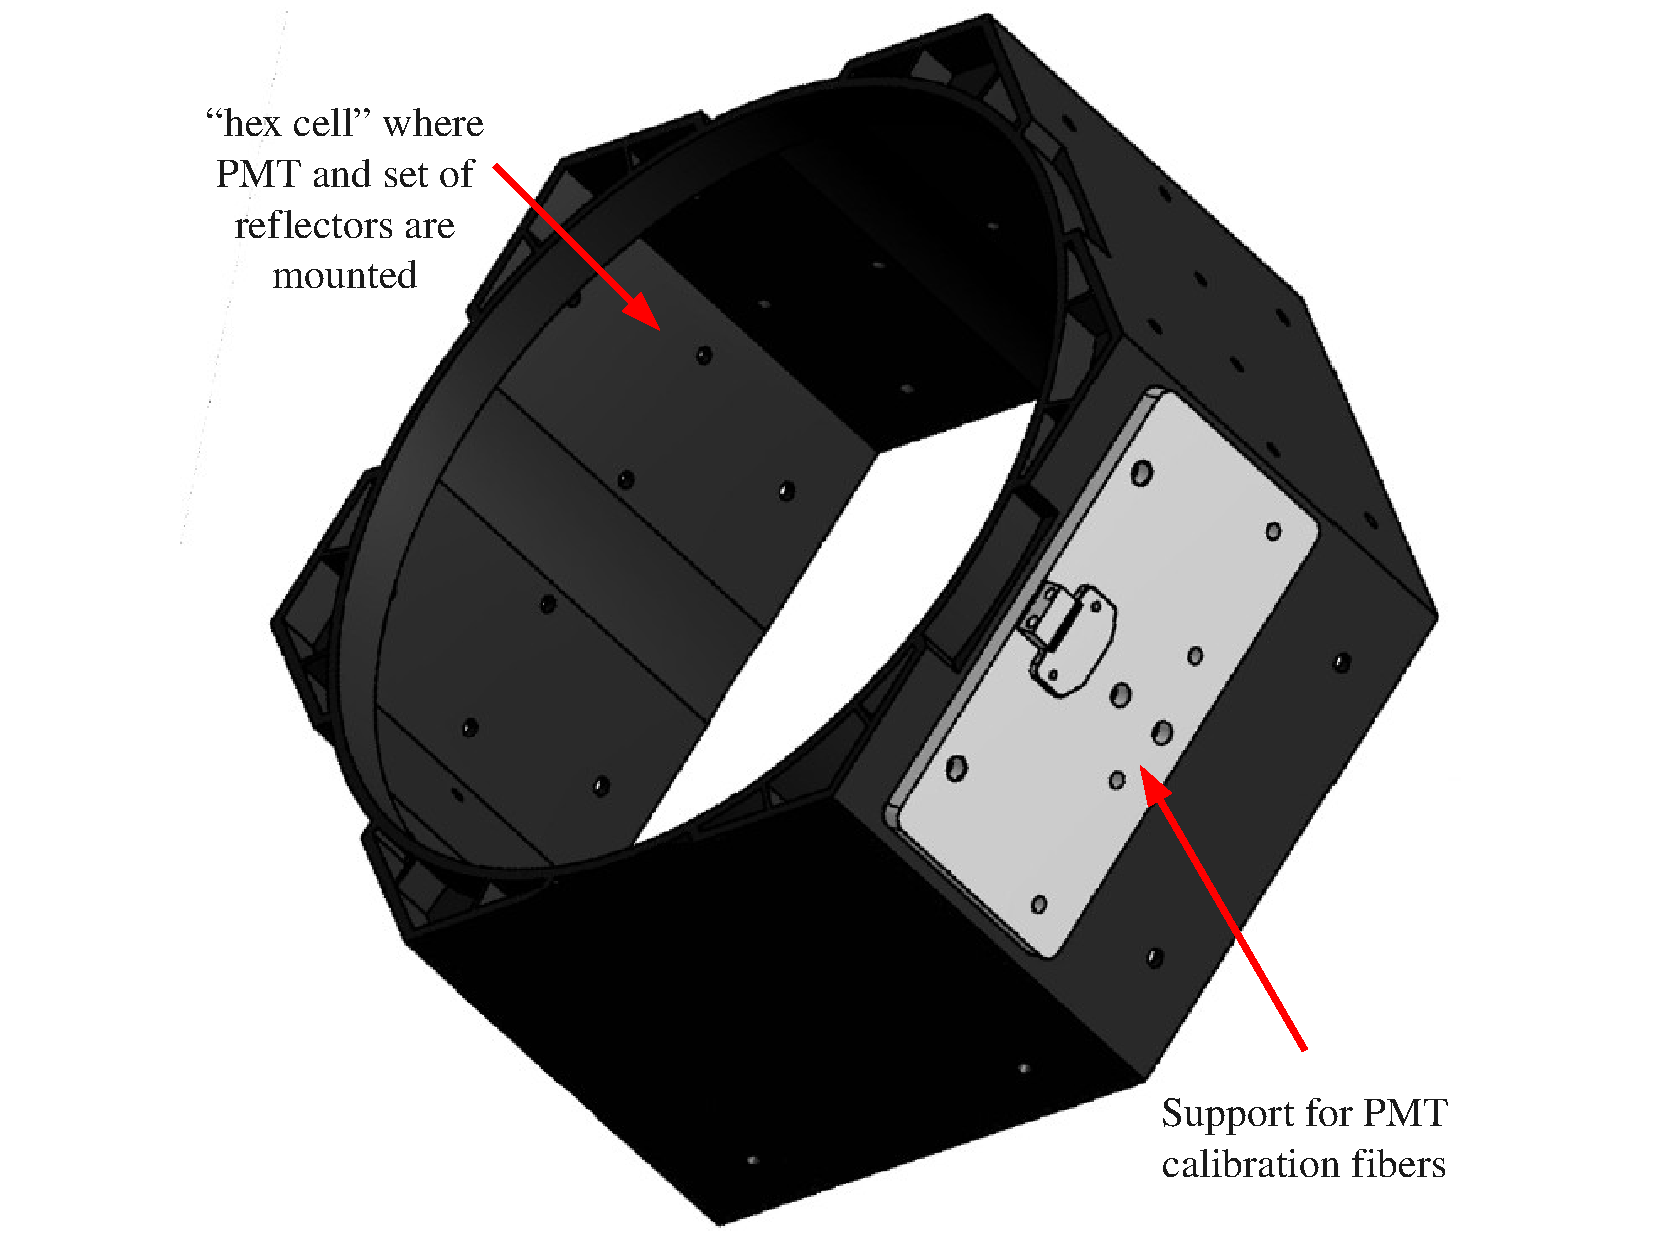
\includegraphics[width=0.5\textwidth]{HexCell}
		\caption{Illustration of a SNO+ PMT casing (hex cell) with a mount fitted for TELLIE fibres. The hex cell is approximately 30~cm across.}
		\label{fig:HexCell}
	\end{center}
\end{figure}

\begin{figure}[htp]
	\begin{center}
		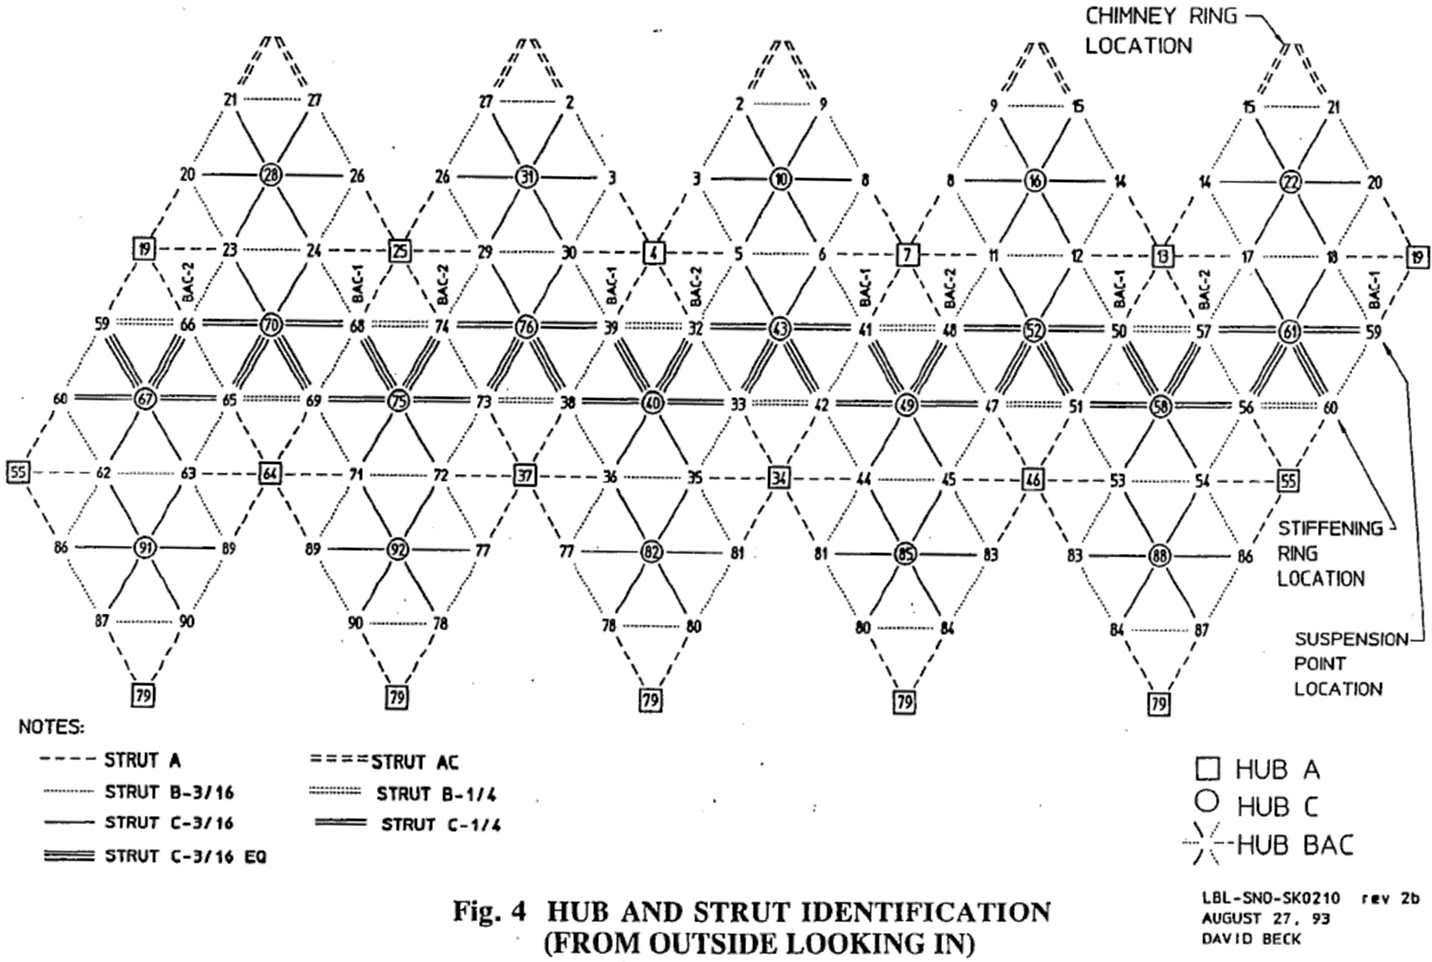
\includegraphics[width=0.9\textwidth]{NodePanelMap}
		\caption{Schematic of the SNO+ PSUP structure. A TELLIE duplex fibre is installed at each node.}
		\label{fig:NodePanelMap}
	\end{center}
\end{figure}

\begin{figure}[htp]
	\begin{center}
		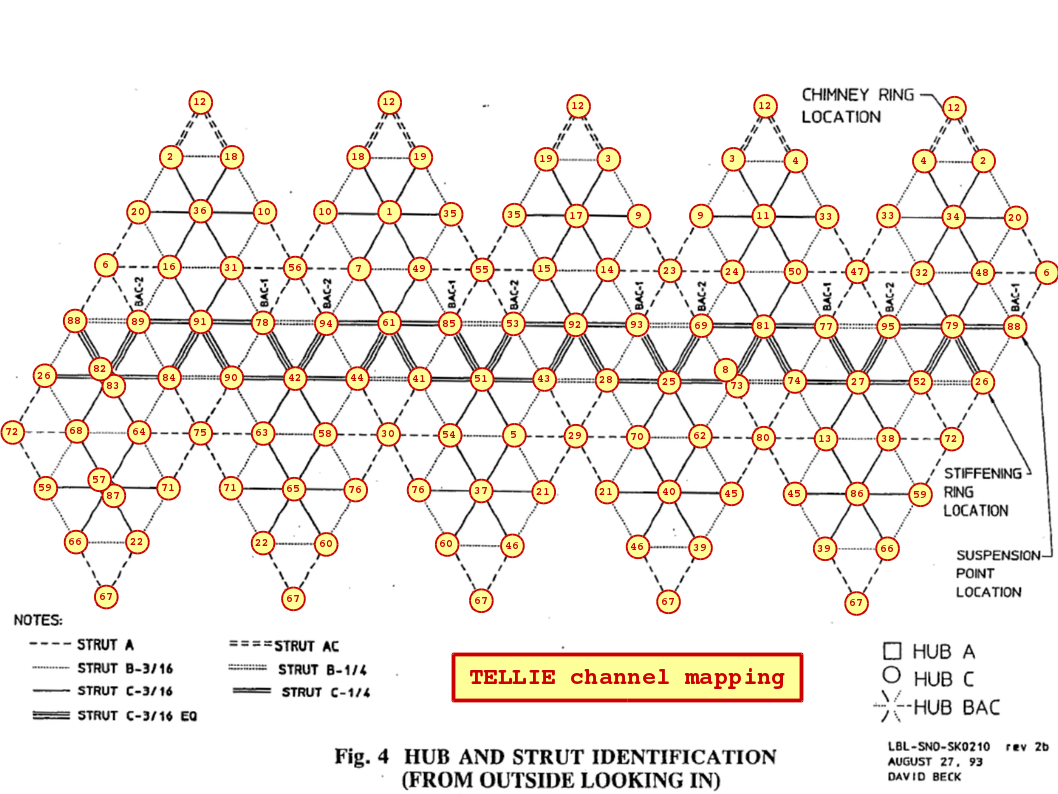
\includegraphics[width=0.9\textwidth]{NodeChannelMap}
		\caption{Schematic of the SNO+ PSUP structure, numbering TELLIE channels instead of PSUP nodes. Three nodes have a second fibre installed for redundancy.}
		\label{fig:NodeChannelMap}
	\end{center}
\end{figure}

\chapter{Known quirks \& behaviours}
\label{chap:Quirks}
This section is intended as a reference for future users of the TELLIE system. In the long commissioning campaign, beginning at Sussex in 2013 and finishing at SNOlab in 2016, a number of unexpected and unexplained behaviours have been observed. These behaviours are detailed in the sections which follow in this chapter. 

\section{PIN diode effects: Observed at Sussex July 2016}
A number of effects in the PIN diodes response have been observed during a testing period at Sussex in August 2016. A number of PIN diode boards had been identified as poorly performing during a period of recalibration at site by Mark S. The typical definition for a poorly performing channel is a noise level significantly above well performing channels on at least one of the four channels. There is not a quantitative measure for what defined a poorly performing board. Essentially they've just been `eyeballed'.

This section describes the test proceedure and the results of that testing regime. It should be noted that, despite being flagged as poorly performing (to different degrees) at site, all 8 boards brought back and tested behaved quantitatively very consistently. The rest of this section describes some of the notable observations from this testing regime. Only example plots are given in this section, to see the plots for all boards tested, please see \cite{telliePINeffects}. 

In master mode the pulse delay was set to 1~ms, in slave mode a TTL signal generator was used to trigger TELLIE at 1~kHz. All PIN diode boards tested (8 in total) were driven by the same LED driver boards, serial numbers: 100, 99, 10, 9. These four driver boards are permanently installed in the Sussex test box. All data was taken by addressing the Sussex text box as Box 1 and simply replacing the PIN readout board. Sussex test box is powered by a linear mode desktop supply on the +5V line. The -5V and -7V lines are supplied though switch mode supplies identical to those used at site, the AC for which is supplied via a 110V transformer. IPW sweeps were run from high IPW to low IPW. We have observed in the past that running at low IPW first (i.e. max light output) seems to settle both the driver and the PIN diode response. Sweeps were therefore run in reverse to avoid artificially reducing the apparent noise on the system’s response. All uncertainties shown on the plots which follow are the error on the mean (i.e. RMS / sqrt(noPulses)).

\subsection{Flat PIN response}
In the case the system is turned on from cold it was observed that at least one of the four channels on a PIN readout board would return a flat PIN response over the full operational range. This effect would be repeated if the sweep was simply re-run. 

\textbf{This effect was resolved in 100\% of cases if a 1000 pulse sequence was requested before the sweep at a light level above zero (typically at IPW $\sim$ 7000)}. 

\begin{figure}[htp]
	\begin{center}
		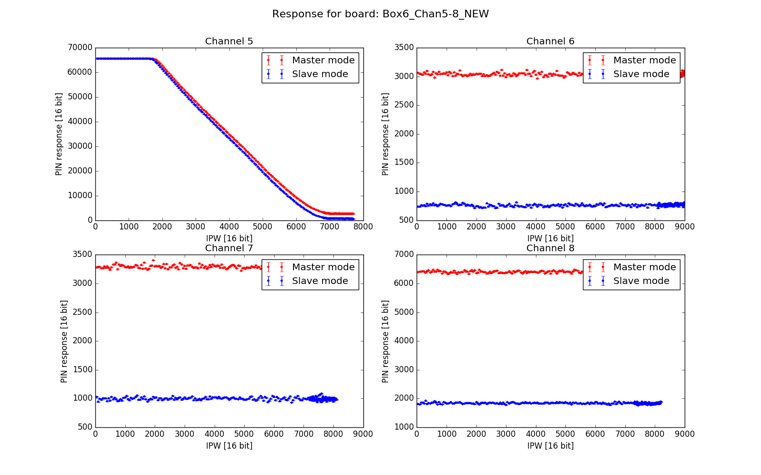
\includegraphics[width=0.8\textwidth]{PINFlatResponse}
		\caption{An example of the described `flat response' when a sweep was run on a board just after switching the system on.}
		\label{fig:PINFlatResponse}
	\end{center}
\end{figure}

\subsection{Master / Slave mode PIN response discrepancy}
It has been observed that an offset exists between the PIN diodes response when operating in master / slave mode. The absolute offset varies between channels, but the four channels presented in Figure~\ref{fig:PINDiscrepancy} are typical.

\begin{figure}[htp]
	\centering
	\subfloat[Full operational range]{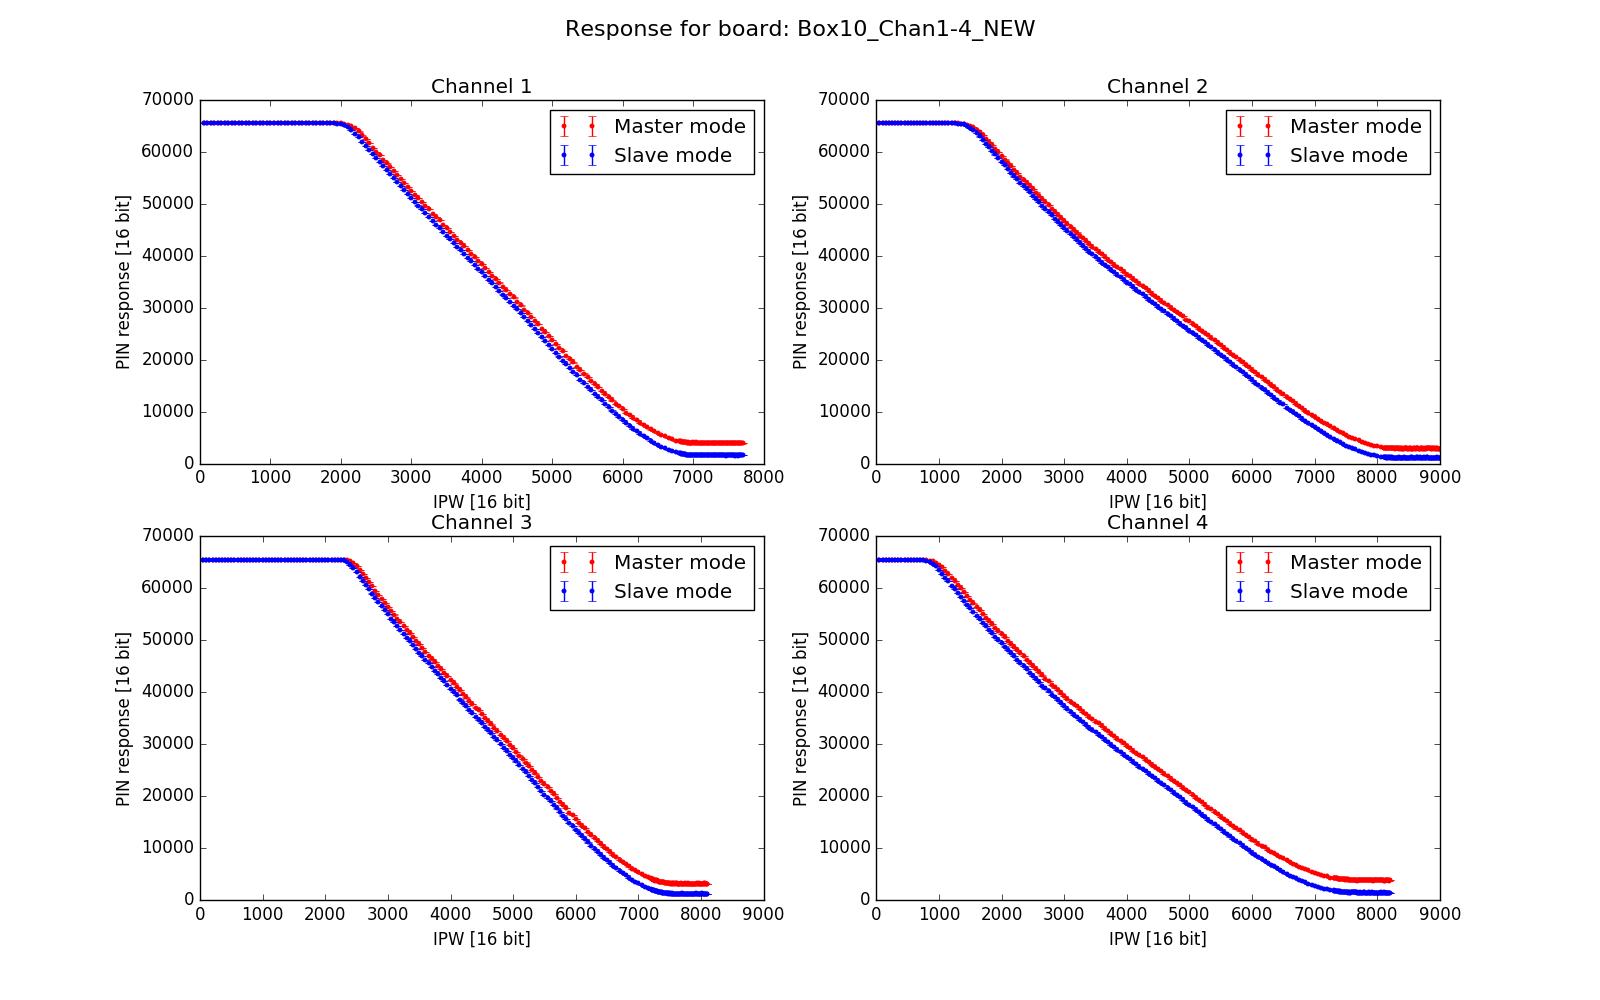
\includegraphics[width=0.50\textwidth]{PINDiscrepancyFull}} 
	\subfloat[Low intensity range]{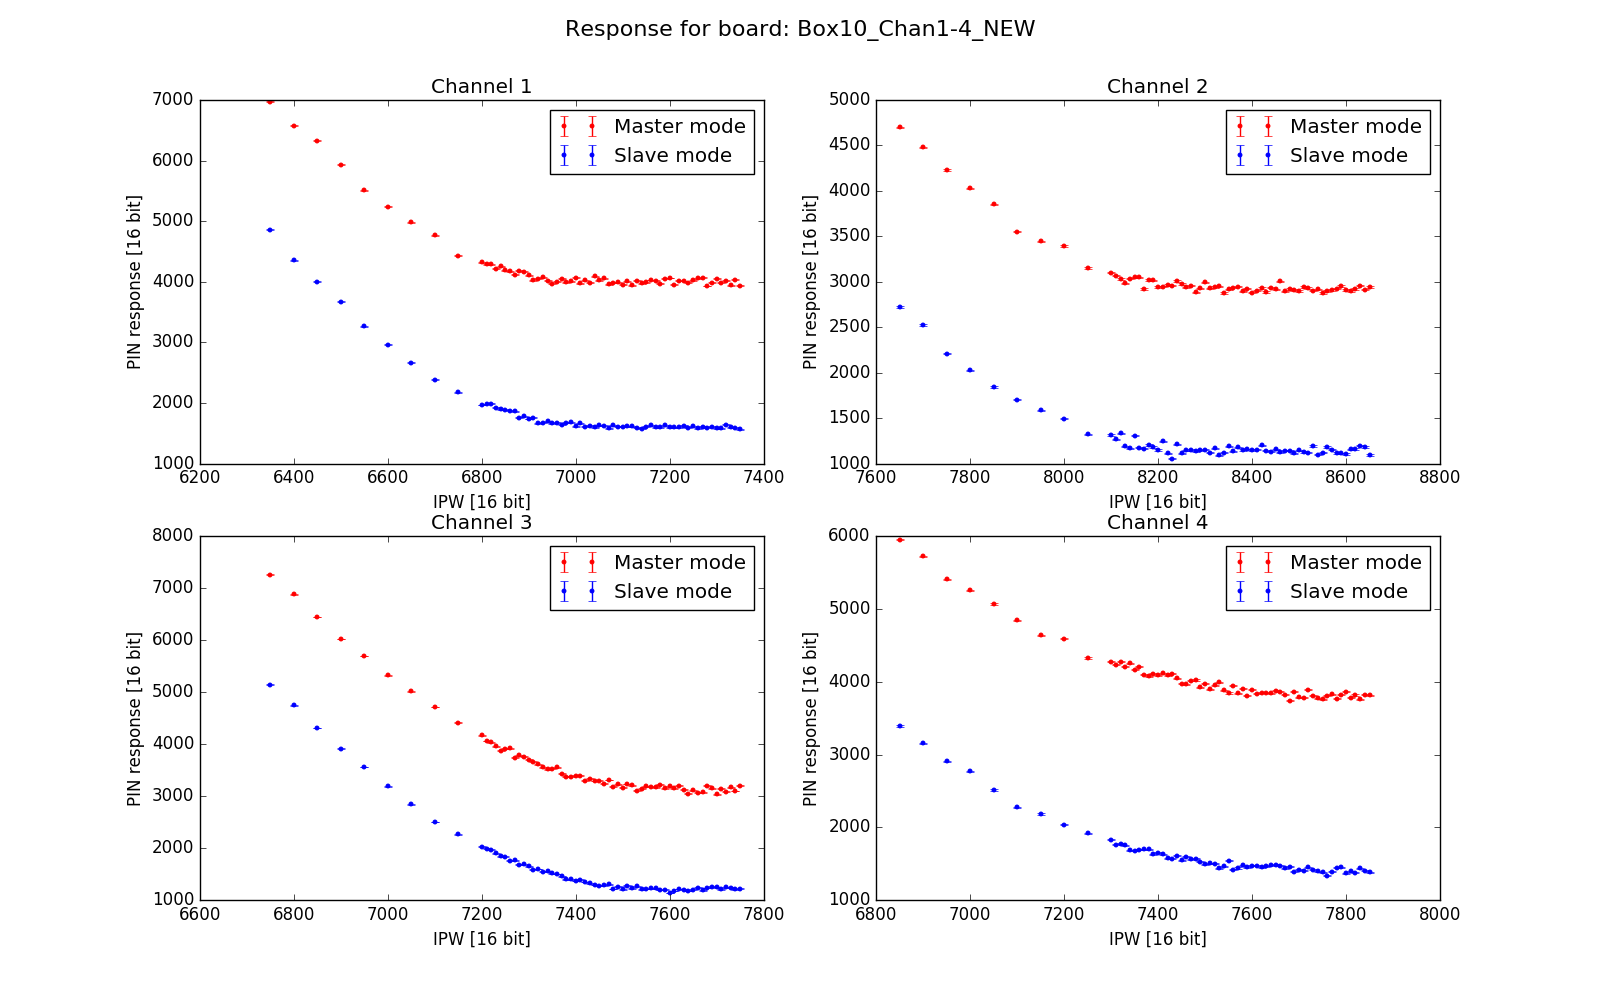
\includegraphics[width=0.50\textwidth]{PINDiscrepancyLow}}
	\caption{PIN measurements taken as a function of IPW setting for all four channels associated with a single read out channel. An offset is observed in the response when running in master and slave modes.}
	\label{fig:PINDiscrepancy} 
\end{figure}

\subsection{Slave mode `Dip'}
A dip in the PIN diode response was observed on two instances when operating in slave mode: Box 6 Channel 8 \& Sussex test board Channel 8. In both cases the sweep was re-run three times. The same behavior was observed each time.

\begin{figure}[htp]
	\centering
	\subfloat[Box 6, Channel 8]{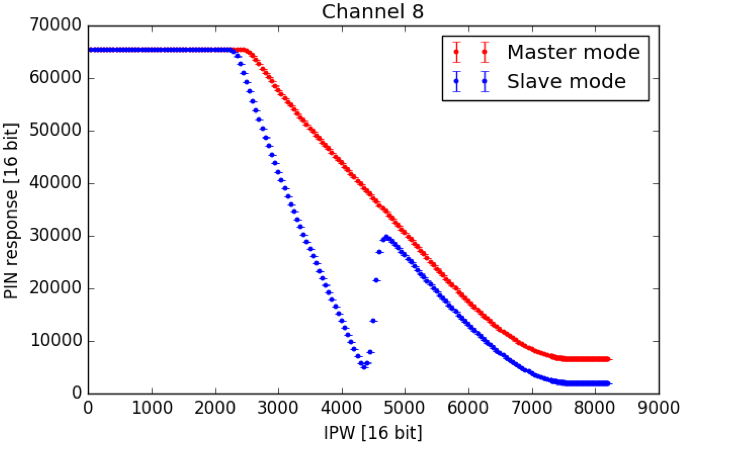
\includegraphics[width=0.50\textwidth]{PINDip1}} 
	\subfloat[Sussex test board]{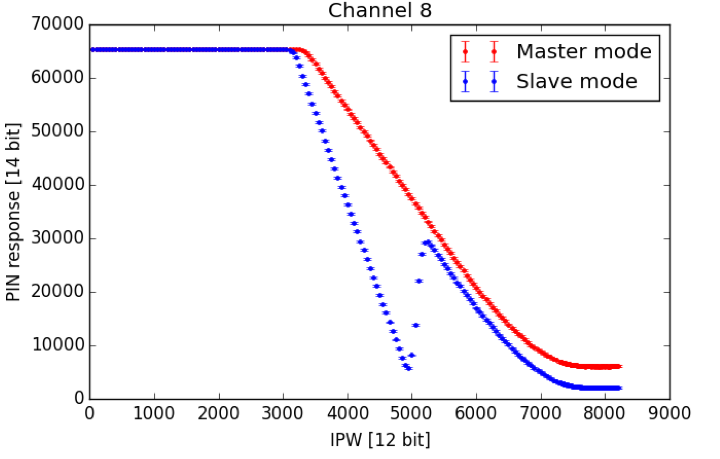
\includegraphics[width=0.50\textwidth]{PINDip2}}
	\caption{The dip observed in the slave mode PIN diode response of two of the 32 channels checked.}
	\label{fig:PINDip} 
\end{figure}

\subsection{Upper / Lower addressing discrepancy in RMS}
As described at the beginning of this section, all Sussex test bench measurements presented in this section simply replaced PIN readout boards in a box addressed as box 1. In a test (outside of the scope of the rest of the data presented here) it has been observed that the rms measured when using the same hardware, but simply attaching the ribbon cable to the control box’s upper port, changes significantly.

\begin{table}[t]
	\centering
	\begin{tabular}{| c | c | c | c |}
		\hline                        
		& Slave mode & Master Mode \\ \hline \hline
		Box 1 (channel 8) & \textbf{2170} $\pm$ \textbf{172.9}  & 5937 $\pm$ 181.4 \\ \hline
		Box 8 (channel 8) & \textbf{2210} $\pm$ \textbf{6.16}   & 6125 $\pm$ 179.7 \\ \hline
	\end{tabular}
	\caption{Showing the reduction in rms observed when taking an RMS reading from the upper set of boxes when operating in slave mode.}
	\label{tab:PinAdressing} 
\end{table}

\section{Underground effects}
In the summer of 2015 a full calibration of the channel-to-channel of TELLIE's response was run in the underground environment. To do so, the whole system was removed from the ELLIE rack and temporarily set-up on a bench in the SNO+ control room. The power box was connected into a standard 110~V mains power socket at the back of the room. Detailed procedures for this calibration can be found at \cite{tellieCalibProceedures}. During this time we identified a number of LED driver and PIN diode boards which performed poorly relative to the rest of the system were identified \cite{aug2015CalibSummary}. 

In January 2016 a number of replacement board were brought to site, to be installed and calibrated by Mark S. Before the boards were replaced the TELLIE system was again removed from the SNO+ control rack and set-up again in the SNO+ control room. The identified boards were re-tested and showed notably different results. A full description of all of the work done underground by Mark can be found at on his blog page which he used to produce TELLIE-specific shift reports \cite{StringerBlog}. This observation of the inconsistent response of individual channels lead to Mark undertaking a significant campaign of underground testing, including a second full calibration of all channels (a number of which had hardware replaced). A number of the observations from that campaign are described here.

\subsection{PIN diode warm up effects}
When running a low intensity sweep (as part of the calibration procedures given in \cite{tellieCalibProceedures}) a specific `s' shaped pattern was observed in the Photon Vs PIN reading correlations. This effect was rare and difficult to re-produce, but seemed to be correlated to the system recently being switched off. In that sense it is similar to the `flat' response observed at Sussex - although (perhaps because the sweep always run from high intensity to low intensity in the calibrations) the flat response has never been observed underground. An example of this s-shaped warm up is given in Figure~\ref{fig:PINWarmUp}.

\textbf{This effect always disappeared when the low intensity sweep was re-run.}

\begin{figure}[htp]
	\begin{center}
		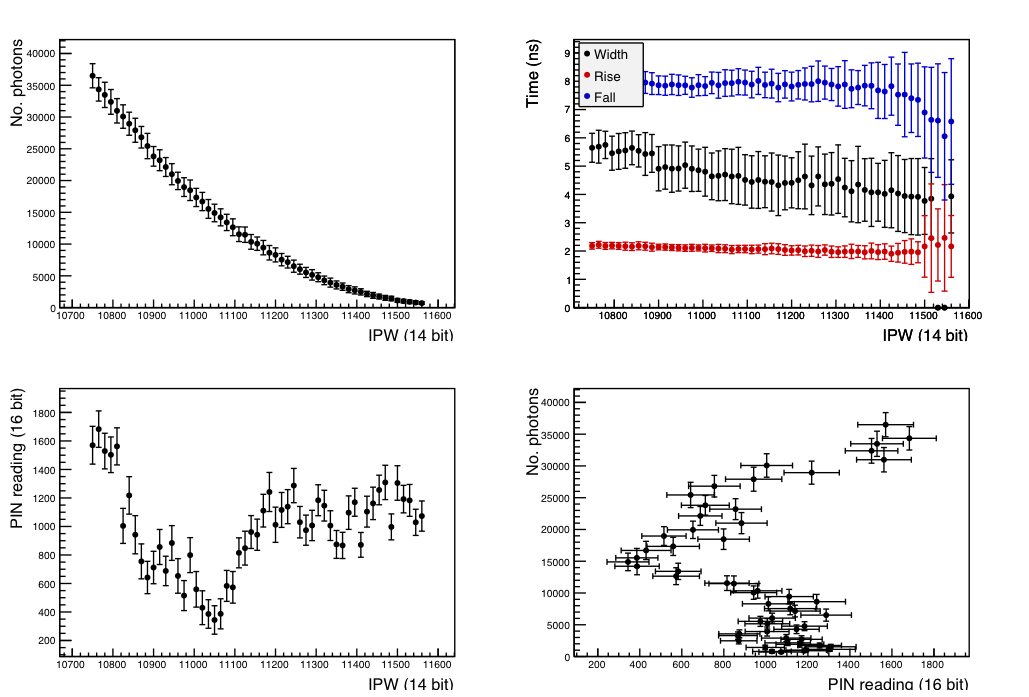
\includegraphics[width=0.8\textwidth]{PINWarmUp}
		\caption{An example of PIN diode warm up effect. This plot was taken using channel 32 during re-calibrations in Spring 2016}
		\label{fig:PINWarmUp}
	\end{center}
\end{figure}

\subsection{PIN diode response quantisation}
As part of a test to probe the correlations between TELLIE response and external stimuli (for example probing the voltage on one of the power lines - tried at a number of points in the system), a single TELLIE channel was continuously pulsed in sequence mode. Measurements of the photon output and PIN response were measured using the same methods as when acquiring calibration data, i.e. a calibrated PMT read out by an oscilloscope. 

Through running this data acquisition script it was observed that, even when the system was not interfered with directly, jumps would be seeing the the PIN diodes response. These jumps could be caused on demand by simply touching the tellie box casings. The speculation is that this is due to grounding issues. Examples of this effect happening both with and without external stimulus are given in Figure~\ref{fig:PINQuantisation}. Both measurements were taken on Channel 18 in May 2016. 

\begin{figure}[htp]
	\centering
	\subfloat[An observation without human interaction]{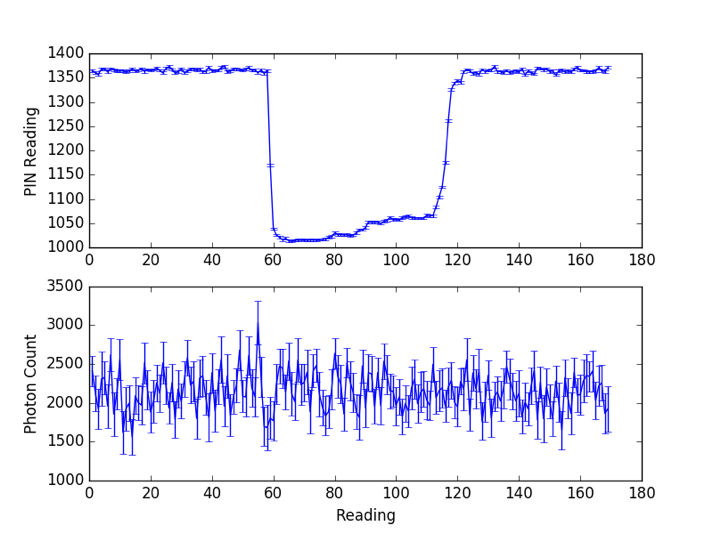
\includegraphics[width=0.50\textwidth]{PINQuantisation1}} 
	\subfloat[An observation with human interaction]{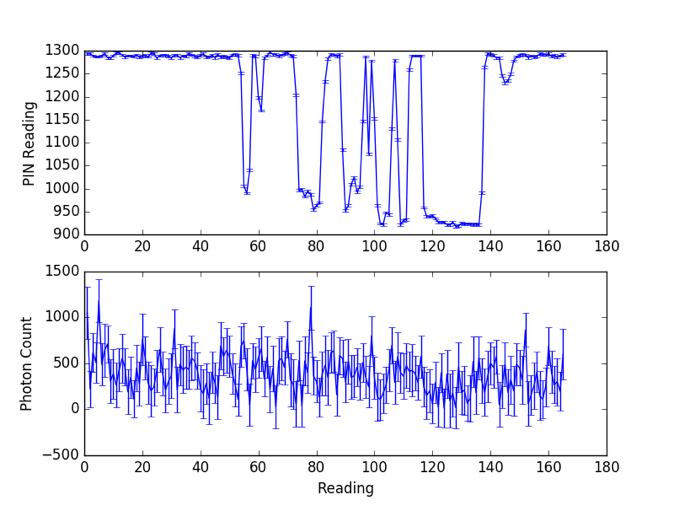
\includegraphics[width=0.50\textwidth]{PINQuantisation2}}
	\caption{Plots showing trends towards a two level quantisation in the PIN diodes response. (a) Shows a data set taken over a coffee break. The system was subject to no known external stimulus. (b) Changes in response created by touching the active TELLIE driver box. When the box was touched with a bare hand the PIN response reduced. The photon output throughout the test (as measured by the calibrated PMT) is plotted in the lower subplot. In both cases it is observed to be constant.}
	\label{fig:PINQuantisation} 
\end{figure}

\subsection{LED driver warm up effects}
During a campaign of testing in early 2016 a warm up effect was noticed when running low intensity sweeps on individual channels. The cause is unknown, but likely due to some capacitive charging in the circuit. The effect is observed most prominently when the system had recently been powered back up. 

\begin{figure}[htp]
	\centering
	\subfloat[]{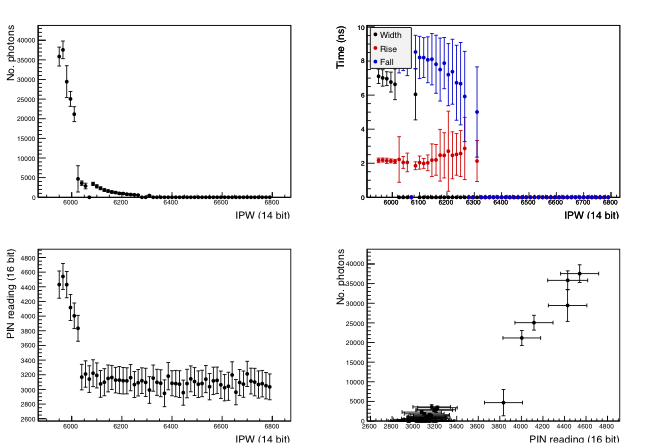
\includegraphics[width=0.50\textwidth]{DriverWarmUp1}} 
	\subfloat[]{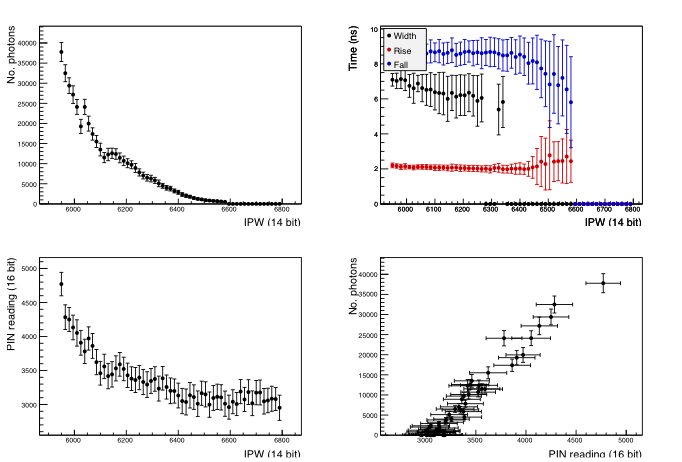
\includegraphics[width=0.50\textwidth]{DriverWarmUp2}}
	\newline
	\subfloat[]{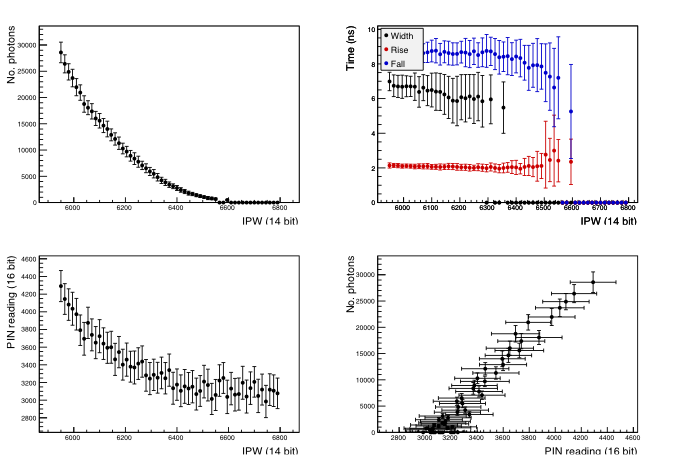
\includegraphics[width=0.50\textwidth]{DriverWarmUp3}}
	\caption{Three consecutive low sweep measurements taken on channel 73. A warm up effect is observed and the photon output settles to the expected shape. A smaller effect is also observed in the PIN diode response.}
	\label{fig:DriverWarmUp} 
\end{figure}

\subsection{Slave mode trigger out}
It has been noticed during the Slave mode calibrations run by Mark S in 2016 that \textbf{a trigger will not be produced if the system is run in slave mode after a power cycle. This can be solved by running a short burst of pulses in master mode}. The cause is unknown, but the solution is simple. It is possible for a short bust of master mode pulses could be built into standard runs through ORCA, although, at the time of writing (Oct. 2016) that is not implemented. 

\section{Calibration drift}
Due to a specific incident during May 2016 dark running, where TELLIE's photon output was orders of magnitude higher than requested, some studies were run to investigate any drifts in the calibrated response of individual TELLIE driver channels. This section summarises those studies. Slides outlining the specifics of the issue itself, including attempts to debug it, are given in \cite{tellieInsensityIssue}. 

\subsection{Method and considerations}
At the time of this study two full calibrations of the channel-to-channel response of TELLIE had been performed; one done at Sussex in Summer 2013, and one at site in the Summer of 2015. In both cases a calibrated benchtop PMT was used to measure the light output of each channel as a function of IPW. As a result, both photon output calibrations are dependent on the calibration of the benchtop PMTs used in each case. In an attempt to decouple this dependence and convince ourselves that the accuracy of the PMTs calibration was, in both cases, reasonable we first compare each calibration to set points used for PCA data taken in December 2014. The channels and set points used during this campaign of data taking can be found at \cite{tellieDataDec2014}. 

In this case the IPW set point of each channel was tuned independently of the calibrations to give $\sim$75 nHits with the detector partially filled with water. We assume a nHit of $\sim$75 nHit is equivalent to a photon output of 1000 photons / pulse \cite{tellieHitProbablities}. By subtracting the set point used to produce $\sim$75 nHit in PCA data from the calibration 1000 photon / pulse set point a comparison can be made between between calibrated set points and the detector system's response.  


\subsection{Comparison to December 2014 dark running set-points}
\label{subsec:calibVsData}
There is a major difference between the 2013 and 2015 calibrations data sets. The 2013 calibration taken at Sussex only provides three set points: 1e3, 1e4 and 1e5 photon / pulse set points. The 2015 calibration acquired much more finely grained data in the same range before applying a parabolic fit. The parameters of this fit are used to calculate the required IPW set point for a requested photon output. 

The set points used to acquire 2014 PCA data were then subtracted from the equivalent 1e3 photon/pulse set points given by the 2013 \& 2015 calibrations on a channel-by-channel basis, results can be seen in Figure~\ref{fig:CalibMinusData}. 

\begin{figure}[htp]
	\centering
	\subfloat[2013 Calibration]{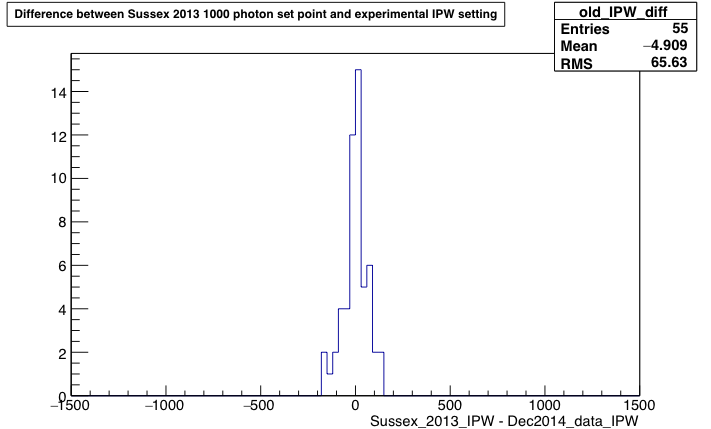
\includegraphics[width=0.50\textwidth]{CalibMinusData2013}} 
	\subfloat[2015 Calibration]{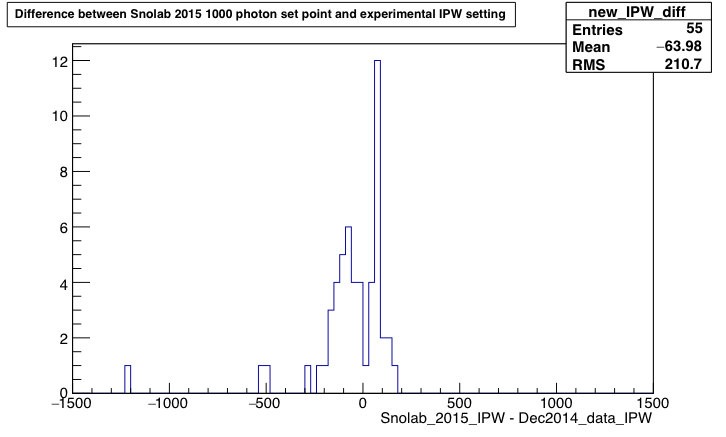
\includegraphics[width=0.50\textwidth]{CalibMinusData2015}}
	\newline
	\subfloat[2015 Calibration - interpolated]{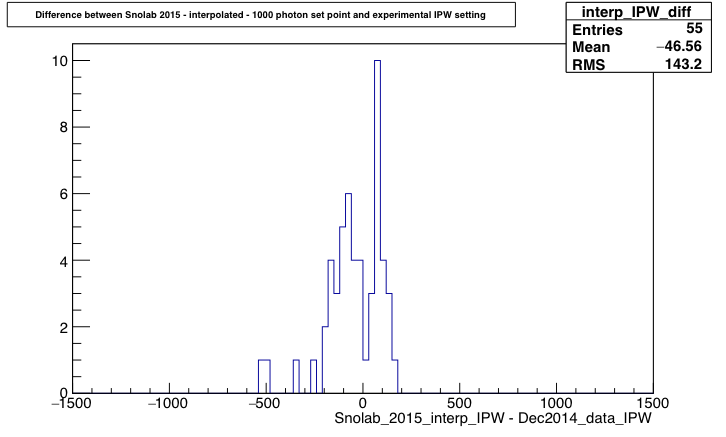
\includegraphics[width=0.50\textwidth]{CalibMinusDataInterp}}
	\caption{Plots showing the difference between the calibrated setpoints and PCA setpoints used to produce $\sim$75~nHit in air fill.}
	\label{fig:CalibMinusData} 
\end{figure}

The key feature in these plots is that they sit about 0. This result gives us confidence that the desktop PMT's calibration was consistent in both cases. An additional, notable feature is observed in Figure~\ref{fig:CalibMinusData}b, where a splitting or `double peak' is seen about the 0 point. To check this isn't a systematic effect associated with the fit method used in this calibration a second method was applied to the calibration data extract a set point. In this second case, rather than fitting the data, we applied and interpolation method on the calibrated curve. That is, we find the points bounding the 1000 photon / pulse intensity point draw a straight line between them and use the line's equation to calculate the associated IPW set point. The results using this interpolation method are shown in Figure~\ref{fig:CalibMinusData}c. No significant differences can be observed when comparing the two techniques (Figures b) and c)). It appears to be a real effect. 

\subsection{Direct calibration-to-calibration comparisons}
\label{subsec:calibToCalib}
With confidence that there is no major systematic offset between the 2013 and 2015 calibrations, the set points of each can be compared directly. Histograms showing the channel-by-channel subtraction of the at the 10$^3$, 10$^4$ and 10$^5$ photons/pulse set points are presented in Figure~\ref{fig:CalibToCalib}. Additionally the channel-to-channel set points have been plotted against each other in Figure~\ref{fig:CalibCorrelations}, where the fitted straight line gradients further quantify the offsets observable in Figure~\ref{fig:CalibToCalib}. 

It is observed that at higher photon outputs an offset or \textbf{systematic calibration drift} is observed. The drift only appears for photon outputs above 10$^3$ photons/pulse, the reason for this drift is unknown. 

\begin{figure}[]
	\centering
	\subfloat[10$^3$ photons/pulse]{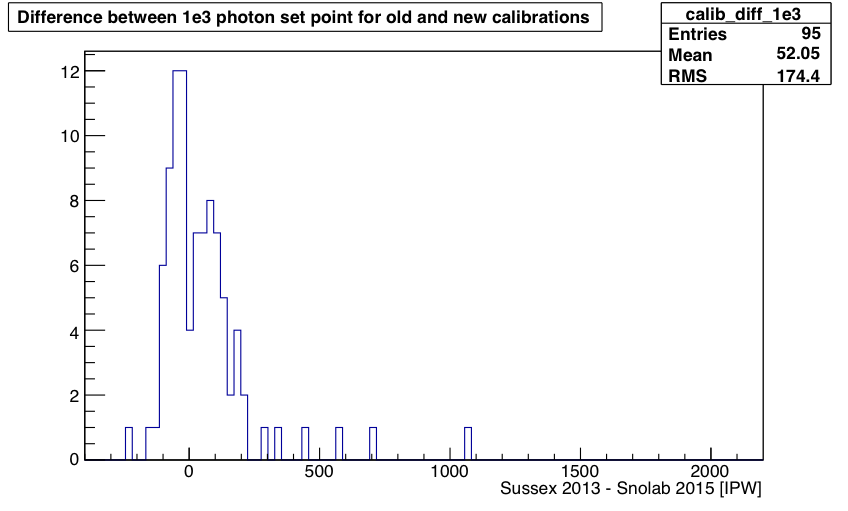
\includegraphics[width=0.50\textwidth]{CalibToCalib1e3}} 
	\subfloat[10$^4$ photons/pulse]{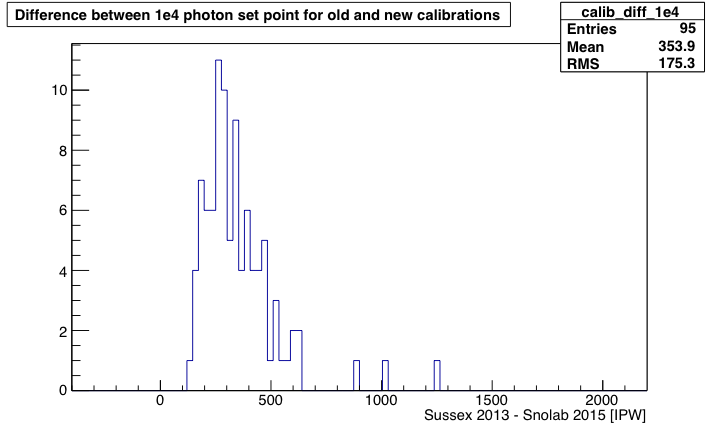
\includegraphics[width=0.50\textwidth]{CalibToCalib1e4}}
	\newline
	\subfloat[10$^5$ photons/pulse]{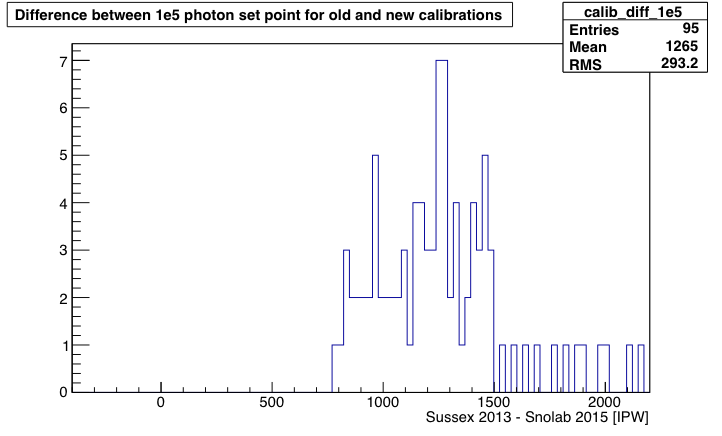
\includegraphics[width=0.50\textwidth]{CalibToCalib1e5}}
	\caption{Plots showing the difference between three intensity setpoints calibrated in 2013 \& 2015 }
	\label{fig:CalibToCalib} 
\end{figure}


\begin{figure}[]
	\centering
	\subfloat[10$^3$ photons/pulse]{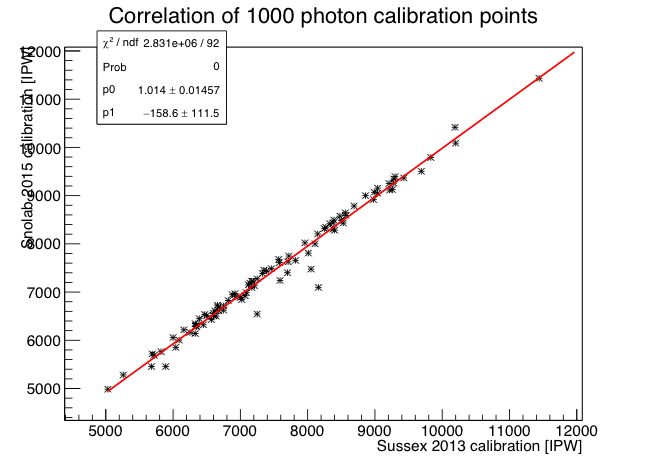
\includegraphics[width=0.50\textwidth]{CalibCorrelations1e3}} 
	\subfloat[10$^4$ photons/pulse]{\includegraphics[width=0.50\textwidth]{CalibCorrelations1e4}}
	\newline
	\subfloat[10$^5$ photons/pulse]{\includegraphics[width=0.50\textwidth]{CalibCorrelations1e5}}
	\caption{Correlations between calibrated set points. Straight line fits are used to quantify changes in gradient for each of the intensity settings.}
	\label{fig:CalibCorrelations} 
\end{figure}
 

%%%%%%%%%%%%%%%%%%%%%%%%%%%%%%%%%%%%%%%%%%%%%%%%%%%%%

\begin{thebibliography}{99}

	\bibitem[1]{elecSpecs} S.Peeters, ELLIE SMELLIE Specifications, DocDB-544, 2010.
	\bibitem[2]{PMTdescription} J. Boger et al., Nucl. Instr. and Meth. A 449 (2000) 172-207.	
	\bibitem[3]{snoTrigger} J.Klein et al, The SNO Trigger System, SNO-STR-97-035, 1997.
	\bibitem[4]{tubii} G.Orebi-Gann, TUBii \& CAEN, DocDB-1065, 2011.
	\bibitem[5]{RATtime} G. Orebi-Gann, Dealing with time in RAT, DocDB-481, 2010.
	\bibitem[6]{picManual} \url{http://ww1.microchip.com/downloads/en/DeviceDoc/39564c.pdf}
	\bibitem[7]{Sinclair} J. Sinclair, PhD Thesis, 2015.
	\bibitem[8]{tellieCode} TELLIE control code repo \url{https://github.com/snoplus/tellie}
	\bibitem[9]{NetworkManual} SNO+ network manual \url{https://www.snolab.ca/snoplus/private/DocDB/cgi/ShowDocument?docid=3122}
	\bibitem[10]{tellieFibreHardware} Description of TELLIE fibre hardware \url{https://www.snolab.ca/snoplus/private/DocDB/cgi/ShowDocument?docid=501}
	\bibitem[11]{ellieInstall} ELLIE install procedures \url{https://www.snolab.ca/snoplus/private/DocDB/cgi/ShowDocument?docid=2778}
	\bibitem[12]{telliePlatesDrawings} TELLIE mounting plate technical drawings \url{https://www.snolab.ca/snoplus/TWiki/bin/view/Main/DwgEng73}
	\bibitem[13]{feedThroughDrawings} TELLIE feed through box technical drawings \url{https://www.snolab.ca/snoplus/TWiki/bin/view/Main/DwgEng74}
	\bibitem[14]{amelliePlatesDrawings} AMELLIE mounting plate technical drawings \url{https://www.snolab.ca/snoplus/TWiki/bin/view/Main/DwgEng72}
	\bibitem[15]{telliePINeffects} E. Leming, TELLIE PIN diode quirks, DocDB-3946 			\url{https://www.snolab.ca/snoplus/private/DocDB/cgi/ShowDocument?docid=3946}
	\bibitem[16] {tellieCalibProceedures} E. Leming, Master Mode Proceedures DocDB-3148 \url{https://www.snolab.ca/snoplus/private/DocDB/cgi/ShowDocument?docid=3148}
	\bibitem[17] {aug2015CalibSummary} E. Leming, August 2015 calibration summary, DocDB-3259
	\url{https://www.snolab.ca/snoplus/private/DocDB/cgi/ShowDocument?docid=3259}
	\bibitem[18] {StringerBlog} Mark's underground blog \url{https://epp.phys.sussex.ac.uk/SnoPlus/Mark--S}
	\bibitem[19] {tellieInsensityIssue} E. Leming, Overview of TELLIE light output discrepancy May 2016, SNO+-doc-3951 \url{https://www.snolab.ca/snoplus/private/DocDB/cgi/ShowDocument?docid=3951}
	\bibitem[20]{tellieDataDec2014} F. Descamps, TELLIE dark running googledoc \url{https://docs.google.com/spreadsheets/d/1JqIwdKw8PIqesL2zCBl-ErAFcqpV_Ms7ruA2uoJZNyQ/edit#gid=1964523560}
	\bibitem[21]{tellieHitProbablities} F. Descamps, TELLIE hit probabilities \url{https://www.snolab.ca/snoplus/private/DocDB/cgi/ShowDocument?docid=1703}
	\bibitem[22]{smellieHardwareMan} SMELLIE Hardware Manual \url{snopl.us/detector}
	\bibitem[23]{telliePaper} 2015 JINST 10 P03002 doi:10.1088/1748-0221/10/03/P03002
	\bibitem[24]{PIC code} \url{https://github.com/Sussex-Invisibles/pic-code}
\end{thebibliography}

%%%%%%%%%%%%%%%%%%%%%%%%%%%%%%%%%%

\end{document}
